\documentclass[%
 reprint,
superscriptaddress,
%groupedaddress,
%unsortedaddress,
%runinaddress,
%frontmatterverbose, 
%preprint,
%preprintnumbers,
%nofootinbib,
%nobibnotes,
%bibnotes,
 amsmath,amssymb,
 aps,
%pra,
%prb,
%rmp,
%prstab,
%prstper,
%floatfix,
]{revtex4-2}


\usepackage{tikz}
\usetikzlibrary{quantikz2}
\usepackage{graphicx}% Include figure files
\usepackage{subcaption}
\usepackage{dcolumn}% Align table columns on decimal point
\usepackage{bm}% bold math
\usepackage{amsmath}
\usepackage{hyperref}% add hypertext capabilities
\usepackage{amsthm}
\usepackage{xcolor}
\newcommand{\E}{\mathcal{E}}
\newcommand{\norm}[1]{\left\lVert#1\right\rVert}
\newcommand{\todoflag}[1]{\textcolor{red}{#1}}% flag: Claude-added editorial/meta commentary; remove or rephrase before submission
\usepackage{physics}
\usepackage[mathlines]{lineno}% Enable numbering of text and display math
%\linenumbers\relax % Commence numbering lines

%\usepackage[showframe,%Uncomment any one of the following lines to test 
%%scale=0.7, marginratio={1:1, 2:3}, ignoreall,% default settings
%%text={7in,10in},centering,
%%margin=1.5in,
%%total={6.5in,8.75in}, top=1.2in, left=0.9in, includefoot,
%%height=10in,a5paper,hmargin={3cm,0.8in},
%]{geometry}
\usepackage{xcolor}\definecolor{royalfranceblue}{HTML}{318CE7}\newcommand{\yz}[1]{\textcolor{royalfranceblue}{#1}}
\newtheorem{theorem}{Theorem}[section]
\newtheorem{corollary}{Corollary}[theorem]
\newtheorem{lemma}[theorem]{Lemma}
\newtheorem{definition}{Definition}[section]

\newcommand{\yijian}[1]{\textcolor{blue}{#1}}
\newcommand{\simba}[1]{\textcolor{purple}{#1}}

\begin{document}

\preprint{APS}

\title{Learning and Compressing a Quantum Circuit with Parametrized Quantum Circuits}% Force line breaks with \\

\author{Xiang Zou}
\email{xiang.zou@mail.utoronto.ca}
\affiliation{%
 Department of Physics, University of Toronto, 60 St. George Street, Toronto, ON, M5S 1A7, Canada
}
\author{Yuxuan Zhang}%
%\email{hklo@ece.utoronto.ca}
\affiliation{%
 Department of Physics, University of Toronto, 60 St. George Street, Toronto, ON, M5S 1A7, Canada
}%
\author{collaborators}%
\affiliation{%
 Department of Physics, University of Toronto, 60 St. George Street, Toronto, ON, M5S 1A7, Canada
}%
\date{\today}% It is always \today, today,
             %  but any date may be explicitly specified

\begin{abstract}
In this paper, we discuss the theory and simulation results behind learning a quantum channel.
\end{abstract}

%\keywords{Suggested keywords}%Use showkeys class option if keyword
                              %display desired
\maketitle

%\tableofcontents

\section{Introduction}

\subsection*{Motivation: characterizing noisy quantum processes in the NISQ era}

Noisy Intermediate-Scale Quantum (NISQ) devices~\cite{preskill2018nisq} promise a first glimpse of quantum advantage in specific computational and simulation tasks, yet every quantum algorithm executed on such hardware is implemented by a quantum \emph{channel} — a completely positive trace-preserving (CPTP) map that is corrupted by decoherence, gate infidelities, and crosstalk. Accurately characterizing and simulating these noisy channels is therefore a prerequisite for quantum error mitigation, verification, and benchmarking on near-term processors~\cite{bharti2022nisq,cerezo2021variational}. Traditional quantum process tomography (QPT) reconstructs an unknown channel acting on $n$ qubits from measurements on a complete set of input states, at a cost that scales as $O(16^n)$ parameters~\cite{chuang1997prescription,mohseni2008tomography}. While mathematically complete, this approach becomes prohibitive beyond a handful of qubits, motivating the search for structured, compressed representations of the channel that preserve its physically relevant action.

\subsection*{Variational quantum machine learning as a channel model}

A promising alternative is to treat the channel as the target of a \emph{variational} learning problem: fit a Parameterized Quantum Circuit (PQC) to reproduce the input-output behavior of the unknown target. PQCs have emerged as a flexible ansatz class for near-term quantum machine learning~\cite{benedetti2019pqc,cerezo2021variational,bharti2022nisq}, with parameter counts that grow only \emph{linearly} in the number of qubits and the circuit depth, rather than exponentially. In the state-basis setting, such an approach has been used successfully to train PQCs to reproduce target states by maximizing the fidelity between the output state of the PQC and that of the target~\cite{beer2020training}. More specifically, \emph{quantum-assisted quantum compiling}~\cite{khatri2019qaqc,sharma2020noiseresilience} reformulates unitary learning as the task of finding a trainable circuit $V_\theta$ whose action matches a target unitary $U$, and explicitly highlights depth reduction, black-box compilation, noise mitigation, and benchmarking as practical applications.

A key limitation of these state-basis approaches is that they rely on the \emph{reversibility} of unitary dynamics. The standard trick --- preparing $\rho_i$, applying $U\rho_i U^\dagger$, and then attaching a trainable $V_\theta^\dagger$ to undo the target --- breaks down when the target channel $\mathcal{E}$ is non-unitary, because a general CPTP map has no well-defined inverse. To handle depolarizing or dephasing noise within the state basis, one typically introduces ancillary qubits that purify the dynamics by Stinespring dilation, at the cost of additional circuit width and increased susceptibility to errors on the ancillas themselves. Whether a PQC can efficiently and \emph{ancilla-free} learn a general noisy quantum channel has remained an open question.

\subsection*{Learning in the operator basis via the Pauli Transfer Matrix}

In this work we adopt a different formulation: we learn the channel in the \emph{operator basis}, equivalently, we learn its Pauli Transfer Matrix (PTM)~\cite{greenbaum2015gst,chow2009randomized}. In this representation, any CPTP map --- unitary or not --- is a $4^n \times 4^n$ real matrix acting linearly on the vector space of $n$-qubit Pauli strings. The two elementary noise processes we consider in this paper, depolarizing and dephasing, become diagonal (or block-diagonal) transfer matrices that can be incorporated directly into a PQC layer without invoking any purifying ancillas. This reformulation turns a problem about density-matrix evolution into a problem about linear algebra on operator strings, which is both simpler to train and better matched to tensor-network simulation via Matrix Product States (MPS) and Matrix Product Operators (MPO)~\cite{schollwoeck2011DMRG,vidal2003slightly}.

Working in the operator basis also brings a concrete physical advantage: non-unitary noise \emph{suppresses} the local operator entanglement~\cite{zanardi2001entanglement,prosen2007operator,LOE_EE_Decreasing1} of the evolving state, which in turn bounds the MPO bond dimension and hence the depth of the PQC required to represent the channel faithfully. This suggests that noisy quantum channels are intrinsically more \emph{compressible} than their unitary counterparts --- a viewpoint already exploited in classical simulation~\cite{LOE_EE_Decreasing1} and which we make quantitative, in the context of PQC learning, via a joint LOE--Pauli-weight bound (Sec.~\ref{sec:LOE_Frobenius}).

\subsection*{Contributions of this work}

Motivated by the above, we study when a shallow PQC can serve as a compressed surrogate for a deeper, noisy quantum channel, and how the achievable learning loss scales with depth, noise strength, and operator-entanglement content. Our main contributions are:
\begin{enumerate}
    \item A channel-learning framework based on the Frobenius distance between Pauli transfer matrices, which is upper-bounded by the diamond distance~\cite{nielsen2010quantum} and is directly computable from tensor-network contractions without ancillas. \yz{a bit too broad and over-claimed}
    \item A Rademacher--covering-number generalization bound $\mathrm{gen}(\theta^*)\in\mathcal{O}(\sqrt{T\log T / N})$ for a PQC with $T$ parameterized two-qubit CPTP layers trained on $N$ Pauli-string samples, in the spirit of~\cite{caro2022generalization}.
    \item A theoretical lower bound on the attainable Frobenius loss, formulated jointly in terms of max Local Operator Entanglement (LOE) and mean Pauli weight, that connects the learnability of an MPS to its operator-spreading profile~\cite{nahum2018operator,vonKeyserlingk2018operatorhydrodynamics,prosen2007operator}. \yijian{Combine with the first point?}
    \item A closed-form prediction of the target depth $L_{\max}(p,T)$ at which the learning loss peaks, giving the scaling $L_{\max}\sim p^{-1/2}$ at small noise, in contrast with the noise-limited depth $\sim 1/p$ governing global-purity decay~\cite{aharonov2023polynomial,deshpande2022tight}. \yijian{For random unitary + noise model}
    \item Extensive numerical validation on up to 30 qubits, covering (i) compression of noisy Haar-random brickwork circuits, and (ii) compression of the first-order Trotterization~\cite{lloyd1996universal} of a one-dimensional, time-dependent Lindbladian, demonstrating that a 3-layer PQC can faithfully reproduce 30-layer Trotter sequences well beyond the validity regime of shallow Trotterization itself.
\end{enumerate}

\subsection*{Outline}

Section~\ref{sec:theoretical_definition} rigorously defines the learning and compression problem, introduces the PTM formalism, and specifies the Frobenius loss. Section~\ref{sec:Theoretical_Bounds} derives the generalization bound on this loss in terms of the number of training samples and the PQC depth. Section~\ref{sec:learnability_and_entanglement_entropy} develops the joint LOE--Pauli-weight theory of attainable loss. Section~\ref{sec:PQC_topology} describes the PQC ansatz, including its depolarizing and dephasing layers, and the generation of Pauli-string training data. Sections~\ref{sec:Numerical_result_Random_U} and~\ref{sec:Numerical_result_Lindbladian} present numerical results on noisy Haar-random circuits and on time-dependent Lindbladian dynamics, respectively. Section~\ref{sec:peak_prediction} contains our closed-form prediction for the learning-loss peak location and its comparison with the numerics.


\section{Theoretical Definitions}
\label{sec:theoretical_definition}
Existing results on variational quantum machine learning largely concern the approximation of unitary operations by Parameterized Quantum Circuits~\cite{khatri2019qaqc,caro2022generalization,sharma2020noiseresilience}. In this section we extend the problem statement to the approximation of general CPTP channels, specify the loss function that we will use throughout the paper, and relate it quantitatively to the diamond distance $\norm{\cdot}_\diamond$~\cite{kitaev1997quantum,watrous2018theory} commonly used in quantum information. Throughout, the noise models we consider are depolarizing and dephasing.

\subsection{Problem statement}

We treat a \emph{quantum machine learning model} (QMLM) as a parameterized completely positive trace-preserving map $\E^{QMLM}_{\alpha}:\mathcal{B}(\mathbb{C}^d)\to\mathcal{B}(\mathbb{C}^d)$, where $d=2^n$ is the Hilbert-space dimension and $\alpha$ is the vector of trainable parameters (two-site unitary angles plus per-site depolarizing/dephasing strengths; see Sec.~\ref{sec:PQC_topology}). Given oracle access to a target channel $\E_{target}$ in the form of a collection of known input-output pairs $\{(\rho_i,\E_{target}(\rho_i))\}$, the learning task is to find $\alpha$ such that
\begin{equation}
    \norm{\E_{target}-\E^{QMLM}_{\alpha}}_{\mathrm{channel}}
\end{equation}
is small in some operationally meaningful metric.

A natural and operationally motivated choice~\cite{kitaev1997quantum,watrous2018theory} is the \emph{diamond distance}
\begin{equation}
    \norm{\E_1 - \E_2}_{\diamond} \;=\; \sup_{k\ge 1}\;\sup_{\rho\in\mathcal{D}(\mathbb{C}^{d}\otimes \mathbb{C}^k)} \bigl\| (\E_1 \otimes \mathrm{Id}_k)(\rho) - (\E_2 \otimes \mathrm{Id}_k)(\rho) \bigr\|_1,
    \label{eq:diamond}
\end{equation}
where $\mathrm{Id}_k$ denotes the identity channel on a $k$-dimensional ancilla and $\mathcal{D}(\cdot)$ the set of density operators. By Stinespring's theorem, the supremum is attained at $k=d$~\cite{watrous2018theory} \yijian{why?}.  The diamond distance upper-bounds the operationally relevant quantity $\sup_\rho\,\tfrac{1}{2}\norm{\E_1(\rho)-\E_2(\rho)}_1$, i.e.\ the worst-case distinguishability of the two channels even in the presence of arbitrary entangled inputs.

\subsection{Why the diamond distance is not used as the training loss}

Although $\norm{\cdot}_\diamond$ is the gold-standard channel distance, it is poorly suited as a \emph{training loss}:
\begin{enumerate}
    \item \textbf{Computational cost.} Computing $\norm{\E_1-\E_2}_\diamond$ exactly requires solving a semidefinite program of size $\mathcal{O}(d^2)$, with runtime polynomial in $d$ but cubic in the state-space dimension~\cite{watrous2009sdp}. Re-evaluating this SDP at every gradient step of a variational optimization over many parameters is prohibitive already for $n\sim 4$.
    \item \textbf{Worst-case, not average-case, guarantees.} The diamond distance reflects the worst-case input state; it is insensitive to whether $\E_1-\E_2$ differs on a single pathological input or on a generic one~\cite{gilchrist2005distance,magesan2012characterizing}. For compression to a shallower PQC, we instead care about average behavior over typical inputs.
    \item \textbf{Non-smoothness.} The supremum in Eq.~\eqref{eq:diamond} is a non-differentiable envelope of linear functionals, making $\norm{\cdot}_\diamond$ inconvenient for gradient-based optimization.
    \item \textbf{State-basis implementation cost.} The standard state-basis learning strategy for unitaries --- apply $U$ followed by a trainable $V_\theta^\dagger$ and minimize $\norm{\rho_i - V_\theta^\dagger U\rho_i U^\dagger V_\theta}_1$~\cite{khatri2019qaqc,sharma2020noiseresilience} --- breaks down for general CPTP maps because non-unitary channels admit no left inverse; simulating them in the state basis requires Stinespring dilation with ancilla qubits and subsequent partial trace~\cite{nielsen2010quantum}, inflating both circuit width and hardware-noise exposure during training.
\end{enumerate}

\subsection{Pauli transfer matrix and Frobenius loss}
\label{sec:PTM_and_Frobenius}

Motivated by the above, we learn the channel in the \emph{operator basis}, represented by its Pauli Transfer Matrix (PTM)~\cite{greenbaum2015gst,chow2009randomized}. The $n$-qubit Pauli basis $\{P_\mu\}_{\mu=0}^{d^2-1}$, where each $P_\mu$ is an $n$-fold tensor product of elements of $\{I,\sigma_x,\sigma_y,\sigma_z\}$, is Hermitian and satisfies the orthogonality relation
\begin{equation}
    \mathrm{Tr}(P_\mu P_\nu) \;=\; d\,\delta_{\mu\nu},\qquad d:=2^n,
    \label{eq:pauli_orthogonality}
\end{equation}
making $\{P_\mu/\sqrt{d}\}$ an orthonormal basis of $\mathcal{B}(\mathbb{C}^d)$ with respect to the Hilbert-Schmidt inner product $\langle A,B\rangle:=\mathrm{Tr}(A^\dagger B)$. The PTM of a channel $\E$ is the $d^2\times d^2$ real matrix~\cite{greenbaum2015gst}
\begin{equation}
    R_{\mu\nu}(\E) \;=\; \frac{1}{d}\,\mathrm{Tr}\bigl[P_\mu\,\E(P_\nu)\bigr],\qquad \mu,\nu\in\{0,\ldots,d^2-1\},
    \label{eq:PTM_def}
\end{equation}
where Hermiticity of the Pauli basis lets us drop the dagger. The squared Frobenius distance between two channels in the PTM representation is then
\begin{equation}
\begin{split}
    \norm{R(\E_1)-R(\E_2)}_F^2 &= \sum_{\mu,\nu=0}^{d^2-1}\bigl|R_{\mu\nu}(\E_1)-R_{\mu\nu}(\E_2)\bigr|^2\\
    &= \frac{1}{d^2}\sum_{\mu,\nu=0}^{d^2-1}\Bigl(\mathrm{Tr}\bigl[P_\mu(\E_1-\E_2)(P_\nu)\bigr]\Bigr)^2,
\end{split}
    \label{eq:FrobeniusR_definition}
\end{equation}
with normalization factor $1/d^2$ inherited from Eq.~\eqref{eq:PTM_def}.

\subsection{Relation to the diamond distance}

The Choi-Jamiolkowski isomorphism~\cite{choi1975positive,jamiolkowski1972linear} associates to every $\E$ the Choi matrix $J(\E) = (\E\otimes\mathrm{Id})(|\Omega\rangle\langle\Omega|)$ where $|\Omega\rangle=\sum_{i=1}^d|i\rangle|i\rangle$ \yijian{Normalization?}. The PTM and Choi representations are related by a unitary change of basis on the $d^2$-dimensional operator space~\cite{greenbaum2015gst}, hence Frobenius norms coincide up to a fixed normalization \yz{how so? are they not just reshaping of each other?} \yijian{Check dimension factor}:
\begin{equation}
    \norm{R(\E_1)-R(\E_2)}_F \;=\; \norm{J(\E_1)-J(\E_2)}_F\,/\,d,
    \label{eq:Choi_PTM_Frob}
\end{equation}
where the factor of $1/d$ arises from our normalization of $R$, Eq.~\eqref{eq:PTM_def}. The standard bounds~\cite{watrous2018theory,gilchrist2005distance} on the diamond distance in terms of the Choi 1-norm are
\begin{equation}
    \frac{1}{d}\,\norm{J(\E_1)-J(\E_2)}_1 \;\le\; \norm{\E_1-\E_2}_\diamond \;\le\; \norm{J(\E_1)-J(\E_2)}_1.
    \label{eq:Choi_1norm}
\end{equation}
Combined with the matrix-norm relations $\norm{M}_F \le \norm{M}_1 \le \sqrt{\mathrm{rank}(M)}\,\norm{M}_F \le d\,\norm{M}_F$ (since $J(\E_1-\E_2)$ has rank at most $d^2$), this yields
\begin{equation}
    \boxed{\;\frac{\norm{J(\E_1)-J(\E_2)}_F}{d} \;\le\; \norm{\E_1-\E_2}_\diamond \;\le\; d\,\norm{J(\E_1)-J(\E_2)}_F.\;}
    \label{eq:diamond_vs_Frob}
\end{equation}
\todoflag{Note that the earlier form $\norm{J(\E_1-\E_2)}_F \le \norm{\E_1-\E_2}_\diamond$ omits the necessary $1/d$ factor; the corrected lower bound follows directly from $\norm{M}_F\le\norm{M}_1$ applied to Eq.~\eqref{eq:Choi_1norm}.} In terms of the PTM Frobenius distance, Eq.~\eqref{eq:Choi_PTM_Frob} gives
\begin{equation}
    \norm{R(\E_1)-R(\E_2)}_F \;\le\; \norm{\E_1-\E_2}_\diamond \;\le\; d^{\,2}\,\norm{R(\E_1)-R(\E_2)}_F.
    \label{eq:diamond_vs_PTM_Frob}
\end{equation}
The upper bound is saturated only when all $d^2$ singular values of $J(\E_1-\E_2)$ are comparable; for channels close to the identity (as in our compression setting) the effective rank is far smaller than $d^2$, so the tighter inequality $\norm{\E_1-\E_2}_\diamond \le \sqrt{r}\,\norm{J(\E_1-\E_2)}_F$ with $r\ll d^2$~\cite{watrous2018theory} applies, and the Frobenius loss remains a physically meaningful surrogate for channel distinguishability. \todoflag{Eq.~\eqref{eq:diamond_vs_PTM_Frob} substantiates item~(3) of the bullet list justifying the Frobenius loss.} \yz{better say here we focus on a constant depth evolution so $r$ is bounded (do we have a plot or $r$ vs $n, d, p$?} \yijian{$r$ is the random of the Choi-state? Is it still exponentially large?}

\subsection{Training loss and its finite-sample estimator}

Building on Eq.~\eqref{eq:FrobeniusR_definition}, we define our training loss as the squared Frobenius distance between the target and model PTMs:
\begin{equation}
    F(\E,\E^{QMLM}_\alpha) \;:=\; \norm{R(\E)-R(\E^{QMLM}_\alpha)}_F^2 \;=\; \frac{1}{d^2}\sum_{\mu,\nu=0}^{d^2-1}\ell(\alpha,\mu,\nu),
    \label{eq:F_definition}
\end{equation}
with per-pair loss $\ell(\alpha,\mu,\nu):=\bigl(\mathrm{Tr}[P_\mu(\E-\E^{QMLM}_\alpha)(P_\nu)]\bigr)^2$. Equivalently, $F$ is the expectation of $\ell$ under the uniform distribution over Pauli pairs:
\begin{equation}
    F(\E,\E^{QMLM}_\alpha) \;=\; \mathbb{E}_{(\mu,\nu)\sim\mathrm{Unif}}\bigl[\ell(\alpha,\mu,\nu)\bigr].
    \label{eq:F_as_expectation}
\end{equation}

Because the number of Pauli pairs grows as $d^4 = 16^n$, exact evaluation of Eq.~\eqref{eq:F_definition} is intractable beyond very few qubits. We therefore estimate $F$ from a finite training set. Let $S=\{(\mu_k,\nu_k)\}_{k=1}^{N}$ be $N$ pairs sampled i.i.d.\ uniformly from $\{0,\ldots,d^2-1\}^2$. The unbiased empirical estimator, as used in the quantum-machine-learning generalization analyses of Ref.~\cite{caro2022generalization}, is
\begin{equation}
    \widehat{F}_S(\E,\E^{QMLM}_\alpha) \;:=\; \frac{1}{N}\sum_{k=1}^N \ell(\alpha,\mu_k,\nu_k),
    \label{eq:F_hat_estimator}
\end{equation}
so that $\mathbb{E}_S[\widehat{F}_S]=F$. The \emph{generalization gap} of the trained parameter $\alpha^*$ is then
\begin{equation}
    \mathrm{gen}(\alpha^*) \;:=\; F(\E,\E^{QMLM}_{\alpha^*}) - \widehat{F}_S(\E,\E^{QMLM}_{\alpha^*}),
    \label{eq:gen_def}
\end{equation}
whose statistical size as a function of $N$ and the model capacity $T$ is bounded in Sec.~\ref{sec:Theoretical_Bounds} using Rademacher-complexity techniques~\cite{caro2022generalization}. In Sec.~\ref{sec:Training_dataset_generation} we argue that, for unital noise channels, it suffices to sample the $3n$ weight-1 Pauli strings as inputs, reducing the effective sample size without loss of information about the channel's action on the full Pauli group.

\section{Bounding the loss for PQC with the number of training samples}
\label{sec:Theoretical_Bounds}
\yijian{If most result comes from previous papers, we should cite them and put them in appendix. We should only present our main conclusion here}
\simba{Sure, we can move this section to the Appendix, we will handle this later.}
In this section, we would like to calculate the bounds for the generalization error $gen_{P_N}$ for a given set of randomly chosen Pauli Strings $P_N$ and $T$ independent parameterized 2-qubit $\mathcal{CPTP}$ maps.

We first quote 2 lemmas and a theorem proven in previous papers.

\begin{lemma}[\!\!\cite{caro2022generalization}]
    (Covering number bounds for 2-qubit unitaries). Let $\norm{\cdot}$ be a unitarily invariant norm on complex $4 \times 4$ matrices. The covering number of the set of 2-qubit unitaries $U(\mathbf{C}^2 \otimes \mathbf{C}^2)$ w.r.t. the norm $\norm{\cdot}$ can be bounded as
\begin{equation}
    \mathcal{N}\left(\mathcal{U}\left(\mathbb{C}^2 \otimes \mathbb{C}^2\right),\|\cdot\|, \varepsilon\right) \leqslant\left(\frac{6\left\|I_{\mathbb{C}^4}\right\|}{\varepsilon}\right)^{32}
    \text { for } 0<\varepsilon \leqslant\left\|I_{\mathbb{C}^4}\right\|
\end{equation}
The exponent $32 = 2\,\dim_{\mathbb{R}}\mathcal{U}(4)$ reflects the real dimension of the 2-qubit unitary group.
\end{lemma}

\begin{lemma}[\!\!\cite{caro2022generalization}]
    (Covering number bounds for 2-qubit CPTP maps). The covering number of the set of 2-qubit CPTP maps $\mathcal{CPTP}(\mathbf{C}^2 \otimes \mathbf{C}^2)$ w.r.t. the diamond distance can be bounded as
    \begin{equation}
    \mathcal{N}\left(\mathcal{CPTP}\left(\mathbb{C}^2 \otimes \mathbb{C}^2\right),\|\cdot\|_\diamond, \varepsilon\right) \leqslant\left(\frac{6}{\varepsilon}\right)^{512}, \quad \text { for } 0<\varepsilon \leqslant1
    \end{equation}
The exponent $512 = 2 d^{4}\big|_{d=4}$ reflects the (Choi-matrix) parameter count of a 2-qubit CPTP map.
\end{lemma}

\begin{theorem}[\!\!\cite{caro2022generalization}]
    (Metric entropy bounds for QMLMs of CPTP maps). Let $\E^{QMLM}_\theta(\cdot)$ be an n-qubit QMLM with T parameterized 2-qubit CPTP maps and an arbitrary number of non-trainable, global CPTP maps. Let $\mathcal{CPTP}^{QMLM}\subset \mathcal{CPTP}((C^2)^{\otimes n})$ denote the set of n-qubit CPTP maps that can be implemented by the circuit QMLM $\E^{QMLM}_\theta(\cdot)$.

    For any $\varepsilon \in (0, 1]$, there exists an $\varepsilon$-covering net $\mathcal{N}_\varepsilon$ of $\mathcal{CPTP}^{QMLM}$ w.r.t. the diamond distance such that the logarithm of its size can be upper bounded as
    \begin{equation}
        \log(|\mathcal{N_\varepsilon}|)\le 512T\log\left(\frac{6T}{\varepsilon}\right)
    \end{equation}
    \label{thm: Metric entropy bounds}
\end{theorem}
The bound follows from sub-additivity of the diamond distance under composition: an $(\varepsilon/T)$-cover of each of the $T$ trainable 2-qubit CPTP maps yields an $\varepsilon$-cover of their composition~\cite{caro2022generalization,watrous2018theory}.

Now we would like to calculate the bounds. We will use the metric entropy integral to obtain a tight generalization bound for a fixed-architecture QMLM.

\begin{theorem}[\!\!\cite{caro2022generalization}]
    (Prediction error bound for quantum machine learning - Fixed structure). Let $\E^{QMLM}_\theta(\cdot)$ be a QMLM with a fixed architecture consisting of $T$ parameterized 2-qubit CPTP maps and an arbitrary number of non-trainable, global CPTP maps. Let $P$ be a probability distribution over input-output pairs. Suppose that, given training data $S = \{(P_i, P_j)\}_{i=1}^N$ of size N, our optimization yields the parameter setting $\theta^* = \theta^*(S)$. Then, with high probability over the choice of i.i.d. training data $S$ of size $N$ according to $P$, the generalization error is bounded by:
    \begin{equation}
        \operatorname{gen}\left(\theta^*\right) = F\left(\boldsymbol{\theta}^*\right)-F'_S\left(\boldsymbol{\theta}^*\right) \in \mathcal{O}\left(\sqrt{\frac{T \log T}{N}}\right)
    \end{equation}
\end{theorem}

\begin{proof}
    The generalization error $\operatorname{gen}(\theta^*) = F(\theta^*) - F'_S(\theta^*)$ can be uniformly bounded by the Rademacher complexity of the hypothesis class $\mathcal{F}$ of QMLMs~\cite{bartlett2002rademacher,mohri2018foundations}. Let the loss function associated with the prediction error be denoted by $\ell(\theta, P_i, P_j) = \left(\mathrm{Tr}\left[P_i(\E-\E^{QMLM}_\theta)P_j\right]\right)^2 \in [0, c^2]$ for some constant $c$.

    Recall that the empirical Rademacher complexity of $\mathcal{F}$ on a sample $S$ of size $N$ is defined as~\cite{bartlett2002rademacher,mohri2018foundations}:
    \begin{equation}
        \hat{\mathcal{R}}_S(\mathcal{F}) = \mathbb{E}_{\boldsymbol{\sigma}}\left[ \sup_{\E^{QMLM}_\theta \in \mathcal{F}} \frac{1}{N} \sum_{k=1}^N \sigma_k \ell(\theta, P_{i_k}, P_{j_k}) \right],
    \end{equation}
    where $\sigma_k$ are independent Rademacher random variables taking values in $\{-1, +1\}$ uniformly at random, and $\E^{QMLM}_\theta$ represents the quantum channels implemented by the parameterized circuits. The expected Rademacher complexity is given by $\mathcal{R}_N(\mathcal{F}) = \mathbb{E}_S[\hat{\mathcal{R}}_S(\mathcal{F})]$. By the standard McDiarmid/Rademacher generalization bound for losses bounded in $[0,c^2]$~\cite{bartlett2002rademacher,mohri2018foundations}, with probability at least $1-\delta$ over the choice of the sample $S$,
    \begin{equation}
        \operatorname{gen}(\theta^*) \le 2\mathcal{R}_N(\mathcal{F}) + 3c^2\sqrt{\frac{\log(2/\delta)}{2N}}.
    \end{equation}

    To bound the expected Rademacher complexity $\mathcal{R}_N(\mathcal{F})$, we relate it to the metric entropy of the function class via Dudley's entropy integral theorem~\cite{dudley1967sizes,vershynin2018hdp}. The squared-trace loss is Lipschitz in the channel: for any two channels $\E_{\theta_1},\E_{\theta_2}$ and any Pauli inputs/outputs, $|\ell(\theta_1,\cdot)-\ell(\theta_2,\cdot)| \le 2c\,\norm{\E_{\theta_1}-\E_{\theta_2}}_\diamond$, so an $\varepsilon$-cover in $\norm{\cdot}_\diamond$ induces a $(2c\varepsilon)$-cover of the loss class in $L^\infty$ (and hence in any empirical $L^2$ metric). With this Lipschitz translation absorbed into the constants, let $\mathcal{N}(\mathcal{F}, \|\cdot\|_\diamond, \varepsilon)$ be the $\varepsilon$-covering number of $\mathcal{F}$ with respect to the diamond distance. Dudley's theorem~\cite{dudley1967sizes,vershynin2018hdp} then gives, for any $\alpha > 0$,
    \begin{equation}
        \mathcal{R}_N(\mathcal{F}) \le 4\alpha + 12 \int_{\alpha}^{c^2} \sqrt{\frac{\log \mathcal{N}\left(\mathcal{F}, \|\cdot\|_\diamond, \varepsilon\right)}{N}} d\varepsilon.
    \end{equation}
    
    According to Theorem~\ref{thm: Metric entropy bounds}, the logarithm of the covering number of the class of $T$-parameterized CPTP maps is bounded by:
    \begin{equation}
        \log(|\mathcal{N}_\varepsilon|) \le 512T\log\left(\frac{6T}{\varepsilon}\right).
    \end{equation}
    
    Substituting this metric entropy bound into Dudley's integral and formally taking the limit as $\alpha \to 0$ yields:
    \begin{equation}
    \begin{split}
        \int_{0}^{c^2} &\sqrt{\log \mathcal{N}\left(\mathcal{F}, \|\cdot\|_\diamond, \varepsilon\right)} d\varepsilon \le \int_{0}^{c^2} \sqrt{512T\log\left(\frac{6T}{\varepsilon}\right)} d\varepsilon \\
        &= \sqrt{512T} \int_{0}^{c^2} \sqrt{\log(6T) - \log(\varepsilon)} d\varepsilon.
    \end{split}
    \end{equation}
    
    Evaluating this integral asymptotically reveals that the dominant term scales directly as $c^2 \sqrt{\log(6T/c^2)}$. Therefore, the integral itself is bounded by $\mathcal{O}\left( c^2 \sqrt{T \log T} \right)$.
    
    Consequently, dividing by $\sqrt{N}$ from the Dudley formula yields a bound on the expected Rademacher complexity:
    \begin{equation}
        \mathcal{R}_N(\mathcal{F}) \in \mathcal{O}\left(c^2 \sqrt{\frac{T \log T}{N}}\right).
    \end{equation}
    
    Finally, inserting this back into the standard Rademacher generalization bound shows that with probability $1-\delta$,
    \begin{equation}
        \begin{split}
        \operatorname{gen}\left(\theta^*\right) &\le \mathcal{O}\left( c^2 \sqrt{\frac{T \log T}{N}} + c^2 \sqrt{\frac{\log(1/\delta)}{N}} \right)\\
        &= \mathcal{O}\left(\sqrt{\frac{T \log T}{N}}\right).
    \end{split}
    \end{equation}
    where we absorbed the constant coefficient $c^2$ and the failure probability term into the Big-$\mathcal{O}$ notation, as the dominant scaling behavior is governed by the structural parameters of the QMLM via $T$ and $N$. This concludes the proof of the tighter generalization bound.
\end{proof}

\section{Learnability and Local-operator Entanglement and Frobenius Distance}
\label{sec:learnability_and_entanglement_entropy}
\yijian{I completely missed the point of this section..}
\simba{This section is to derive a theoretical estimate on the lower bound of the learning loss when we use one MPO to learn another target MPO, we can discuss this more during the meeting.}
Recall that the Frobenius norm of a matrix $A$ is given by 
\begin{equation}
\norm{A}_F=\sqrt{Tr(AA^\dagger)}=\sqrt{\sum_i\sum_j|A_{ij}|^2}
\end{equation}


The Frobenius norm of a quantum channel $\E$ can be defined as the Frobenius norm of the Pauli Transfer Matrix of that channel

\begin{equation}
    \norm{\E}_F=\norm{R_{\E}}_F=\sqrt{\sum_i\sum_j|R_{ij}|^2}
\end{equation}

\subsection{Local-operator Entanglement and Frobenius Distance}
\label{sec:LOE_Frobenius}

In this subsection, we derive a lower bound on the attainable Frobenius distance between a target operator MPS $A$ (the image of an input Pauli string under $\E_{target}$) and a model operator MPS $B$ (the image under $\E_{model}$), based on two physically meaningful quantities: (i) the mean Pauli weight of each operator, which controls the Frobenius norm through the noise-induced suppression factor, and (ii) the maximum Local Operator Entanglement (LOE), which controls the attainable Schmidt rank.

Following Refs.~\cite{zanardi2001entanglement,prosen2007operator}, any operator $O\in\mathcal{B}(\mathcal{H})$ on an $N$-qubit chain is vectorized into a \emph{superket}
\begin{equation}
    |O\rangle\rangle \in \mathcal{H}\otimes\mathcal{H}^*,\qquad \langle\langle O_1|O_2\rangle\rangle = \mathrm{Tr}(O_1^\dagger O_2).
\end{equation}
For a bipartition of the $N$-site chain into $D$ and $\bar D$, the Local Operator Entanglement of order $\alpha$ is the R\'enyi-$\alpha$ entropy of the reduced superstate,
\begin{equation}
    E^{(\alpha)}_{D}(O) := S^{(\alpha)}\!\left(\mathrm{Tr}_{\bar{D}}\,\frac{|O\rangle\rangle\langle\langle O|}{\norm{O}_F^2}\right),
\end{equation}
where we have explicitly normalized the superstate so that its trace is unity. In what follows we take $\alpha=1$ (von Neumann entropy) and write
\begin{equation}
    a := \max_D E_D(A),\qquad b := \max_D E_D(B).
\end{equation}

For an MPS built from a brickwork of nearest-neighbour two-site gates, the maximum LOE is attained at the central bond~\cite{schollwoeck2011DMRG}, so we assume the maxima of $A$ and $B$ occur at the same bond.

\subsection{A lower bound on $\norm{A-B}_F$ from LOE mismatch}

We begin by decomposing the squared distance,
\begin{equation}
    \norm{A-B}_F^2 \;=\; \norm{A}_F^2 + \norm{B}_F^2 - 2\,\mathrm{Re}\,\mathrm{Tr}(A^\dagger B).
    \label{eq:decomposition_AB}
\end{equation}
Writing the Schmidt decompositions of the normalized superkets across the central bond,
\begin{equation}
    |\hat A\rangle\rangle = \sum_{k=1}^{r_A} \sigma_k^A\,|u_k^A\rangle|v_k^A\rangle,\quad |\hat B\rangle\rangle = \sum_{k=1}^{r_B}\sigma_k^B\,|u_k^B\rangle|v_k^B\rangle,
\end{equation}
where $\sigma_k^{A}$ and $\sigma_k^{B}$ are non-negative Schmidt coefficients with $\sum_k (\sigma_k^A)^2 = \sum_k (\sigma_k^B)^2 = 1$, and $r_A, r_B$ denote the Schmidt ranks. Let $r_A\ge r_B$. By von Neumann's trace inequality~\cite{mirsky1975trace}, the (normalized) overlap satisfies
\begin{equation}
    |\langle\langle \hat A|\hat B\rangle\rangle| \;\le\; \sum_{k=1}^{r_B}\sigma_k^A\sigma_k^B.
\end{equation}
By Cauchy--Schwarz on the sequence $\{\sigma_k^A\sigma_k^B\}_{k=1}^{r_B}$,
\begin{equation}
    \sum_{k=1}^{r_B}\sigma_k^A\sigma_k^B \;\le\; \sqrt{\sum_{k=1}^{r_B}(\sigma_k^A)^2}\,\sqrt{\sum_{k=1}^{r_B}(\sigma_k^B)^2} \;\le\; \sqrt{\sum_{k=1}^{r_B}(\sigma_k^A)^2}.
    \label{eq:overlap_CS}
\end{equation}

\paragraph*{Entropy-to-spectrum control.} The von Neumann entropy in nats satisfies $a=-\sum_k (\sigma_k^A)^2\ln(\sigma_k^A)^2$, and by Jensen's inequality the truncated head of the Schmidt spectrum is controlled by the entropy. Specifically, for any $r\le r_A$,
\begin{equation}
    \sum_{k=1}^{r}(\sigma_k^A)^2 \;\le\; \min\!\bigl(1,\; r\,e^{-a}\bigr)\cdot(1+o(1)),
    \label{eq:schmidt_head_bound}
\end{equation}
and the bound is saturated by a flat spectrum $\sigma_k^A = e^{-a/2}$ on $r_A=e^a$ modes (this is the extremal case, not a general one). Applying \eqref{eq:schmidt_head_bound} with $r=r_B\le e^b$ (since $b\ge\ln r_B$ fails in the reverse direction, we take $r_B = \lceil e^b\rceil$ as the flat-spectrum surrogate for $B$) yields, at saturation,
\begin{equation}
    |\langle\langle \hat A|\hat B\rangle\rangle| \;\le\; \sqrt{e^{b}\cdot e^{-a}} \;=\; e^{(b-a)/2}.
    \label{eq:overlap_bound_flat}
\end{equation}

We stress that \eqref{eq:overlap_bound_flat} is \emph{achieved} by flat-spectrum MPS and gives the tightest possible overlap bound in terms of LOE alone; generic MPS with non-flat Schmidt spectra satisfy $|\langle\langle\hat A|\hat B\rangle\rangle|<e^{(b-a)/2}$ because the Eckart--Young--Mirsky theorem~\cite{eckart1936approximation,mirsky1960symmetric} guarantees that $\sum_{k\le r_B}(\sigma_k^A)^2$ is maximized over all MPS with $\max$-LOE equal to $a$ exactly by the flat configuration.

Combining \eqref{eq:decomposition_AB} with \eqref{eq:overlap_bound_flat}, and restoring un-normalized Frobenius norms,
\begin{equation}
    \mathrm{Re}\,\mathrm{Tr}(A^\dagger B) \;\le\; \norm{A}_F\norm{B}_F\,e^{(b-a)/2},
\end{equation}
we obtain our first inequality:
\begin{equation}
    \boxed{\;\norm{A-B}_F \;\ge\; \sqrt{\norm{A}_F^2+\norm{B}_F^2-2\,\norm{A}_F\norm{B}_F\,e^{(b-a)/2}}\;}
    \label{eq:Frobenius_between_AB_lower}
\end{equation}
This bound is tight (achieved) in the flat-spectrum regime and is an upper bound on the achievable overlap (hence a lower bound on $\norm{A-B}_F$) in general.

\subsubsection{Pauli-weight control of the Frobenius norm}

The bound~\eqref{eq:Frobenius_between_AB_lower} contains the Frobenius norms $\norm{A}_F$ and $\norm{B}_F$ as free parameters. In the state basis one could try to control these via a fidelity-with-identity argument, but in our setting the inputs are weight-$w\ge 1$ Pauli strings, which are \emph{traceless} ($\mathrm{Tr}(P)=0$ for all non-identity Pauli strings), so $\langle\langle\hat I|\hat M\rangle\rangle=0$ and the identity-overlap bound degenerates. Instead, the natural physical quantity in our operator-basis framework is the \emph{Pauli weight}.

Expanding an operator in the normalized Pauli basis $\{P_\mu/\sqrt{2^N}\}$,
\begin{equation}
    M = \sum_{\mu} c_\mu\,\frac{P_\mu}{\sqrt{2^N}},\qquad \norm{M}_F^2 = \sum_\mu |c_\mu|^2,
\end{equation}
we define the \emph{mean Pauli weight} of $M$ as
\begin{equation}
    \bar w(M) := \frac{\sum_\mu |c_\mu|^2 \, w(\mu)}{\sum_\mu |c_\mu|^2},
\end{equation}
where $w(\mu)$ is the number of non-identity tensor factors in $P_\mu$. This is the first moment of the operator weight distribution with respect to the squared Pauli coefficients, analogous to the out-of-time-order averaged weight used in operator spreading~\cite{nahum2018operator,vonKeyserlingk2018operatorhydrodynamics}.

\paragraph*{Frobenius-norm decay under local noise.} The single-site depolarizing channel $D_1(p)$ acts on Pauli operators as
\begin{equation}
    D_1(p)[P_\mu^{(l)}] = \begin{cases} P_\mu^{(l)},&\mu=I\\ (1-\tfrac{4p}{3})P_\mu^{(l)},&\mu\in\{X,Y,Z\}\end{cases}
\end{equation}
so a depolarizing layer acting on all $N$ sites sends $c_\mu\mapsto (1-4p/3)^{w(\mu)}c_\mu$. The Frobenius norm after $\ell$ depolarizing layers applied to an initial distribution with mean weight $\bar w$ therefore obeys
\begin{equation}
    \norm{M^{(\ell)}}_F^2 \;=\; \sum_\mu (1-4p/3)^{2\ell\,w(\mu)}|c_\mu|^2 \;\ge\; (1-4p/3)^{2\ell\,\bar w}\norm{M}_F^2,
    \label{eq:Frobenius_norm_weight}
\end{equation}
where the inequality is Jensen's: writing $q=1-4p/3<1$ and $P(\mu)=|c_\mu|^2/\norm{M}_F^2$, the function $w\mapsto q^{2\ell w}$ is convex, so $\mathbb{E}_P[q^{2\ell w}]\ge q^{2\ell\bar w}$. Cumulant-expanding the moment generating function controls the gap quantitatively,
\begin{equation}
    \frac{\norm{M^{(\ell)}}_F^2}{q^{2\ell\bar w}\norm{M}_F^2}
    \;=\; \exp\!\Bigl(2\ell^{2}(\ln q)^{2}\sigma_{w}^{2} + \mathcal{O}\!\bigl(\ell^{3}|\ln q|^{3}\kappa_{3}\bigr)\Bigr),
    \label{eq:Frobenius_norm_weight_correction}
\end{equation}
with $\sigma_w^2:=\mathrm{Var}_P[w]$ and $\kappa_3$ the third cumulant. For small $p$, $\ln q\approx-4p/3$, so the multiplicative correction is $\exp(\tfrac{32}{9}\ell^{2}p^{2}\sigma_{w}^{2}+\cdots)$; in a brickwork circuit, operator spreading gives $\sigma_w^2=\mathcal{O}(\ell)$ in the bulk, hence a relative error $\sim\exp(\mathcal{O}(\ell^3 p^2))$. The approximation is therefore tight when $\ell p\ll 1$ (and trivially exact when the weight distribution is concentrated at $\bar w$); we use $\approx$ in this sense in what follows. Equation~\eqref{eq:Frobenius_norm_weight} is the operator-basis analogue of the identity-overlap fidelity argument: the decay of $\norm{M}_F$ under local noise is governed directly by the mean Pauli weight, not by the identity component.

\subsubsection{Joint LOE--weight bound and connection to the peak location}

Combining \eqref{eq:Frobenius_between_AB_lower} with \eqref{eq:Frobenius_norm_weight} applied to both $A$ and $B$ gives our central inequality. Let $\bar w_A,\bar w_B$ denote the mean Pauli weights of $A$ and $B$, and let $p, p'$ denote the per-layer depolarizing strengths of $\E_{target}$ (with $L$ layers) and $\E_{model}$ (with $T$ layers), respectively. Writing $q := 1-4p/3$ and $q':=1-4p'/3$,
\begin{multline}
    \norm{A-B}_F^2 \;\ge\; q^{\,2L\bar w_A}\norm{A_0}_F^2 + (q')^{2T\bar w_B}\norm{B_0}_F^2\\
     -\; 2\,q^{L\bar w_A}(q')^{T\bar w_B}\norm{A_0}_F\norm{B_0}_F\,e^{(b-a)/2},
    \label{eq:joint_bound}
\end{multline}
where $A_0, B_0$ denote the (common) input operator. This makes explicit the two competing physical effects that govern learnability:

\begin{enumerate}
    \item \textbf{Norm compatibility.} If the target and model produce operators with very different Frobenius norms -- for instance, because the target has passed through many more noise layers than the model can reach -- then $\norm{A-B}_F^2\ge(\norm{A}_F-\norm{B}_F)^2$ already provides a floor independent of entanglement. In our setting, matching $\norm{B}_F$ to $\norm{A}_F$ requires matching $T\bar w_B\approx L\bar w_A$ in the exponent, which the optimizer can tune through $p'$.

    \item \textbf{LOE compatibility.} Even when the Frobenius norms match, an LOE deficit $a-b>0$ leaves a residual $2\norm{A}_F\norm{B}_F(1-e^{(b-a)/2})$ in the squared distance. This is the intrinsic compression cost: a shallow model cannot grow operator entanglement beyond what its circuit depth allows, regardless of parameter tuning.
\end{enumerate}

We will use the result in Sec.~\ref{sec:Numerical_result_Random_U} to theoretically predict the behavior of the learning using $\E_{model}$ to learn $\E_{target}$. In our Ansatz, the light-cone argument gives $\bar w(\ell)\approx \min(2\ell+1,N)$ after $\ell$ layers when the input is a weight-1 Pauli string, and the max LOE follows $a(L)\propto L\,q^{L^2+L+1}$ (cf.\ Sec.~\ref{sec:Numerical_result_Lindbladian}). Substituting these into \eqref{eq:joint_bound} recovers, as a special case, the peak-location formula used to produce Table~\ref{tab:L_max_comparison} and Figure~\ref{fig:max_LOE_layer}. Thus the LOE--weight bound developed here provides a unified theoretical scaffold for the numerical findings of Sec.~\ref{sec:Numerical_result_Random_U}.

As shown in Ref.~\cite{LOE_EE_Decreasing1} and confirmed by our simulations, the max LOE of an MPS passing through a noisy channel first rises with depth and then falls; Equation~\eqref{eq:joint_bound} predicts that the learning loss tracks this non-monotonicity, with the peak located where the LOE deficit $a-b$ is maximal while the norm factor $q^{L\bar w_A}$ is still of order unity.

\section{Parametrized Quantum Circuit Structure}
\label{sec:PQC_topology}
In this section, we introduced the construction of the PQC that is used for learning and compressing an arbitrary target quantum channel.

Our PQC works in the Pauli operator basis, with several independent layers, and each PQC layer contains alternating two-site unitaries, just as the normal PQC in previous literature. Our main innovation is adding a single-site depolarizing and dephasing noise layer to each PQC layer of the ansatz circuit.

We believe that our PQC defined above can capture different types of noise; globally correlated noise is well-captured because single-site noise happening in any previous layers is propagated through the two-site unitaries in the following layers and is spread out. The effect of each two-site unitary and the single-site noise can be roughly depicted as a light cone extending out. As an example, fully single-site uncorrelated noise is achieved by adding noise to the final layer. 

\begin{figure}
    \centering
    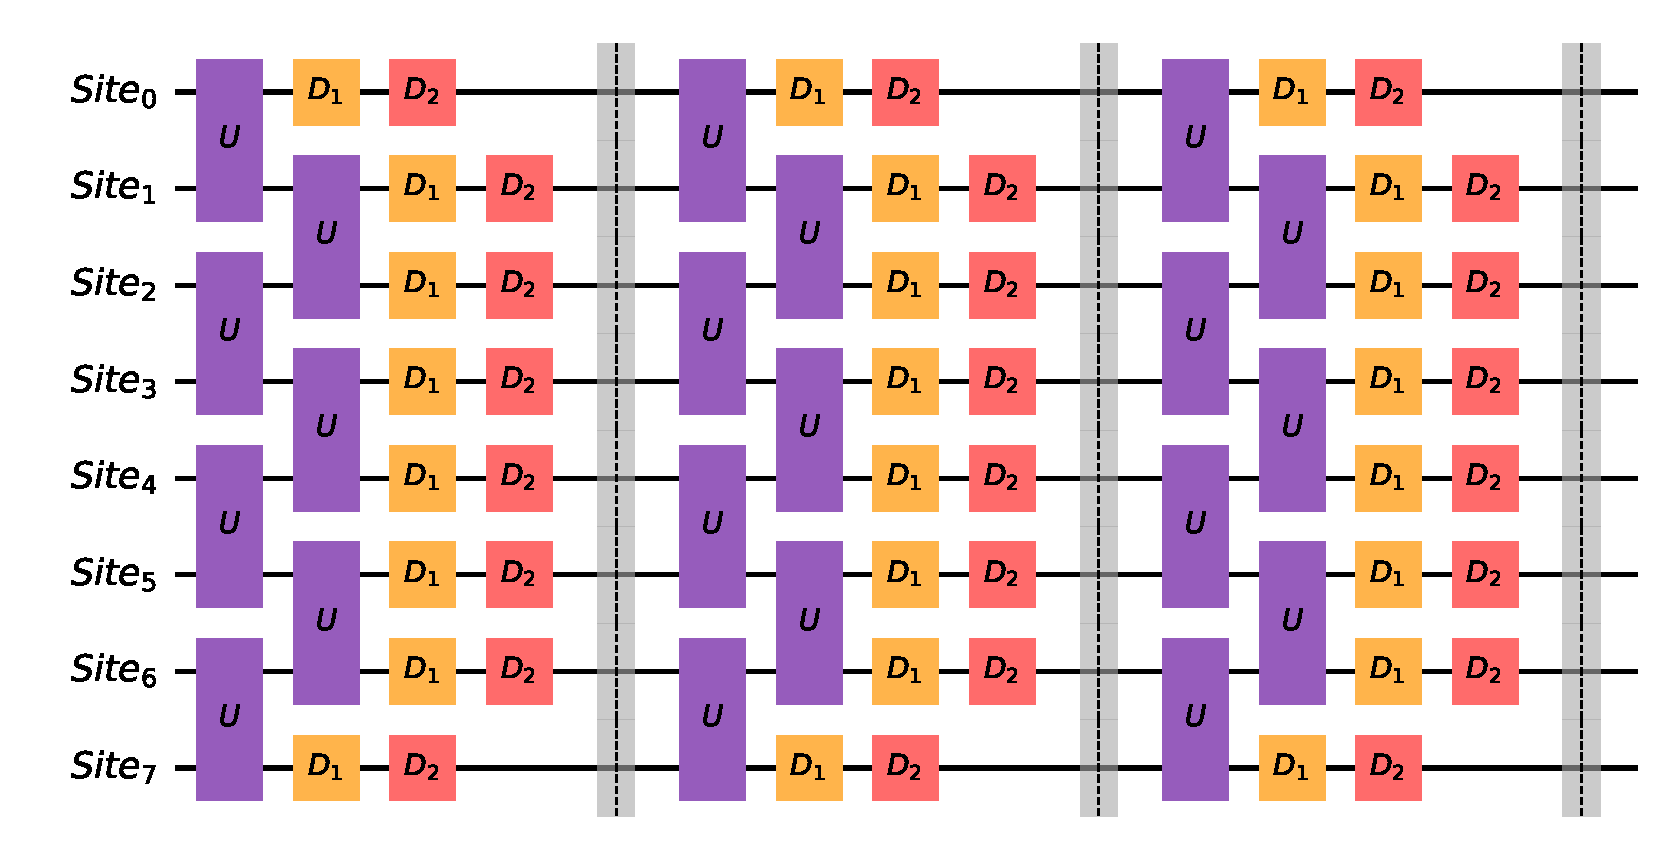
\includegraphics[width=\linewidth]{Ansatz_circuit.pdf}
    \caption{\raggedright The ansatz PQC (with 3 layers) used in this paper. Each layer consists of an alternating two-site brickwork unitaries $U$. And $D_1$ represents a single-site depolarizing noise, $D_2$ represents a single-site dephasing noise.}
    \label{fig:Ansatz_circuit}
\end{figure}

In Figure~\ref{fig:Ansatz_circuit}, we have shown the Ansatz 3-layer PQC used in this paper and future simulations. Where each ansatz PQC layer consists of an alternating two-site brickwork unitary $U$, which is constructed by taking the normalized QR decomposition of a 4-by-4 matrix, with 16 entries, and all 16 entries will be updated during the learning phase. $D_1$ represents a single-site depolarizing noise, $D_2$ represents a single-site dephasing noise. The transfer matrix corresponding to the depolarizing noise with depolarizing strength $p$ has the matrix form:

\begin{equation}
    D_1(p) = \begin{bmatrix}
        1 &0 & 0 & 0 \\
        0 & 1-4p/3 & 0 & 0\\
        0  & 0 & 1-4p/3 & 0 \\
        0  & 0 & 0 & 1-4p/3
    \end{bmatrix}
    \label{eq:Depolarizing_D_1}
\end{equation}

Where $p$ is the parameter that is modified through gradient descent in the learning phase. And the transfer matrix corresponding to the dephasing noise with dephasing strength $p$ and dephasing direction in $x, y, z$, denoted as $\mathbf{n}=(n_x, n_y, n_z)$, the matrix form can be written as

\begin{equation}
\begin{split}
    D_2(p, \mathbf{n})[\rho] &= \left(1-\frac{p}{2}\right)\rho + \frac{p}{2}\sigma \rho\sigma
\end{split}
\end{equation}

Where $\sigma = n_xX+n_yY+n_zZ$, with the normalization $n_x^2+n_y^2+n_z^2 = 1$. Thus, $D_2$ has the matrix form of:
\begin{equation}
D_2(p, \mathbf{n}) = \begin{bmatrix}
1 & 0 & 0 & 0 \\
0 & 1 - p(1 - n_x^2) & p n_x n_y & p n_x n_z \\
0 & p n_x n_y & 1 - p(1 - n_y^2) & p n_y n_z \\
0 & p n_x n_z & p n_y n_z & 1 - p(1 - n_z^2)
\end{bmatrix}
\end{equation}

In general, the Ansatz PQC can have $T$ layers, for any $T\in \mathbb{Z}^+$. \yijian{What is the expressiveness of this channel? It is definitely self-dual (i.e., no amplitude damping), but is it general enough to capture all self-dual 1 qubit channels?}
\simba{I believe we are doing a self-dual channel, no amplitude damping. I am not sure if it is general enough to cover all 1-qubit channel, I will have a look.}

\subsection{Learning and Compressing Quantum Circuit with Ansatz PQC}
We proposed that with our Ansatz circuit shown in Figure~\ref{fig:Ansatz_circuit}, a general quantum circuit with unitaries and noise can be effectively learned and compressed. And in this subsection, we briefly discuss the numerical methods used in later sections of this paper.

Most simulations and machine learning tasks are performed using Python 3.12. The handling of the Matrix Product States (MPS) and Matrix Product Operators (MPO) is done with the Quimb package. We use PyTorch as the backend for performing most of our machine learning tasks. All graphs shown are generated with the Matplotlib package. 

First, we provide a quick analysis of the number of free parameters in our Ansatz circuit that is updated during learning. A two-site transfer matrix sampled from a two-site unitary from the group $SU(4)$ has $15$ group generators, so $15$ free parameters. With an Ansatz PQC with $N$ sites, each layer contains $N-1$ two-site unitary transfer matrices. In addition, $D_1$ contains $1$ free parameter, the depolarizing strength $p$. And $D_2$ contains $4$ free parameters, $p, n_x, n_y, n_z$. Thus, each layer of our Ansatz PQC contains $15(N-1)+1+4=15N-10$ free parameters. Thus, an Ansatz PQC with $N$ sites and $T$ layers $\E_{model}^{N, T}$ contains $15NT-10T$ free parameters, which grows linearly with $N$ and $T$. While even a general $N$-site Unitary contains $N^2-1$ group generators, which scales as $N^2$.

Given a black-box quantum circuit $\E_{target}$, the learning process starts with building the Ansatz PQC $\E_{model}$ with $T$ layers. And the preparation of several training input sample Pauli strings $\{M_{in, k}\}_k$ in the MPS format. We first pass $\{M_{in}\}$ to the $\E_{target}$, and obtain the target output MPS states. $\{M_{realout}\}_k = \{\E_{target}(M_{in, k})\}_k$. 

Then, in each training epoch, we pass $\{M_{in}\}_k$ to our Ansatz PQC and obtain the output MPS in this epoch $\{M_{out}\}_k = \{\E_{model}(M_{in})\}_k$. Then, we compute the mean Frobenius distance between the set $\{M_{realout}\}_k$ and $\{M_{out}\}_k$. \yijian{Notation is a bit awkward. Should be enough to write an equation of the total loss directly}

\begin{equation}
    Loss = \frac{1}{|\{M_{in}\}_k|}\sum_k d_F\left(M_{realout, k}, M_{out, k}\right)
\end{equation}

Where $d_F$ is the Frobenius distance metric, with the loss at the current epoch, the parameters of the Ansatz PQC are updated through backwards propagation, and most of the backward propagation is done with the Adam optimizer in PyTorch.

An $N$-site Ansatz PQC $\E_{model}$ is constructed as a tensor network $TN_{model}$, with $2N$ free indices, and to get the $M_{out, k}$, we simply contract $N$ free indices of the input MPS $M_{in, k}$ and the $N$ free indices of $TN_{model}$, which left $N$ free indices in the system that represents $M_{out, k}$. Note that to make the backwards propagation process more effective, we do not compress the $TN_{model}$; we keep its tensor network form. 

When computing the Frobenius distance between $M_{out, k}$ and $M_{realout, k}$, note that the computation resources scale linearly with the number of sites in the system $N$ while exponentially in the number of layers $T$ due to finding the path for exact contraction. Thus, according to our numerical findings, running an ansatz PQC up to 3 layers can be done efficiently, and the results are promising.


\subsection{Training Dataset Generation}
\label{sec:Training_dataset_generation}

In our quantum channel learning model, we primarily use the Pauli String of weight 1 for training because we believe it provides a good learning set.

This subsection clarifies when one may replace $\mathcal{C}(AB)$ by $\mathcal{C}(A)\mathcal{C}(B)$ at the operator level.

\yijian{The following discussions are obvious.}
A (finite-dimensional) quantum channel is a completely positive,
trace-preserving (CPTP) linear map
\(\mathcal{C}:\mathcal{B}(\mathcal{H})\to\mathcal{B}(\mathcal{H})\),
where $\mathcal{B}(\mathcal{H})$ denotes the bounded operators on the system Hilbert space $\mathcal{H}$. A unitary channel is given by
\begin{equation}
  \mathcal{U}(X) = U X U^{\dagger},
  \qquad X\in\mathcal{B}(\mathcal{H}),
\end{equation}
for a unitary operator $U$ on $\mathcal{H}$. The map $\mathcal{U}$ is linear, completely positive, trace-preserving
and unital, i.e. $\mathcal{U}(\openone)=\openone$.

\begin{theorem}
Let $\mathcal{U}(X)=UXU^{\dagger}$ be a unitary channel. Then
$\mathcal{U}$ is a unital $*$-automorphism of the operator algebra
$\mathcal{B}(\mathcal{H})$: for all $A,B\in\mathcal{B}(\mathcal{H})$,
\begin{equation}
  \mathcal{U}(AB)=\mathcal{U}(A)\,\mathcal{U}(B),
  \qquad
  \mathcal{U}(A^{\dagger})=\mathcal{U}(A)^{\dagger}.
\end{equation}
In particular, if $A$ and $B$ are Pauli strings then
$\mathcal{U}(AB)=\mathcal{U}(A)\mathcal{U}(B)$.
\end{theorem}

\begin{proof}
Linearity is immediate from the definition. For the adjoint, we have
\begin{equation}
  \mathcal{U}(A^{\dagger})
  = U A^{\dagger} U^{\dagger}
  = (UAU^{\dagger})^{\dagger}
  = \mathcal{U}(A)^{\dagger}.
\end{equation}
For multiplicativity, we compute
\begin{equation}
  \mathcal{U}(AB)
  = U (AB) U^{\dagger}
  = (UAU^{\dagger})(UBU^{\dagger})
  = \mathcal{U}(A)\,\mathcal{U}(B),
\end{equation}
where we used $U^{\dagger}U=\openone$ to combine the middle factors.
Thus $\mathcal{U}$ is a $*$-homomorphism of $\mathcal{B}(\mathcal{H})$
onto itself, i.e.\ a $*$-automorphism.
\end{proof}

Therefore, whenever the channel describing the evolution is implemented by conjugation with a single unitary, products of operators (and in particular products of Pauli strings) are preserved under the channel in the sense that $\mathcal{U}(AB)=\mathcal{U}(A)\mathcal{U}(B)$.

Thus, by limiting to a single channel, all different Pauli strings can be written as products of one or more weight-1 Pauli strings. Therefore, learning how the weight-1 Pauli string changes under the unital channel suffices to capture the channel's effect on all Pauli strings.

However, a general CPTP map $\mathcal{E}$ admits a Kraus representation
\begin{equation}
  \mathcal{E}(X) = \sum_{k} K_k X K_k^{\dagger},
  \qquad \sum_{k} K_k^{\dagger}K_k = \openone.
\end{equation}
Unless there is only a single Kraus operator and it is unitary, such a map is not a $*$-homomorphism, and in general
\begin{equation}
  \mathcal{E}(AB) \neq \mathcal{E}(A)\,\mathcal{E}(B)
\end{equation}
even when $A$ and $B$ are Pauli strings.
This can be seen explicitly from
\begin{equation}
  \mathcal{E}(AB)
  = \sum_{k} K_k A B K_k^{\dagger},
  \quad
  \mathcal{E}(A)\mathcal{E}(B)
  = \sum_{k,\ell} K_k A K_k^{\dagger} K_{\ell} B K_{\ell}^{\dagger},
\end{equation}
whose cross terms with $k\neq \ell$ do not cancel in general.

But here we argue mathematically, given a target quantum circuit $\E_{target}$, in the presence of noise, the max LOE of the final MPS after the circuit $M_{out}$ corresponding to an input Pauli string MPS $M_{in}$ will be larger when the Pauli weight of the input Pauli string MPS $M_{in}$ is 1, where the Pauli weight of a Pauli string is the number of sites of the MPS that is not the identity $I$. Hence, theoretically, and later we see it numerically, that a weight-$1$ MPS will give the most prominent learning and testing loss. For demonstration purposes, we consider the depolarizing noise.

Let $N$ be the number of sites of the MPS. Denote $M_{in}= P_1\otimes\cdots P_N$, where each $P_k \in\{I, X, Y, Z\}$.
The Pauli weight of this string, denoted as $w$, is the number of sites where $P_k\ne I$. As $Tr(P^\dagger P)=2^N$. Hence, we can write the normalized input MPS as $M_i = P/\sqrt{2^N}$. Now, recall that the super-operator of depolarizing noise $D_1(p)$ has the form in Equation~\ref{eq:Depolarizing_D_1}. Hence, $D_1(p)[I]=I$, while $D_1(p)[P_k]=(1-4p/3)P_k$ for $P_k\in\{X, Y, Z\}$. Hence, in our Ansatz circuit, when we add a layer of depolarizing noise,
\begin{equation}
\begin{split}
    M' &= \frac{1}{\sqrt{2^N}}\left(\E(P_1)\otimes \cdots\otimes \E(P_N)\right)\\
    &=\frac{1}{\sqrt{2^N}}\left((1-4p/3)^w P\right)
\end{split}
\end{equation}

%Can add in K-local MPS

Hence, the Frobenius norm of the MPS $M$ is suppressed by a factor of $(1-4p/3)^w$ per layer of depolarizing operator with strength $p$. Hence, the higher the initial Pauli weight of the MPS $M$, the smaller the $\norm{M_{out}}_F$. Thus, to generate a useful training set, we use the first non-trivial set of the Pauli strings, which is the set of all weight-1 Pauli strings. \yijian{The argument does not seem to be very solid, so a numerical justification should be needed - i.e., training with weight-1 and weight-2 operators does not give different results; or, training with weight-1 could be used to test on weight 2.}
\simba{I have added a section of numerical justification in future sections.}

Later in Section \simba{XXXX}, we have shown numerical evidence that using only the complete structured set of weight-1 Pauli strings, the model's training and testing loss is lower than using an order of magnitude more random Pauli string inputs.

\subsection{Weight-1 sufficiency in the intermediate-noise regime}
\label{sec:intermediate_noise_sufficiency}

\simba{The arguments in this subsections are are more sketchy, so we can put this subsection in the appendix instead.}
The arguments above cover two limiting regimes: (i) the unitary limit ($p\to 0$), where $\mathcal{U}(AB) = \mathcal{U}(A)\mathcal{U}(B)$ makes weight-1 Paulis a generating set under multiplication, and (ii) the high-noise limit, where the Frobenius-norm suppression $(1-4p/3)^{wL}$ concentrates the loss on low Pauli weights. Neither argument is rigorous at \emph{intermediate} noise strengths $p\sim 0.02$--$0.1$, where most of the paper's numerical experiments lie. In this subsection we give a structural argument, tailored to our specific PQC family (layers of 2-site unitaries composed with single-site Pauli channels), that fills this gap.

\paragraph*{Key structural property: disjoint-support multiplicativity.}
The non-$*$-homomorphism property of a general CPTP map (Eq.~\eqref{eq:Depolarizing_D_1} and the theorem above) fails \emph{generally}, but a weaker multiplicativity property holds for our PQC's single-layer structure. The building block of this property is that single-site Pauli channels act \emph{diagonally} in the Pauli basis, with real eigenvalues that are directly observable from randomized-benchmarking-type experiments~\cite{magesan2012characterizing,flammia2020pauli,harper2020efficient}. We formalize this below in the form used throughout this paper.

%\todoflag{\emph{Provenance of the statement.} Theorem~\ref{thm:disjoint_multiplicativity} is our own packaging of standard ingredients, tailored to the PQC-identifiability question of this subsection. None of the individual ingredients is new: (i) the Pauli-diagonal structure of single-site Pauli channels (used in the proof) is textbook material~\cite[\S8.3]{nielsen2010quantum}\cite{watrous2018theory,nielsen2002simple,magesan2012characterizing}; (ii) the tensor-product factorization of $\mathcal{N}_\ell = \bigotimes_k \mathcal{N}_{\ell,k}$ across disjoint sites is exploited explicitly in the Pauli-channel-learning literature~\cite{flammia2020pauli,harper2020efficient} and underlies the noise-tailoring-by-randomized-compiling protocol of Wallman and Emerson~\cite{wallman2016noise}; (iii) the unitary $*$-homomorphism is the content of the theorem at the start of this subsection and is standard~\cite{nielsen2010quantum,watrous2018theory}. The same factorization property is implicit in the Pauli-frame / stabilizer simulation of noisy Clifford circuits~\cite{aaronson2004stabilizer} and in the Pauli-error-model analyses of fault-tolerant protocols~\cite{knill2005quantum}. What is (to our knowledge) not stated in the literature as an explicit named theorem is the combination of these three facts for PQC layers of the specific form $\mathcal{N}\circ\mathcal{U}$ with local $\mathcal{U}$, which we therefore record as Theorem~\ref{thm:disjoint_multiplicativity} for use in the identifiability argument of Corollary~\ref{cor:single_layer_identifiability}.}

\begin{theorem}[Single-layer disjoint-support multiplicativity]
\label{thm:disjoint_multiplicativity}
Let $\mathcal{C}_\ell := \mathcal{N}_\ell\circ\mathcal{U}_\ell$ be \emph{one} layer of our PQC family, where $\mathcal{U}_\ell$ is a unitary channel (in our setting, a product of nearest-neighbour two-site unitaries) and $\mathcal{N}_\ell = \bigotimes_{k=1}^N\mathcal{N}_{\ell,k}$ is a tensor product of single-site Pauli channels. For any two Pauli strings $P,Q$ such that the operator supports of $\mathcal{U}_\ell(P)$ and $\mathcal{U}_\ell(Q)$ remain disjoint after the layer unitary --- equivalently, the one-layer light cones of $\mathrm{supp}(P)$ and $\mathrm{supp}(Q)$ do not meet --- one has
\begin{equation}
    \mathcal{C}_\ell(PQ) \;=\; \mathcal{C}_\ell(P)\,\mathcal{C}_\ell(Q).
    \label{eq:disjoint_mult}
\end{equation}
For a brickwork unitary in which every pair of neighbouring sites is acted on by a two-qubit brick in the layer, the light-cone condition reduces to $\mathrm{dist}\bigl(\mathrm{supp}(P),\mathrm{supp}(Q)\bigr)\ge 3$.
\end{theorem}

\begin{proof}
Write $\mathcal{N}_{\ell,k}(X) = \lambda_k(X)\,X$ for $X\in\{I,\sigma_x,\sigma_y,\sigma_z\}$ (each $\mathcal{N}_{\ell,k}$ is Pauli-diagonal, so it acts as a multiplier on single-site Paulis; see Refs.~\cite{nielsen2002simple,magesan2012characterizing,flammia2020pauli}). By the $*$-homomorphism property of unitary channels~\cite{nielsen2010quantum,watrous2018theory}, $\mathcal{U}_\ell(PQ)=\mathcal{U}_\ell(P)\mathcal{U}_\ell(Q)$, and the operands $\mathcal{U}_\ell(P),\mathcal{U}_\ell(Q)$ have disjoint supports by hypothesis. For two Pauli strings $A,B$ with disjoint supports, $\mathcal{N}_\ell(AB) = \lambda(A)\lambda(B)\,AB = \bigl[\lambda(A)A\bigr]\bigl[\lambda(B)B\bigr] = \mathcal{N}_\ell(A)\,\mathcal{N}_\ell(B)$ because single-site Paulis on disjoint sites commute and their $\lambda$-factors multiply site-by-site. Applying this to $A=\mathcal{U}_\ell(P)$, $B=\mathcal{U}_\ell(Q)$ gives $\mathcal{N}_\ell(\mathcal{U}_\ell(PQ))=\mathcal{N}_\ell(\mathcal{U}_\ell(P))\mathcal{N}_\ell(\mathcal{U}_\ell(Q))$, i.e.\ Eq.~\eqref{eq:disjoint_mult}.
\end{proof}

Note that, this theorem is a \emph{single-layer} statement and does not extend verbatim to multi-layer PQCs. For $T$ layers, iterating the argument requires $\mathcal{U}_T\circ\cdots\circ\mathcal{U}_1(P)$ and $\mathcal{U}_T\circ\cdots\circ\mathcal{U}_1(Q)$ to retain disjoint supports, which holds if and only if the lattice-distance between $\mathrm{supp}(P)$ and $\mathrm{supp}(Q)$ exceeds $2T$. For the typical experimental parameters of this paper ($N=8$, $T=3$), only the pair of extreme-end sites $(1,8)$ satisfies this, so the direct multi-layer generalization applies to almost no weight-1 pairs. Consequently Theorem~\ref{thm:disjoint_multiplicativity} \emph{by itself} does not establish multi-layer identifiability from weight-1 inputs. It plays the role of a structural single-layer fact that, together with the over-determination, operator-spreading, underpins the multi-layer argument.

%\paragraph*{Single-layer identifiability from weight-1 inputs.}
As an immediate corollary, one layer of the PQC family is uniquely determined by its action on weight-1 Paulis. \yz{doesn't this mean for 1d, k layers you need weight $2k-1$?}

\begin{corollary}[Single-layer identifiability]
\label{cor:single_layer_identifiability}
Let the layer superoperator act on an input Pauli $P$ as $\mathcal{C}_\ell(P):= \mathcal{U}_\ell(\mathcal{N}_\ell(P))$, i.e.\ the operator is first acted on by the tensor-product single-site Pauli noise $\mathcal{N}_\ell$ and then by the unitary $\mathcal{U}_\ell(\cdot) = U_\ell(\cdot)U_\ell^{\dagger}$. (This is the operator-flow order used for PTM propagation in this paper; see the circuit of Fig.~\ref{fig:Ansatz_circuit} read in the Heisenberg-like operator direction.) Suppose $\mathcal{C}_\ell^{(a)}$ and $\mathcal{C}_\ell^{(b)}$ are two such layers with identical two-site brickwork support pattern, and that
\begin{equation}
    \begin{split}
        \mathcal{C}_\ell^{(a)}(P_k) \;&=\; \mathcal{C}_\ell^{(b)}(P_k)\\
        &\text{for every site }k\text{ and every }P_k\in\{X,Y,Z\}.
    \end{split}
\end{equation}
Then the single-site noise parameters of $\mathcal{N}_\ell^{(a)}$ and $\mathcal{N}_\ell^{(b)}$ agree, and $U_\ell^{(a)} = e^{i\phi}\,U_\ell^{(b)}$ for some global phase $\phi\in\mathbb{R}$. Consequently $\mathcal{C}_\ell^{(a)}=\mathcal{C}_\ell^{(b)}$ as channels.
\end{corollary}

\begin{proof}
The proof does \emph{not} invoke Theorem~\ref{thm:disjoint_multiplicativity}: it only uses (i) that single-site Pauli channels act diagonally on single-site Paulis with \emph{real} eigenvalues $\lambda_k(P)\in[-1,1]$~\cite{nielsen2002simple,magesan2012characterizing,flammia2020pauli,harper2020efficient}, and (ii) a standard commutant fact for weight-1 Paulis in $M_{2^N}$.

\emph{Step 1: extract the noise multipliers.} For a weight-1 input $P_k$, tensor-product factorization of $\mathcal{N}_\ell$ across sites gives $\mathcal{N}_\ell(P_k) = \lambda_k(P_k)\,P_k$ (all factors $\mathcal{N}_{\ell,j}(I)=I$ for $j\ne k$; site $k$ contributes the real scalar $\lambda_k(P_k)$). The unitary layer then conjugates this single Pauli, producing
\begin{equation}
    \mathcal{C}_\ell(P_k) \;=\; \lambda_k(P_k)\,U_\ell\,P_k\,U_\ell^{\dagger}.
    \label{eq:Cl_clean}
\end{equation}
This is the structural observation underlying Pauli-channel learning protocols~\cite{flammia2020pauli,harper2020efficient}. The Frobenius norm gives $\norm{\mathcal{C}_\ell(P_k)}_F = |\lambda_k(P_k)|\sqrt{2^N}$, fixing $|\lambda_k(P_k)|$; because $\lambda_k(P_k)$ is real, comparing the two channels on the \emph{operator} level (rather than only on norms) disambiguates the sign. Thus $\lambda_k^{(a)}(P_k)=\lambda_k^{(b)}(P_k)$ for every site $k$ and Pauli $P_k\in\{X,Y,Z\}$, recovering all single-site noise parameters of both layers.

\emph{Step 2: extract the unitary action.} Dividing Eq.~\eqref{eq:Cl_clean} by the common scalar $\lambda_k(P_k)$ (the corner case $\lambda_k(P_k)=0$, corresponding to a fully depolarizing channel at site $k$, makes $\mathcal{N}_\ell(P_k)$ a tensor product with a zero factor at site $k$ and hence the zero operator, so $\mathcal{C}_\ell(P_k)=0$ on this particular probe and the input carries no information about $U_\ell$; such sites must therefore be excluded from the reconstruction),
\begin{equation}
    U_\ell^{(a)}\,P_k\,(U_\ell^{(a)})^{\dagger} \;=\; U_\ell^{(b)}\,P_k\,(U_\ell^{(b)})^{\dagger} \qquad \forall k,\; \forall P_k\in\{X,Y,Z\}.
    \label{eq:conjugate_equal}
\end{equation}

\emph{Step 3: commutant argument on the full-layer unitary.} Let $W := (U_\ell^{(a)})^{\dagger} U_\ell^{(b)} \in U(2^N)$. Eq.~\eqref{eq:conjugate_equal} rewrites as $W\,P_k\,W^{\dagger} = P_k$ for all weight-1 Paulis $P_k$, i.e.\ $W$ commutes with every weight-1 Pauli. The set $\{X_k,Y_k,Z_k\}_{k=1}^{N}$ spans $\bigoplus_{k=1}^{N}\mathfrak{su}(2)_k$; taking linear combinations and including the identity spans, site-by-site, the full matrix algebra at each site. By iterative application of the elementary fact that the commutant of $I^{\otimes (k-1)}\otimes M_2 \otimes I^{\otimes(N-k)}$ in $M_{2^N}$ equals $M_{2^{k-1}}\otimes I \otimes M_{2^{N-k}}$, the joint commutant of all single-site Pauli algebras is $\mathbb{C}\cdot I_{2^N}$. Hence $W = e^{i\phi}\,I_{2^N}$ for some $\phi\in\mathbb{R}$, i.e.\ $U_\ell^{(a)} = e^{-i\phi}\,U_\ell^{(b)}$. This phase is immaterial for the channel, so $\mathcal{U}_\ell^{(a)}=\mathcal{U}_\ell^{(b)}$ and therefore $\mathcal{C}_\ell^{(a)}=\mathcal{C}_\ell^{(b)}$.
\end{proof}

Note that this corollary relies on real-valued Pauli-channel eigenvalues, which hold for depolarizing and dephasing (as defined in Sec.~\ref{sec:PQC_topology}) but not for general non-unital CPTP maps. Under these assumptions the corollary is tight, but its extension to multi-layer PQCs is not automatic and rests on the three complementary arguments (A)--(C) of the next paragraphs.

\paragraph*{Extension to multi-layer PQCs.}
Corollary~\ref{cor:single_layer_identifiability} assumes access to the input-output behaviour of a \emph{single} layer. In practice, only the cumulative $\E = \mathcal{C}_T\circ\cdots\circ\mathcal{C}_1$ is observed. Three complementary arguments establish that weight-1 training of the full multi-layer PQC is still (generically) sufficient to identify all parameters at intermediate noise.

\emph{(A) Over-determination by parameter count.}
The PQC family has $(15(N-1)+5N)\,T = (20N-15)T$ real parameters per layer~\cite{khatri2019qaqc,benedetti2019pqc}. A weight-1 Pauli input produces an output supported within the forward light cone of width $2T+1$ (by the operator-spreading bound of Refs.~\cite{nahum2018operator,vonKeyserlingk2018operatorhydrodynamics,chen2018operator}), so the non-trivial output Pauli components per weight-1 input number at most $4^{2T+1}$. With $3N$ independent weight-1 inputs, the total number of measurable linear constraints is $\mathcal{O}(3N\cdot 4^{2T+1})$. For $N=8$, $T=3$ this is $\sim 4\times 10^5$, vastly exceeding the $\sim 4\times 10^2$ parameters. The ratio of constraints to parameters places weight-1 training well within the sample-efficient regime analysed for Pauli-based tomographic protocols~\cite{flammia2011direct,huang2020predicting,mohseni2008tomography}. The parameter-to-output map $\alpha\mapsto\{\E_\alpha(P)\}_{w(P)=1}$ is a real-analytic (in fact polynomial) map between real algebraic varieties. By the generic-rank theorem for such maps~\cite{Sontag1998,bochnak1998realalgebraic}, the locus where the Jacobian fails to attain its maximum rank is the common zero set of the maximal minors and is therefore a proper Zariski-closed (hence measure-zero) subvariety of parameter space. Together with the existence of a single $\alpha$ at which the Jacobian has full column rank---realized by any non-degenerate entangling brickwork, since the $2T+1$-site light cone exposes every gate parameter to the weight-1 outputs---this implies that the Jacobian has full column rank on a Zariski-open dense subset, making weight-1 training a \emph{locally} well-posed identification problem outside a measure-zero set of pathological configurations. We emphasize that ``locally'' is needed: continuous gauge equivalences (the global phase of each $U_\ell$ in Corollary~\ref{cor:single_layer_identifiability}, and adjacent-layer redefinitions of the form $U_{\ell+1}\,V^{\dagger}\cdot V\,U_\ell$) preclude global injectivity even on the full-rank locus, and weight-1 training identifies $\E_\alpha$ only up to these gauge symmetries.

\emph{(B) Operator spreading covers the full Pauli basis probed by later layers.}
Under layer $\mathcal{C}_1$, a weight-1 input spreads to a linear combination of Paulis of weights in $\{1,2,3\}$ supported on three adjacent sites (the one-layer light cone)~\cite{nahum2018operator,vonKeyserlingk2018operatorhydrodynamics}. Inductively, after $\ell$ layers, a weight-1 input is represented as a linear combination of Paulis of weight up to $2\ell+1$. The layer $\mathcal{C}_{\ell+1}$ therefore \emph{receives} inputs that span the full relevant Pauli subspace within the light cone, not only weight-1. Since each layer in isolation is identifiable from weight-1 inputs by Corollary~\ref{cor:single_layer_identifiability}, and since weight-1 training of the full PQC exposes each layer to a representative set of higher-weight inputs via the spreading of the previous layers, the composite parameter identification is (generically) well-posed. A fully rigorous proof would require tracking the Jacobian rank through the composition in the spirit of gate-set tomography~\cite{greenbaum2015gst}; we leave this to future work but note that our numerical experiments (Sec.~\ref{sec:Numerical_result_Random_U}--\ref{sec:Numerical_result_Lindbladian}) never encountered rank degeneracy.

\emph{(C) Quantitative loss dominance.}
Decompose the total PTM-Frobenius loss by input Pauli weight, $F = \sum_{w=1}^N F_w$, where
\begin{equation}
    F_w \;:=\; \frac{1}{d^2}\sum_{\nu:\,w(\nu)=w} \bigl\|\E(P_\nu)-\E^{QMLM}(P_\nu)\bigr\|_F^2.
\end{equation}
Using the triangle inequality on Frobenius norms and the single-site depolarizing bound $\norm{\mathcal{N}_\ell(P_\nu)}_F \le (1-4p/3)^{w(\nu)}\norm{P_\nu}_F$ iterated through $L$ target layers and $T$ model layers~\cite{nielsen2002simple,magesan2012characterizing}, we obtain the layer-by-layer norm estimate
\begin{equation}
    \begin{split}
    F_w \;&\le\; \binom{N}{w}\,3^w\,\Bigl(q^{wL}+(q')^{wT}\Bigr)^2, \\
    \qquad q &:= 1-\tfrac{4p}{3},\;\; q' := 1-\tfrac{4p'}{3}.
    \end{split}
    \label{eq:F_w_bound}
\end{equation}
Under the norm-matching prescription of Sec.~\ref{sec:peak_prediction} ($q^L = (q')^T$), Eq.~\eqref{eq:F_w_bound} simplifies to $F_w \le 4\binom{N}{w}3^w q^{2wL}$. Writing $x := q^{2L}$, the ratio of higher-weight to weight-1 contributions is bounded by
\begin{equation}
    \frac{F_w}{F_1} \;\le\; \frac{\binom{N}{w}\,3^{w-1}\,x^{w}}{N\,x} \;=\; \binom{N}{w}\,\frac{3^{w-1}}{N}\,x^{w-1},
    \label{eq:Fw_over_F1}
\end{equation}
which for any fixed $w\ge 2$ is exponentially small in $L$ once $x\ll 1$. Consequently, whenever the cumulative target noise is non-trivial ($q^{L}$ not close to $1$), the high-weight contributions to the loss are suppressed relative to the weight-1 contribution by the factor in Eq.~\eqref{eq:Fw_over_F1}. Minimizing $F_1$ to precision $\epsilon$ therefore bounds the total loss $F$ within a $p$-dependent constant times $\epsilon$. Specifically for our Sec.~\ref{sec:Numerical_result_Random_U} regime $p\in[0.02,0.1]$, $L\in[3,25]$, Eq.~\eqref{eq:Fw_over_F1} gives $F_w/F_1\lesssim 1$ uniformly for $w\ge 2$, so weight-1 training captures the dominant contribution to the full loss.

\subsection{Numerical Justification of using Weight-1 Pauli Strings}

\begin{figure*}
    \centering
    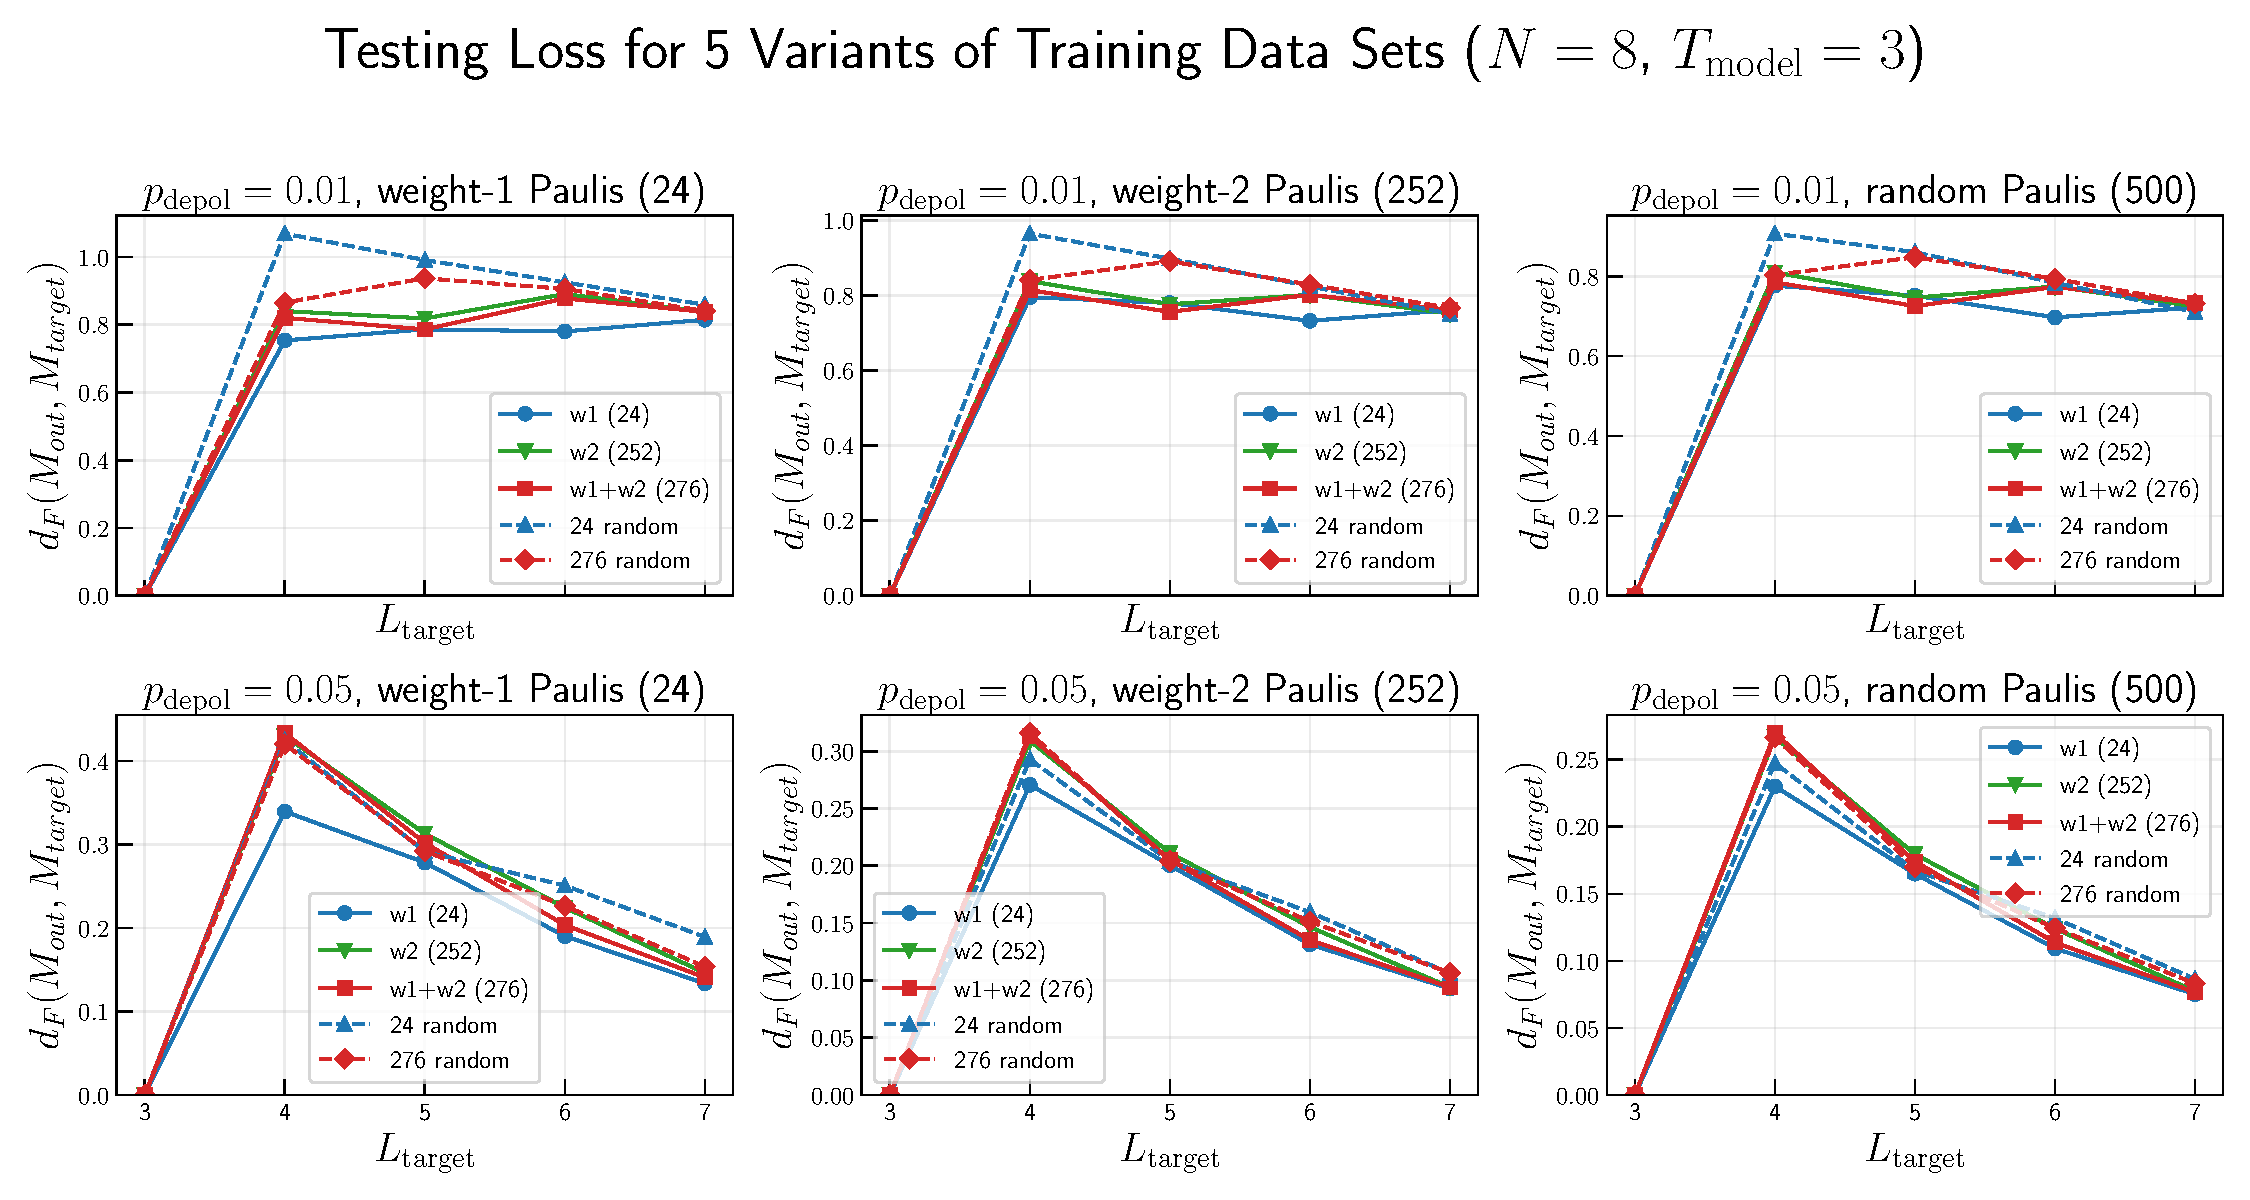
\includegraphics[width=0.8\textwidth]{five_variant_extended.pdf}
    \caption{\raggedright Mean Frobenius distance $d_F(M_{\rm out}, M_{\rm target})$ between model PQC and target PQC outputs versus the target PQC depth $L_{\rm target}$ for five training-set choices ($N=8$ qubits, $T_{\rm model}=3$, $240$ epochs): the set of full weight-1 Pauli strings(\textit{w1, 24}), full weight-2 Pauli strings (\textit{w2, 252}), their union (\textit{w1+w2, 276}), and the randomly sampled Pauli strings baselines of matched size (\textit{24/276 random}), evaluated on three held-out sets (arranged in columns: complete weight-1 basis, complete weight-2 basis, $500$ random Paulis inputs) at two depolarizing strengths (arranged in rows: $p_{\rm depol}\in\{0.01, 0.05\}$).}
    \label{fig:five_variant_compare}
\end{figure*}

%Firstly, a clear observation on the dynamics of PQC is that, long-range entanglements are exponentially suppressed, as the affective region of each qubit site grows with the light-cone, which suffers from noise layer after passing through each layer. Thus, as discussed above, we are mostly interested in only low-weight pauli behaviour, and use them as the training dataset.

To assess how strongly the choice of training inputs steers the trained channel, we compare five different training sets at matched architecture ($N=8$ qubits, $T_{\rm model}=3$ model PQC layers, target PQC of depth $L_{\rm target}\in\{3,4,5,6,7\}$ with per-layer depolarizing noise $p_{\rm depol}\in\{0.01,0.05\}$) as we have discussed in the PQC structure: %the complete weight-$1$ Pauli basis (\textit{w1}, $24$ inputs), the complete weight-$2$ Pauli basis (\textit{w2}, $252$ inputs), their union (\textit{w1+w2}, $276$ inputs), and two random-Pauli baselines of the same cardinalities (\textit{24 random}, \textit{276 random}), each drawn uniformly over Pauli strings with weight $w\sim\mathrm{Unif}[1,N]$ and uniformly distributed support and operator labels.

\begin{enumerate}
    \item Full weight-1 Pauli strings: 24 samples in total.
    \item Full weight-2 Pauli strings: 252 samples in total.
    \item Full weight-1 plus full weight-2 Pauli strings: 276 samples in total.
    \item 24 randomly sampled Pauli strings.
    \item 276 randomly sampled Pauli strings.
\end{enumerate}

The randomly sampled Pauli strings are individually drawn uniformly over Pauli strings with weight $w\sim\mathrm{Unif}[1,N]$ and uniformly distributed support and operator labels.

The main findings, as shown in Figure~\ref{fig:five_variant_compare}, is that the smallest structured training set, i.e., the $24$ weight-$1$ inputs, yields the smallest mean Frobenius distance $d_F(M_{\rm out},M_{\rm target})$ across every evaluation set we considered and at almost every depth $L_{\rm target}\geq 4$, where the target lies outside the model family, despite using more than an order of magnitude fewer training samples than the next-largest set.

%$: weight-$1$ training beats weight-$2$ training by $\sim\!10$--$30\%$ and beats combined training by $\sim\!5$--$15\%$ on the random-Pauli evaluation set at $p_{\rm depol}=0.05$, even though the combined training loss is dominated ($\sim\!91\%$) by the $252$ weight-$2$ inputs by virtue of the unweighted mean over the $276$-input loss.

Comparing the structured set to a uniformly-random Pauli set of the same cardinality isolates the contribution of the input geometry from raw sample count: at $24$ inputs the structured weight-$1$ basis is better than the $24$ random inputs across the saturated regime $L_{\rm target}\geq 4$, while at $276$ inputs the structured combined basis is also better than $276$ random inputs.

%We attribute this asymmetry to the natural alignment between the QMLM parameterization --- $T$ layers of per-pair two-site unitaries composed with per-site single-qubit noise channels --- and the weight-$1$ Pauli basis: a weight-$1$ input $P=\sigma_\alpha^{(i)}$ has identity at every site $j\neq i$, so the gradient of the loss with respect to each per-site noise channel and each two-site gate is sparse, with non-zero contributions only from primitives along the input's light-cone; the resulting Jacobian is near-diagonal in parameter space and gives an essentially independent estimator for each per-site noise rate, much like single-qubit-Pauli process tomography for tensor-product noise models~\cite{flammia2020pauli}. Weight-$2$ and higher-weight inputs, by contrast, couple multiple per-site primitives in each gradient contribution, producing a dense Jacobian whose least-squares projection onto the model family selects a channel that is biased away from the operationally relevant per-site directions; the optimiser therefore lands in a basin that fits the training subspace but generalises less cleanly to operators of other weights.

Thus, we have shown numerical evidence that, for the noise-channel-plus-brickwall PQC architecture studied in this paper, the optimal and most efficient training-set choice is the cheapest one: $3N$ weight-$1$ Pauli inputs both minimise sample-generation cost and provide the optimal training results as demonstrated in the examples shown above. This echos with our theoretical estimation in the previous section \simba{which section}, that using the complete structured set of weight-1 Pauli strings as the input is sufficient in training the PQC.


%In this sub-section, we demonstrate numerical evidence of why using the set of weight-1 pauli strings as the training dataset is mostly sufficient. As a comparison, we run a training model with $N=8$ qubit sites, the model PQC $\E_{model}$ with layer $T=3$, and the target PQC $\E_{target}$ with layer $L_{target}=\{3, 4, 5, 6, 7\}$. And we trained the $\E_{model}$ for 200 training epoches using the following five different training datasets:




\section{Compressing Harr Random Unitaries with Noise}
\label{sec:Numerical_result_Random_U}

We will briefly discuss the procedure for compressing a Haar-random channel with noise. 

Firstly, we fix the number of qubits $N$ used in our simulation, then the number of layers in our model PQC $T_{PQC}$, which is the PQC that we will modify the parameters through backwards propagation in each learning epoch. To initialize, all two-site unitaries are set to be the identity in the operator basis at first, and all noise, both depolarizing and dephasing, is set to 0; we shall call this channel $\E_{PQC}$. Note that $\E_{PQC}$ is in the form of an MPO, which is not compressed.

Then, we will randomly generate a channel to be learned, which has the same structure as a PQC with $L_{target}$ layers, and in each layer, the 2-site unitaries are initialized to be Haar-random unitaries, where the one-site noise, both depolarizing and dephasing, are assigned to different values depending on different settings, which we will show later in results, we shall call this channel $\E_{target}$.

The primary research question is whether, in the presence of noise with various strengths, we can compress a target PQC with $L_{target}$ layers with another shorter model PQC with $T_{PQC}$ layers, such that for randomly sampled Pauli String input, the output states are similar enough.

It is widely known that in the unitary limit, where the noise is zero, the complexity of the PQC grows linearly with the number of layers until it saturates. Thus, it is impossible to compress a long PQC without noise. However, in another extreme, for sufficiently large depolarizing noise, the channel will be effectively a total depolarizing channel, which can be simulated effectively using a 1-layer PQC with high enough noise.

Therefore, we would like to see the intermediate case, for some finite but non-zero noise happening at each gate, whether it is possible to compress the PQC? We believe yes, and our machine learning results have shown moderate success. 

We first generate the training dataset, where the inputs are all $3N$ weight-$1$ Pauli strings $\{P^1_{i}\}_{i=1}^{3N}$ as MPS without entanglements, and the output is obtained by propagating each $P^1_i$ through $\E_{target}$ and obtaining a set of MPS $\{M_{target, i}\}_{i=1}^{3N}$, if necessary, we perform truncation to the MPS bond dimension to ensure the learning efficiency without losing much of the information.


In each training epoch, we propagate through all weight-$1$ Pauli strings $\{P^1_{i}\}_{i=1}^{3N}$ with (uncompressed) $\E_{PQC}$, gaining a big tensor network $M_{out, i}$, and we compute the individual loss using the Frobenius distance $d_F(M_{target, i}, M_{out, i})$, which is well-defined as they have the same outer indices. The mean of all individual losses calculates the training loss of each epoch.

\begin{equation}
    \text{training loss}=\frac{\sum_{i=1}^{3N}d_F(M_{target, i}, M_{out, i})}{3N}
\end{equation}


One of the key advantages of our machine learning code is the low computational resources needed. All the presented simulation results were generated within a reasonable time frame (a few hours) using a 2022 MacBook Pro. 

\subsection{Exact Channel Learning for 8 Sites}

\begin{figure}
\centering
\begin{subfigure}{\linewidth}
    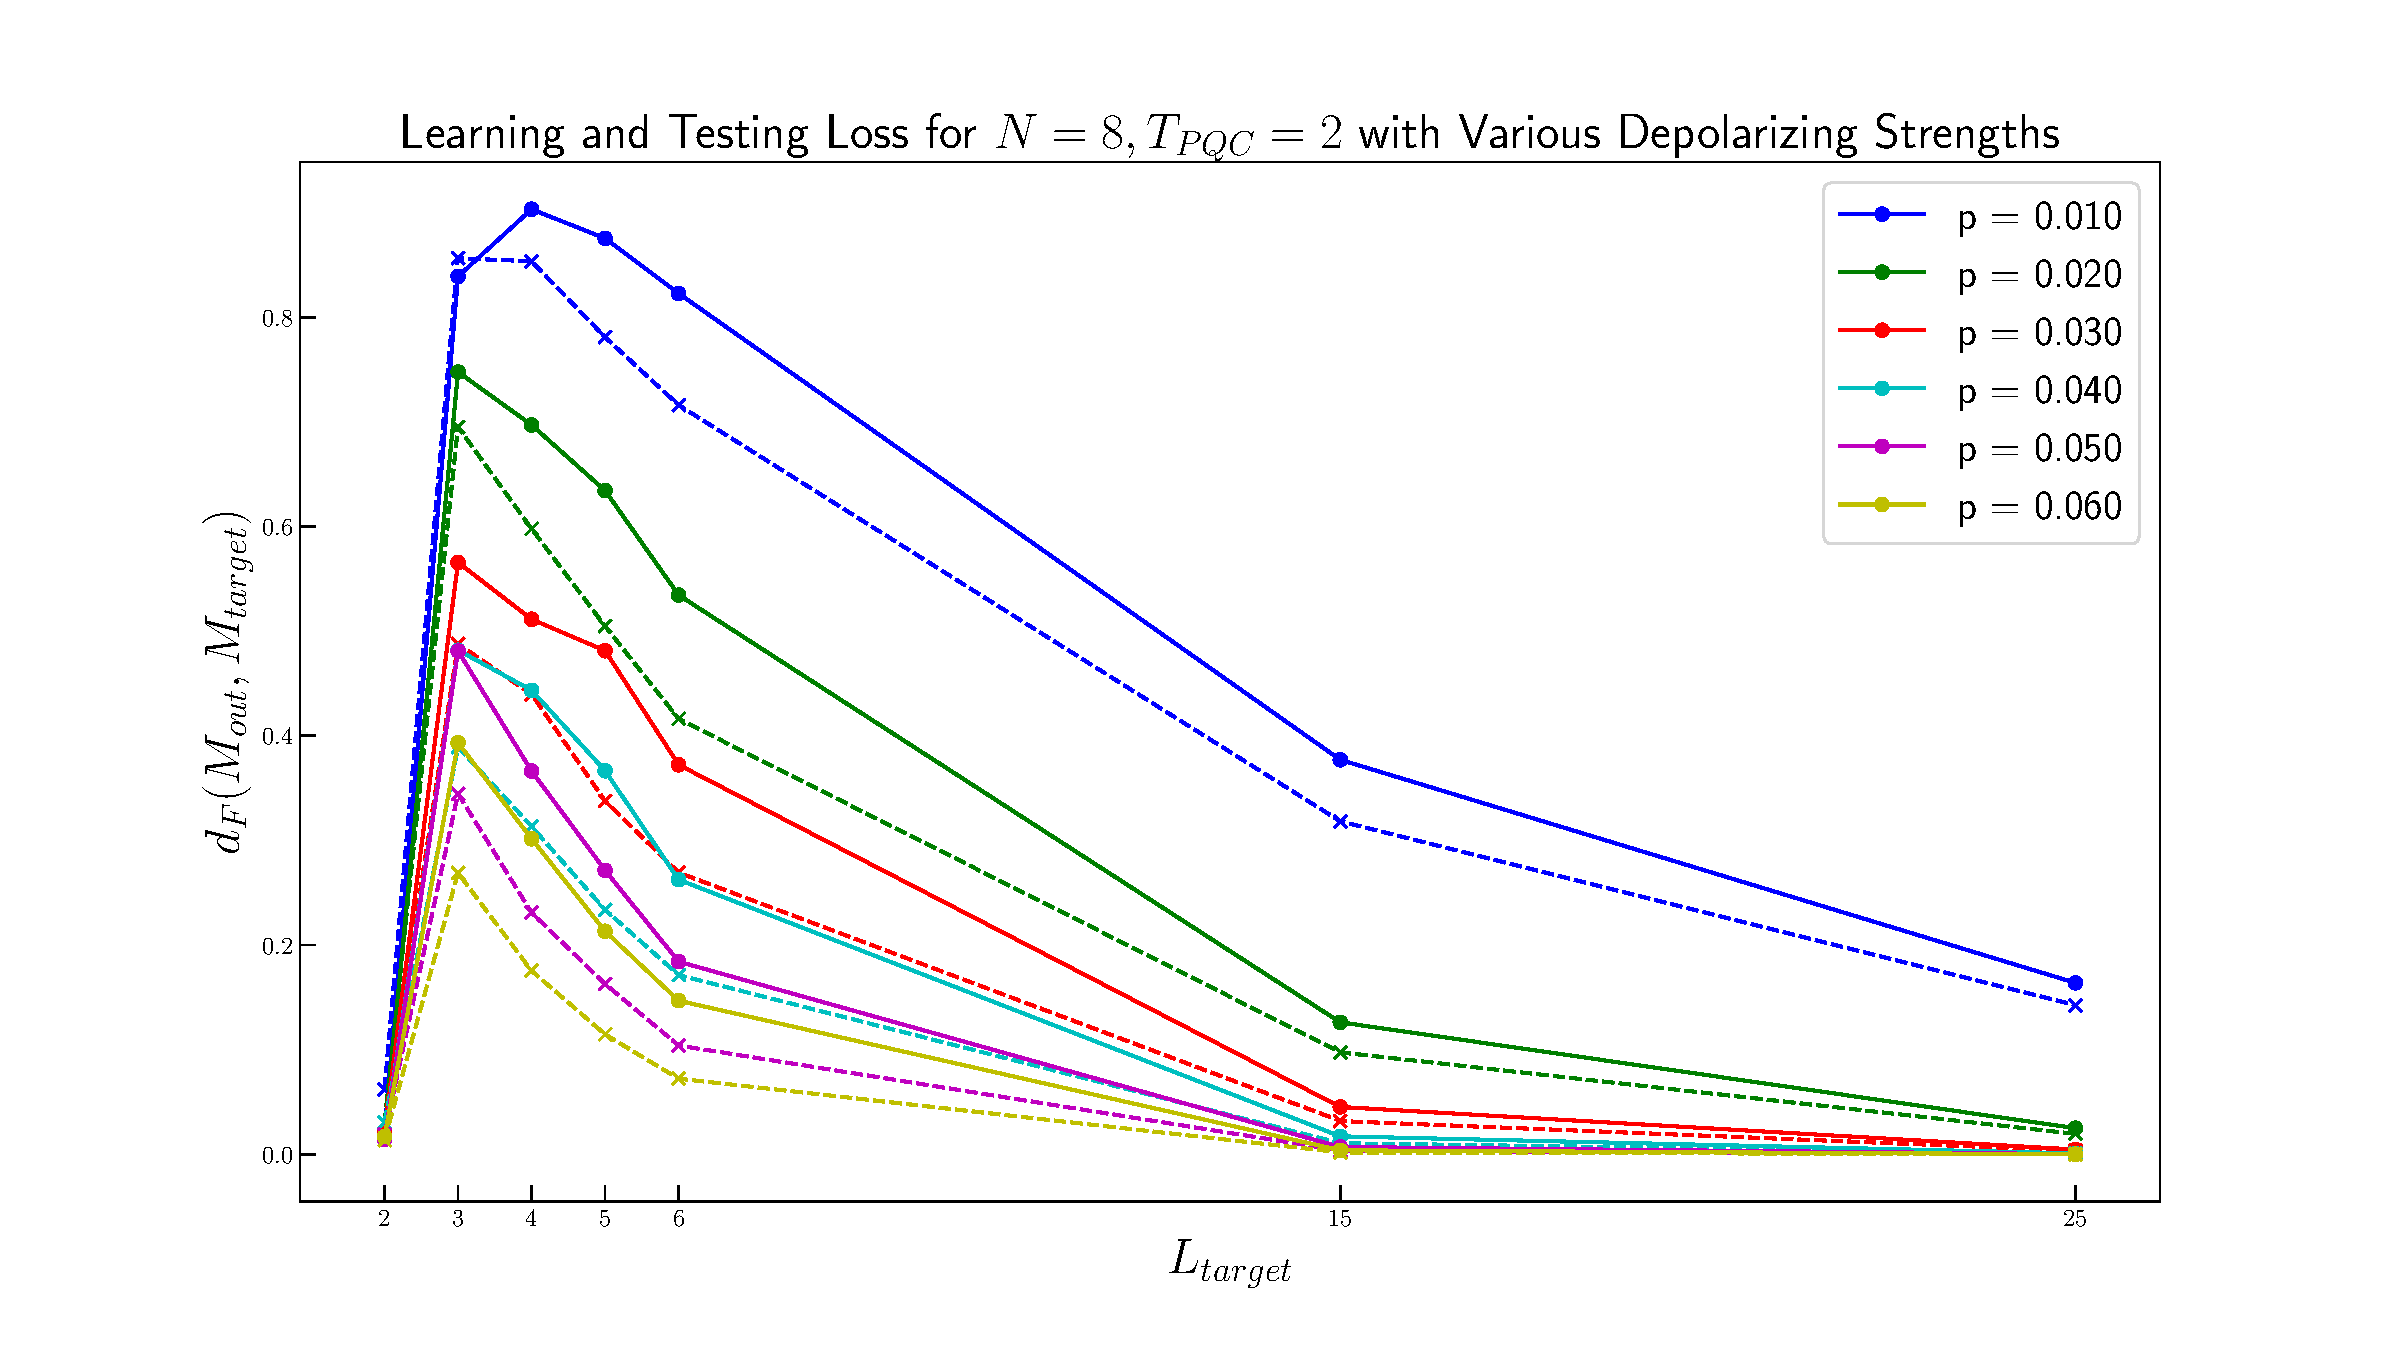
\includegraphics[width=\linewidth]{Depolarizing_ChangeT_N_L_p_8_2_all.pdf}
    \caption{}
    \label{fig:Depolarizing_ChangeT_N_L_p_8_2_all}
\end{subfigure}
\hfill
\begin{subfigure}{\linewidth}
    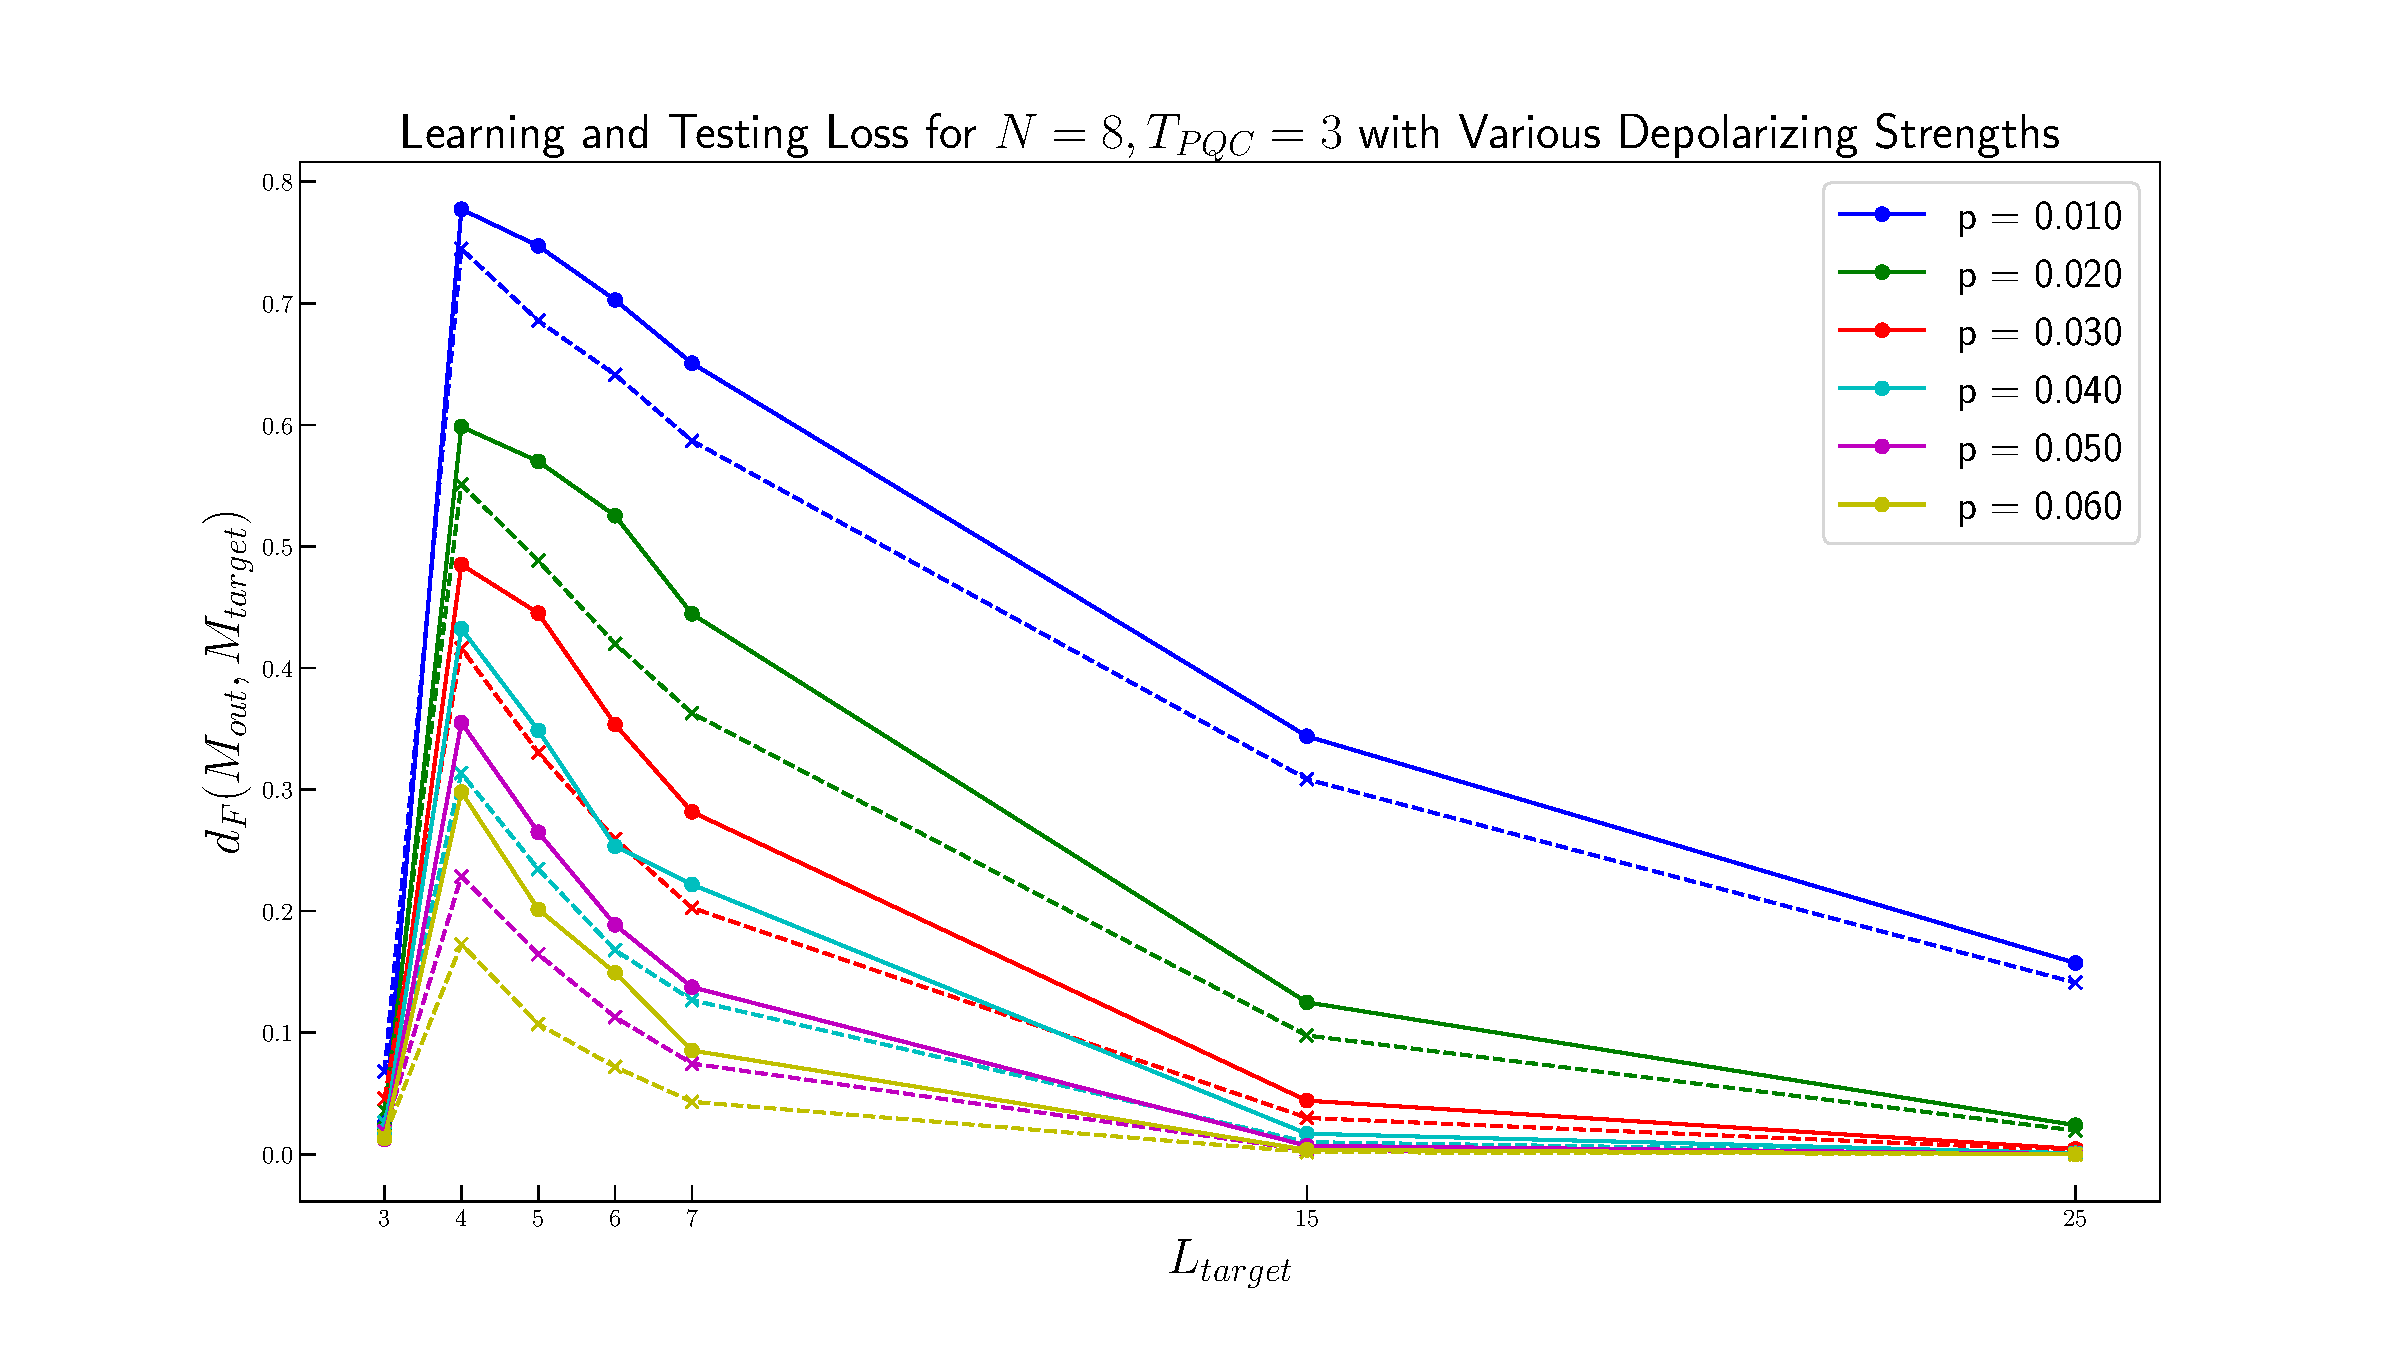
\includegraphics[width=\linewidth]{Depolarizing_ChangeT_N_L_p_8_3_all.pdf}
    \caption{}
    \label{fig:Depolarizing_ChangeT_N_L_p_8_3_all}
\end{subfigure}
\caption{\raggedright \yz{since we have many pauli strings with small weights, I suggest report the average loss conditioned on the input Pauli weight w, and normalize each loss by the target output norm.}The learning result of using a shallower PQC with $N=8$ qubits to learn a random $L_{target}$-layer PQC with various depolarizing noise. Solid lines represent the final average learning loss with all weight-1 Pauli strings, and dashed lines represent the final testing loss for 200 randomly sampled Pauli strings. Sub-figure \textbf{(a)} uses a 2-layer PQC, and Sub-figure \textbf{(b)} uses a 3-layer PQC.\yz{for all plots: fonts too small}}
\label{fig:Depolarizing_ChangeT_8}
\end{figure}

\begin{figure}
\centering
\begin{subfigure}{\linewidth}
    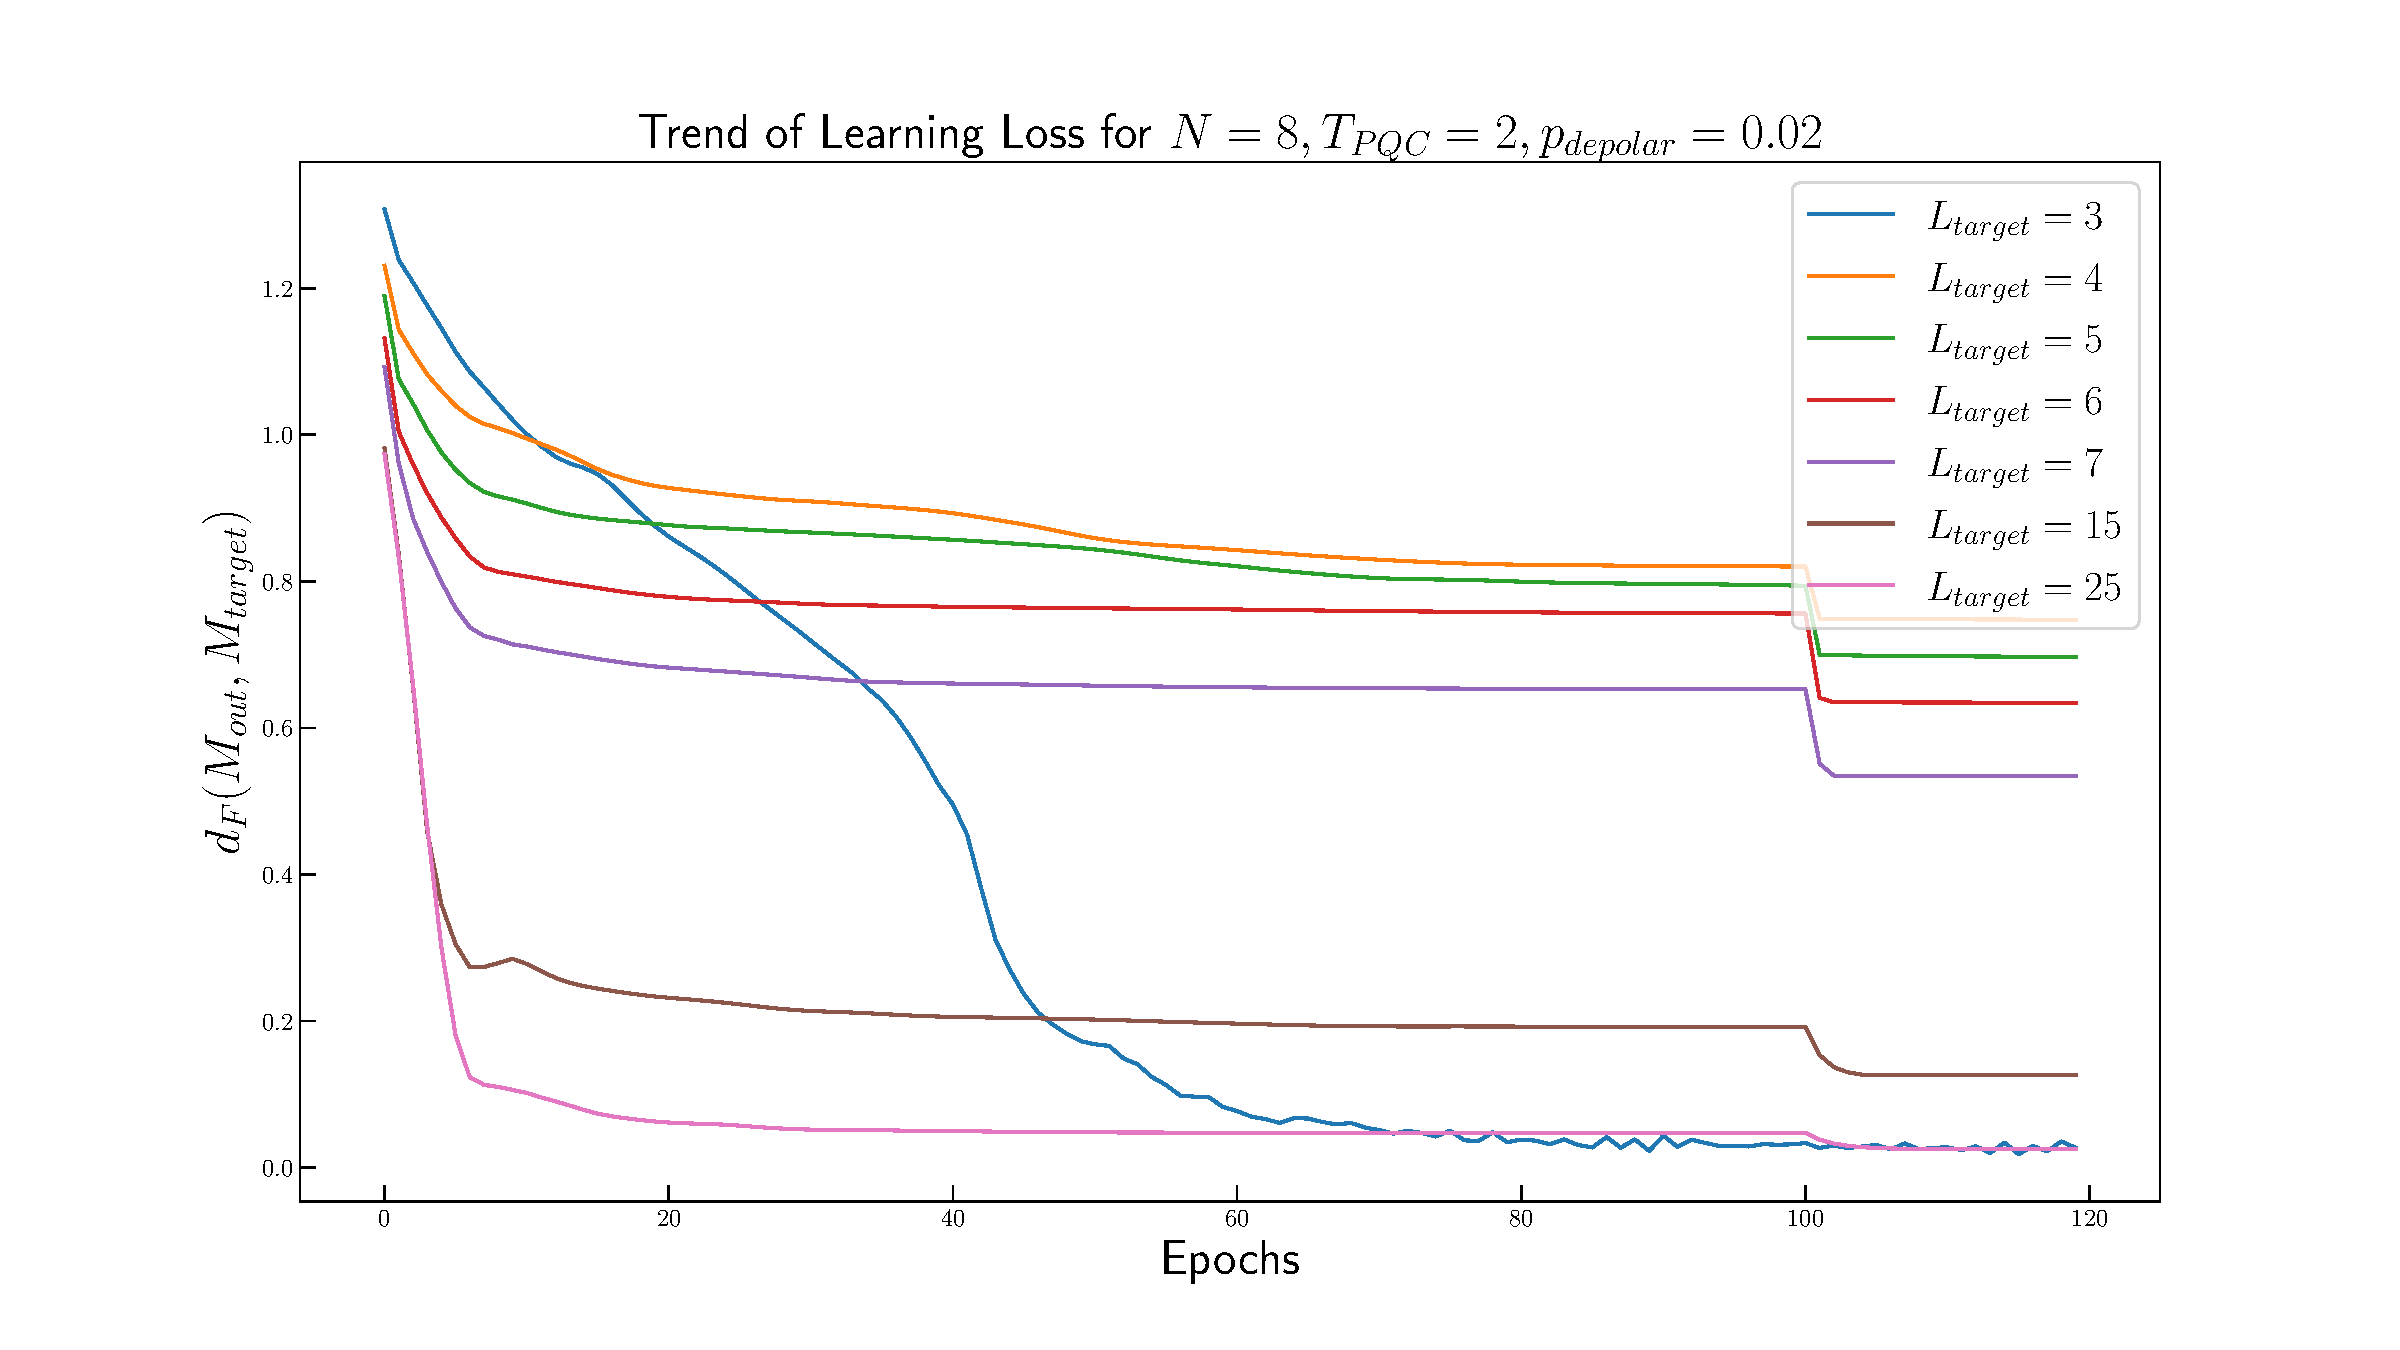
\includegraphics[width=\linewidth]{Depolarizing_learning_loss_trend_8_2_002.pdf}
    \caption{}
    \label{fig:Depolarizing_learning_loss_trend_8_2_002}
\end{subfigure}
\hfill
\begin{subfigure}{\linewidth}
    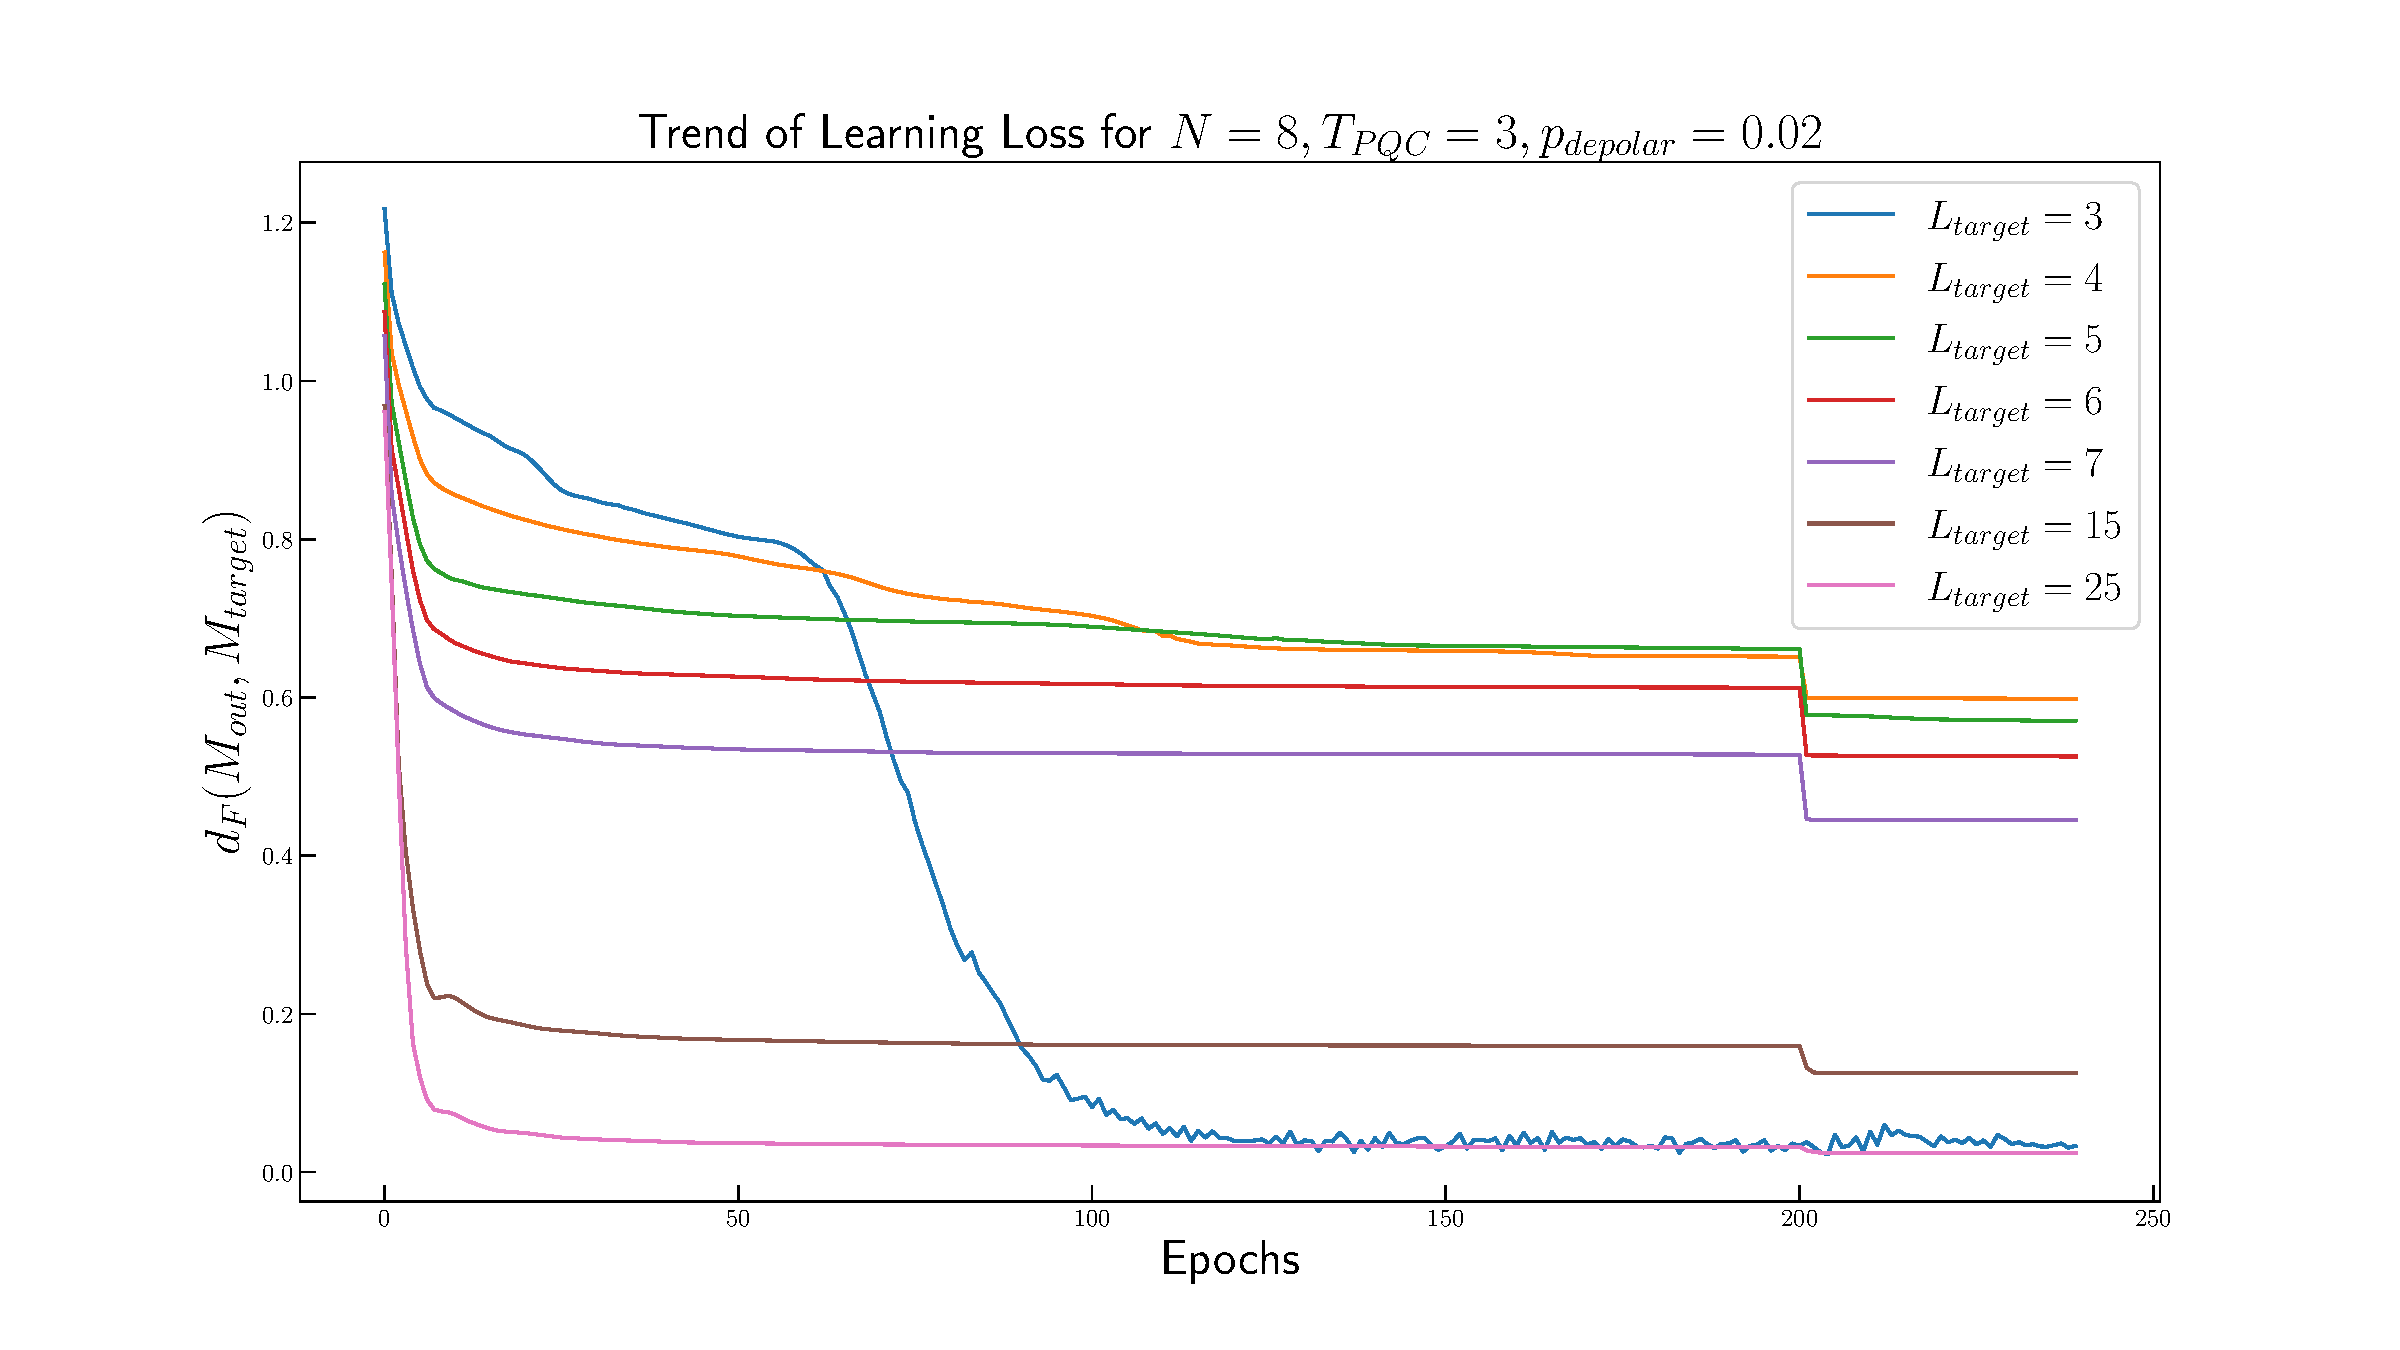
\includegraphics[width=\linewidth]{Depolarizing_learning_loss_trend_8_3_002.pdf}
    \caption{}
    \label{fig:Depolarizing_learning_loss_trend_8_3_002}
\end{subfigure}
\caption{\raggedright Example of the trend of the learning loss of using a shallower PQC to learn a random $L_{target}$-layer PQC with depolarizing probability $p_{depolar}=0.02$. Sub-figure \textbf{(a)} uses a 2-layer PQC and Sub-figure \textbf{(b)} uses a 3-layer PQC.}
\label{fig:Depolarizing_learning_loss_trend}
\end{figure}

Firstly, with the computational resources presented, the channel learning up to 8 qubits can be done without truncation. In Figure~\ref{fig:Depolarizing_ChangeT_8}, we demonstrated that using a 2-layer and a 3-layer PQC with moderate learning resources can effectively mimic a deeper circuit. The training is done with fewer than 200 epochs, and we notice that the convergence usually happens in the first 100 epochs. An example convergence training figure is shown in Figure~\ref{fig:Depolarizing_learning_loss_trend}. It is clear that when $T_{PQC}$ is smaller, it has faster convergence; however, all convergences are within a reasonable time, in about 200 epochs. 

The reason for the sudden drop in Figure~\ref{fig:Depolarizing_learning_loss_trend} at the final approximately $15\%$ of the training epochs is that, for the previous $85\%$, we restrict the maximum depolarizing noise in our model PQC to avoid the model getting stuck in a local minimum. If no restriction is imposed, the model PQC will quickly become a total depolarizing channel instead of learning the behaviours of the target channel.

\begin{figure}
\centering
\begin{subfigure}{\linewidth}
    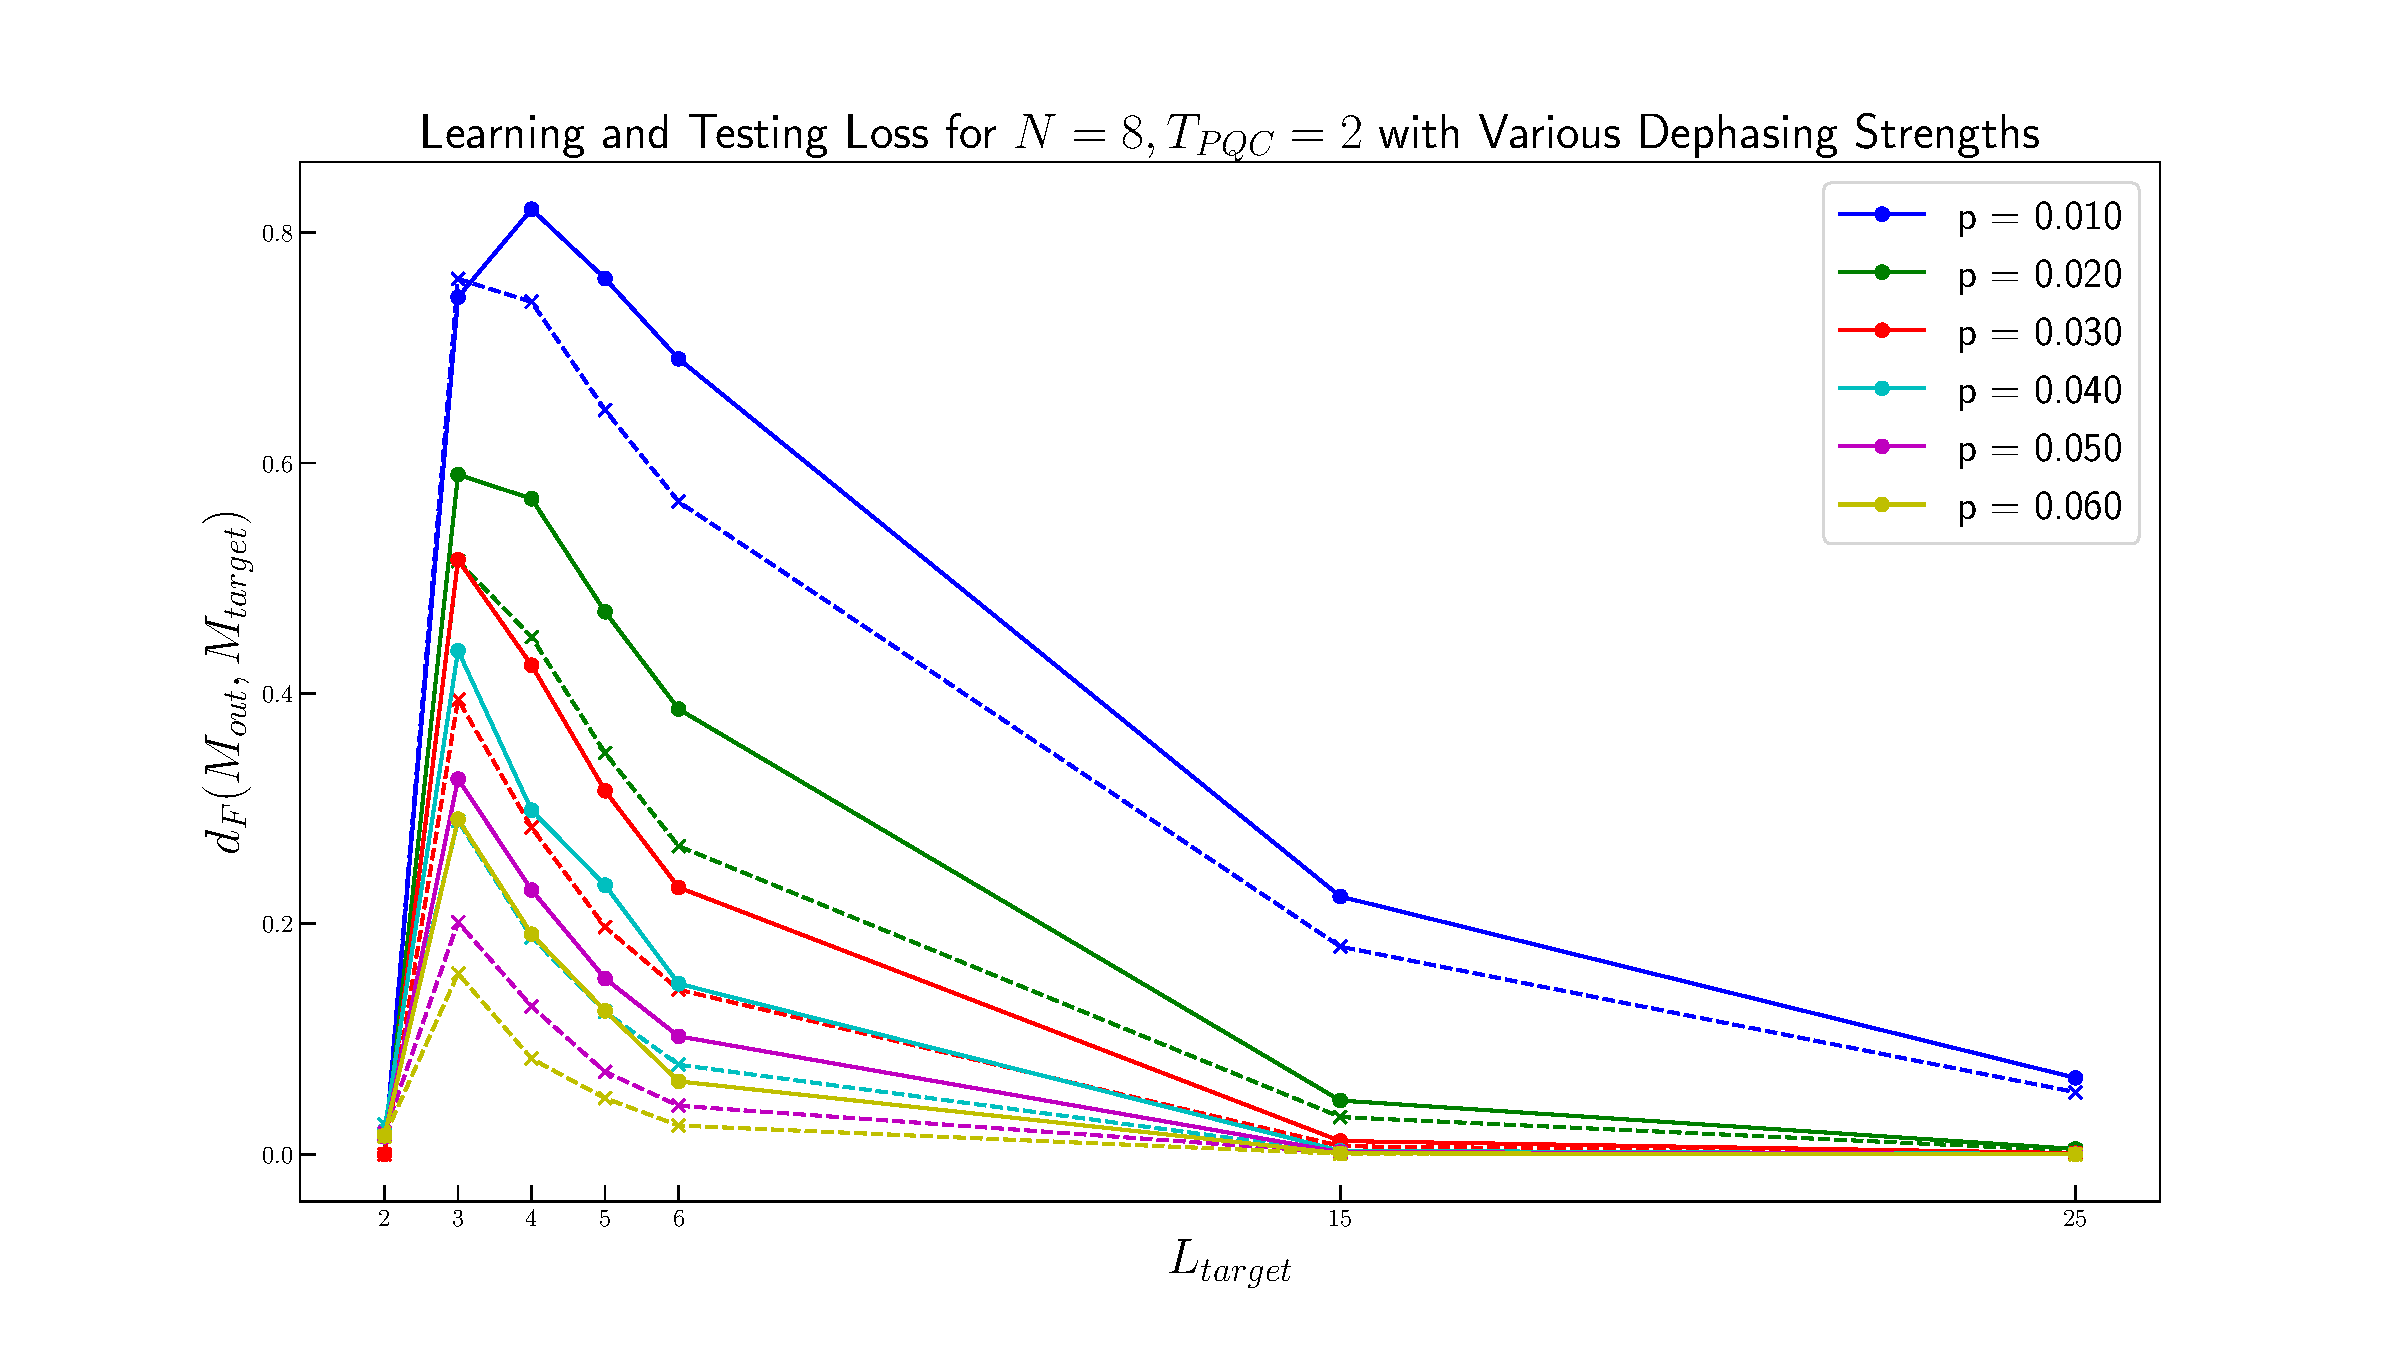
\includegraphics[width=\linewidth]{Dephasing_ChangeT_N_L_p_8_2_all.pdf}
    \caption{}
    \label{fig:Dephasing_ChangeT_N_L_p_8_2_all}
\end{subfigure}
\hfill
\begin{subfigure}{\linewidth}
    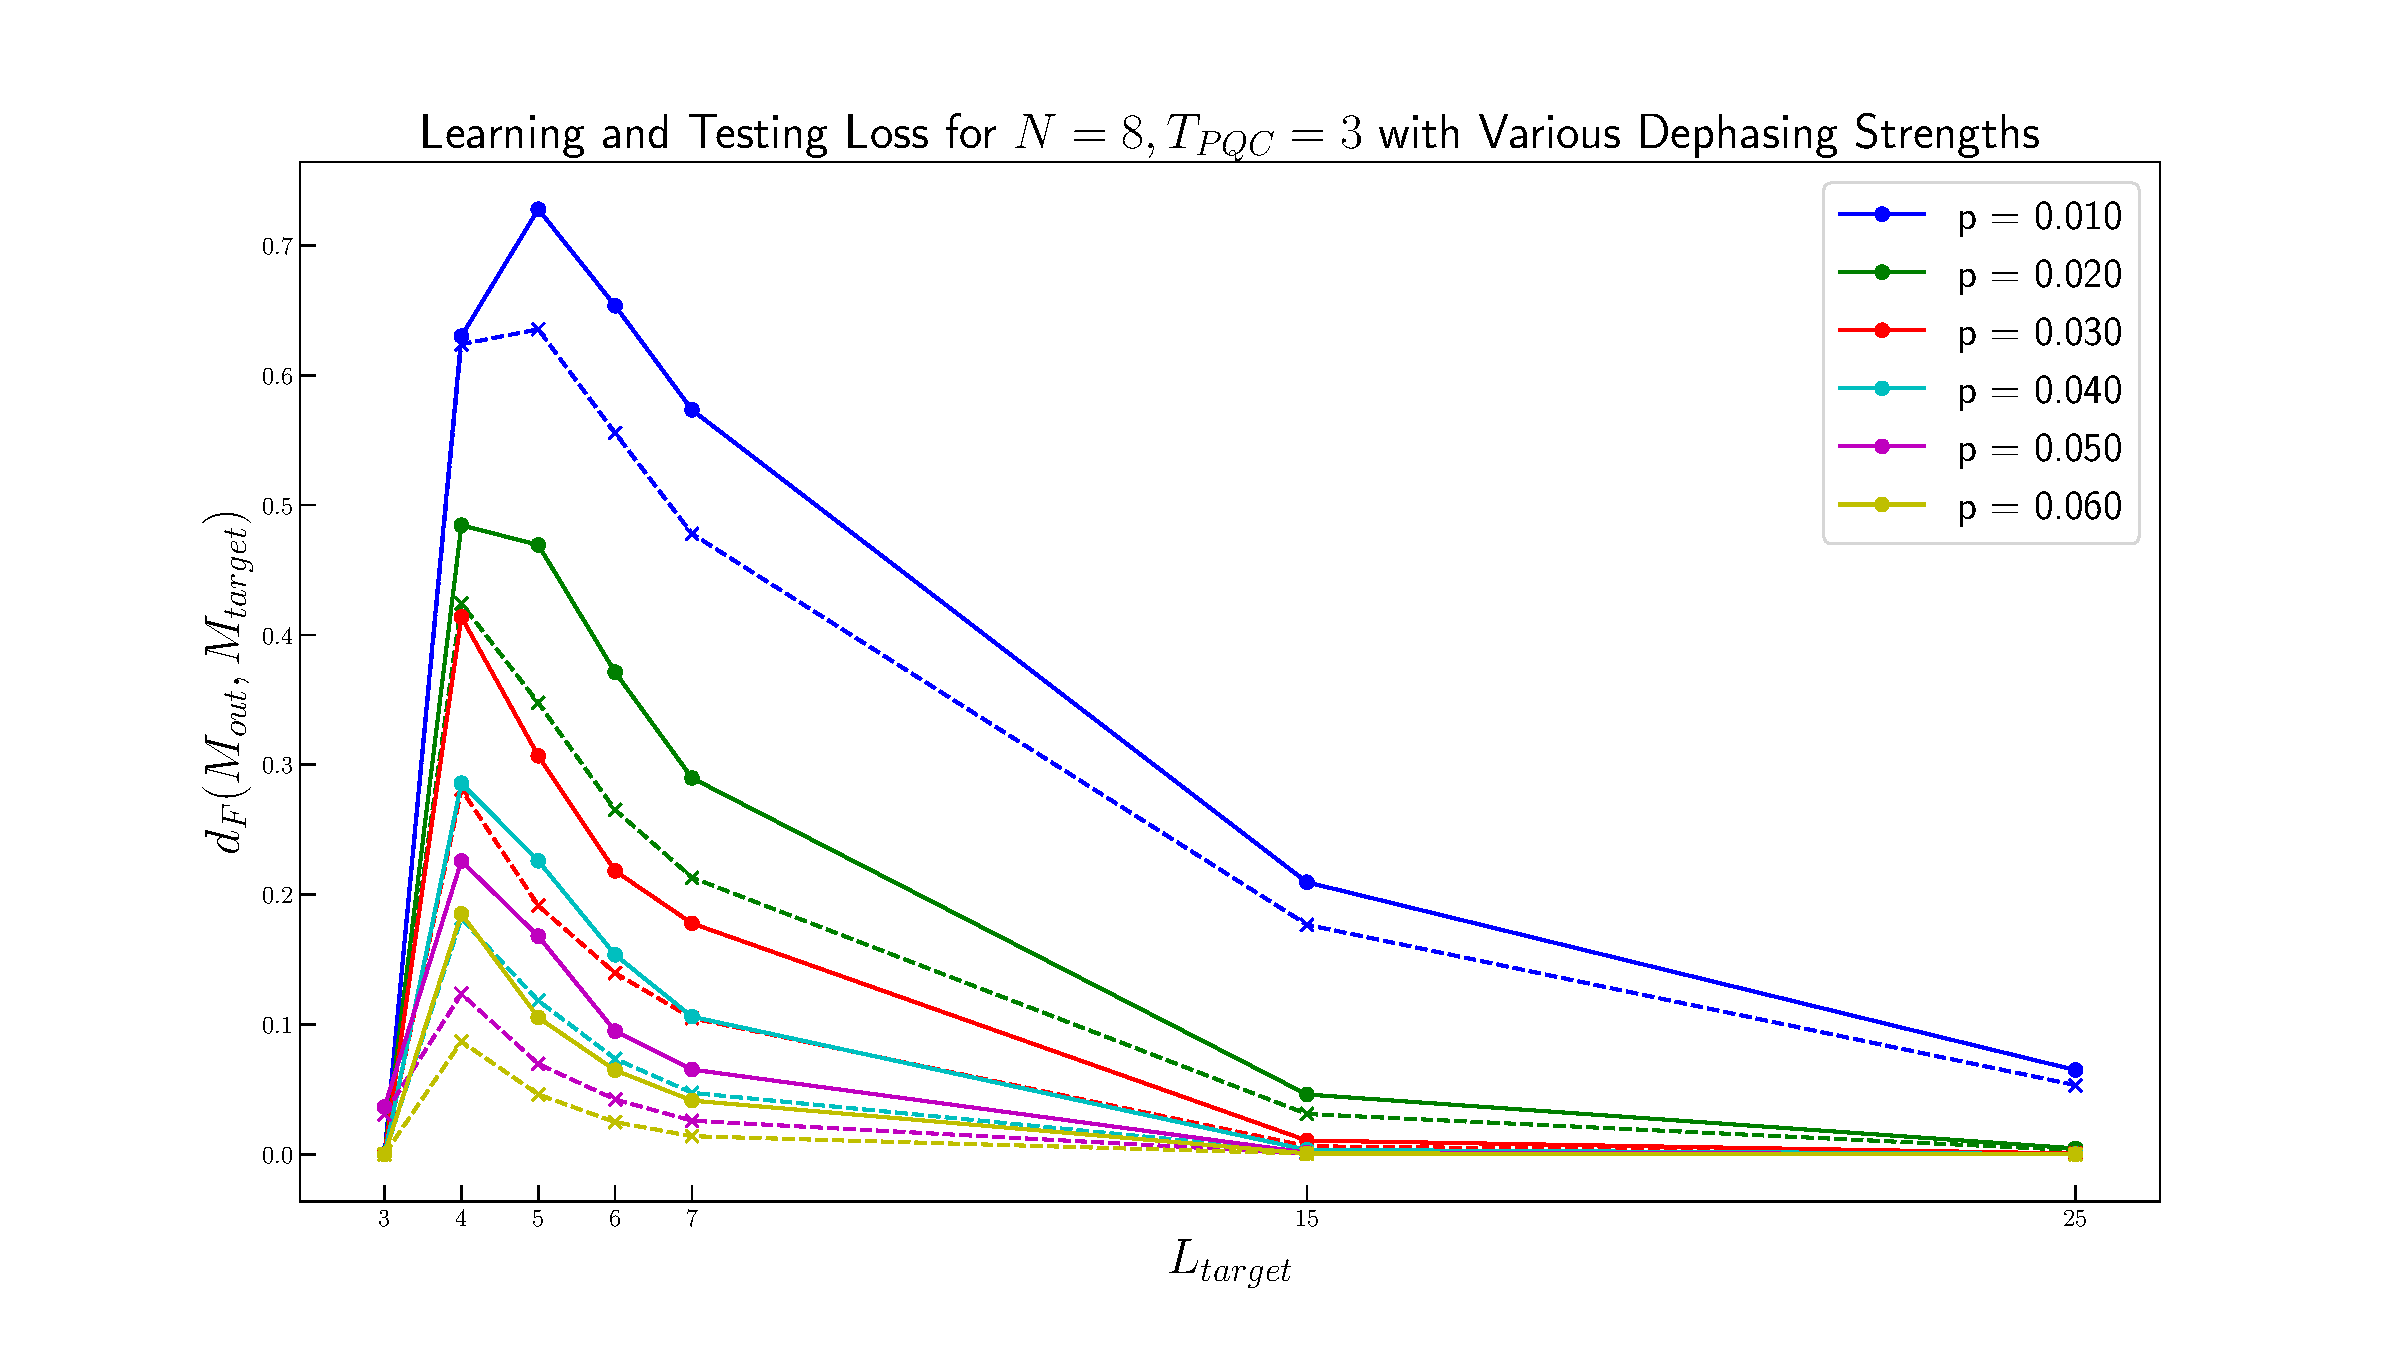
\includegraphics[width=\linewidth]{Dephasing_ChangeT_N_L_p_8_3_all.pdf}
    \caption{}
    \label{fig:Dephasing_ChangeT_N_L_p_8_3_all}
\end{subfigure}
\caption{\raggedright The learning result of using a shallower PQC with $N=8$ qubits to learn a random $L_{target}$-layer PQC with various dephasing noise. Solid lines represent the final average learning loss with all weight-1 Pauli strings, and dashed lines represent the final testing loss for 200 randomly sampled Pauli strings. Sub-figure \textbf{(a)} uses a 2-layer PQC, and Sub-figure \textbf{(b)} uses a 3-layer PQC.}
\label{fig:Dephasing_ChangeT_8}
\end{figure}

Similar learning results are obtained when we consider dephasing noise in the channel. Results are shown in Figure~\ref{fig:Dephasing_ChangeT_8}, where effective compression of a dephasing channel is possible, which significantly reduces the computational resources required for computation.

We emphasize that the above results are obtained without any truncation, ensuring their accuracy. 

\subsection{Compressing a Quantum Circuit with 12 sites}

\begin{figure}
\centering
\begin{subfigure}{\linewidth}
    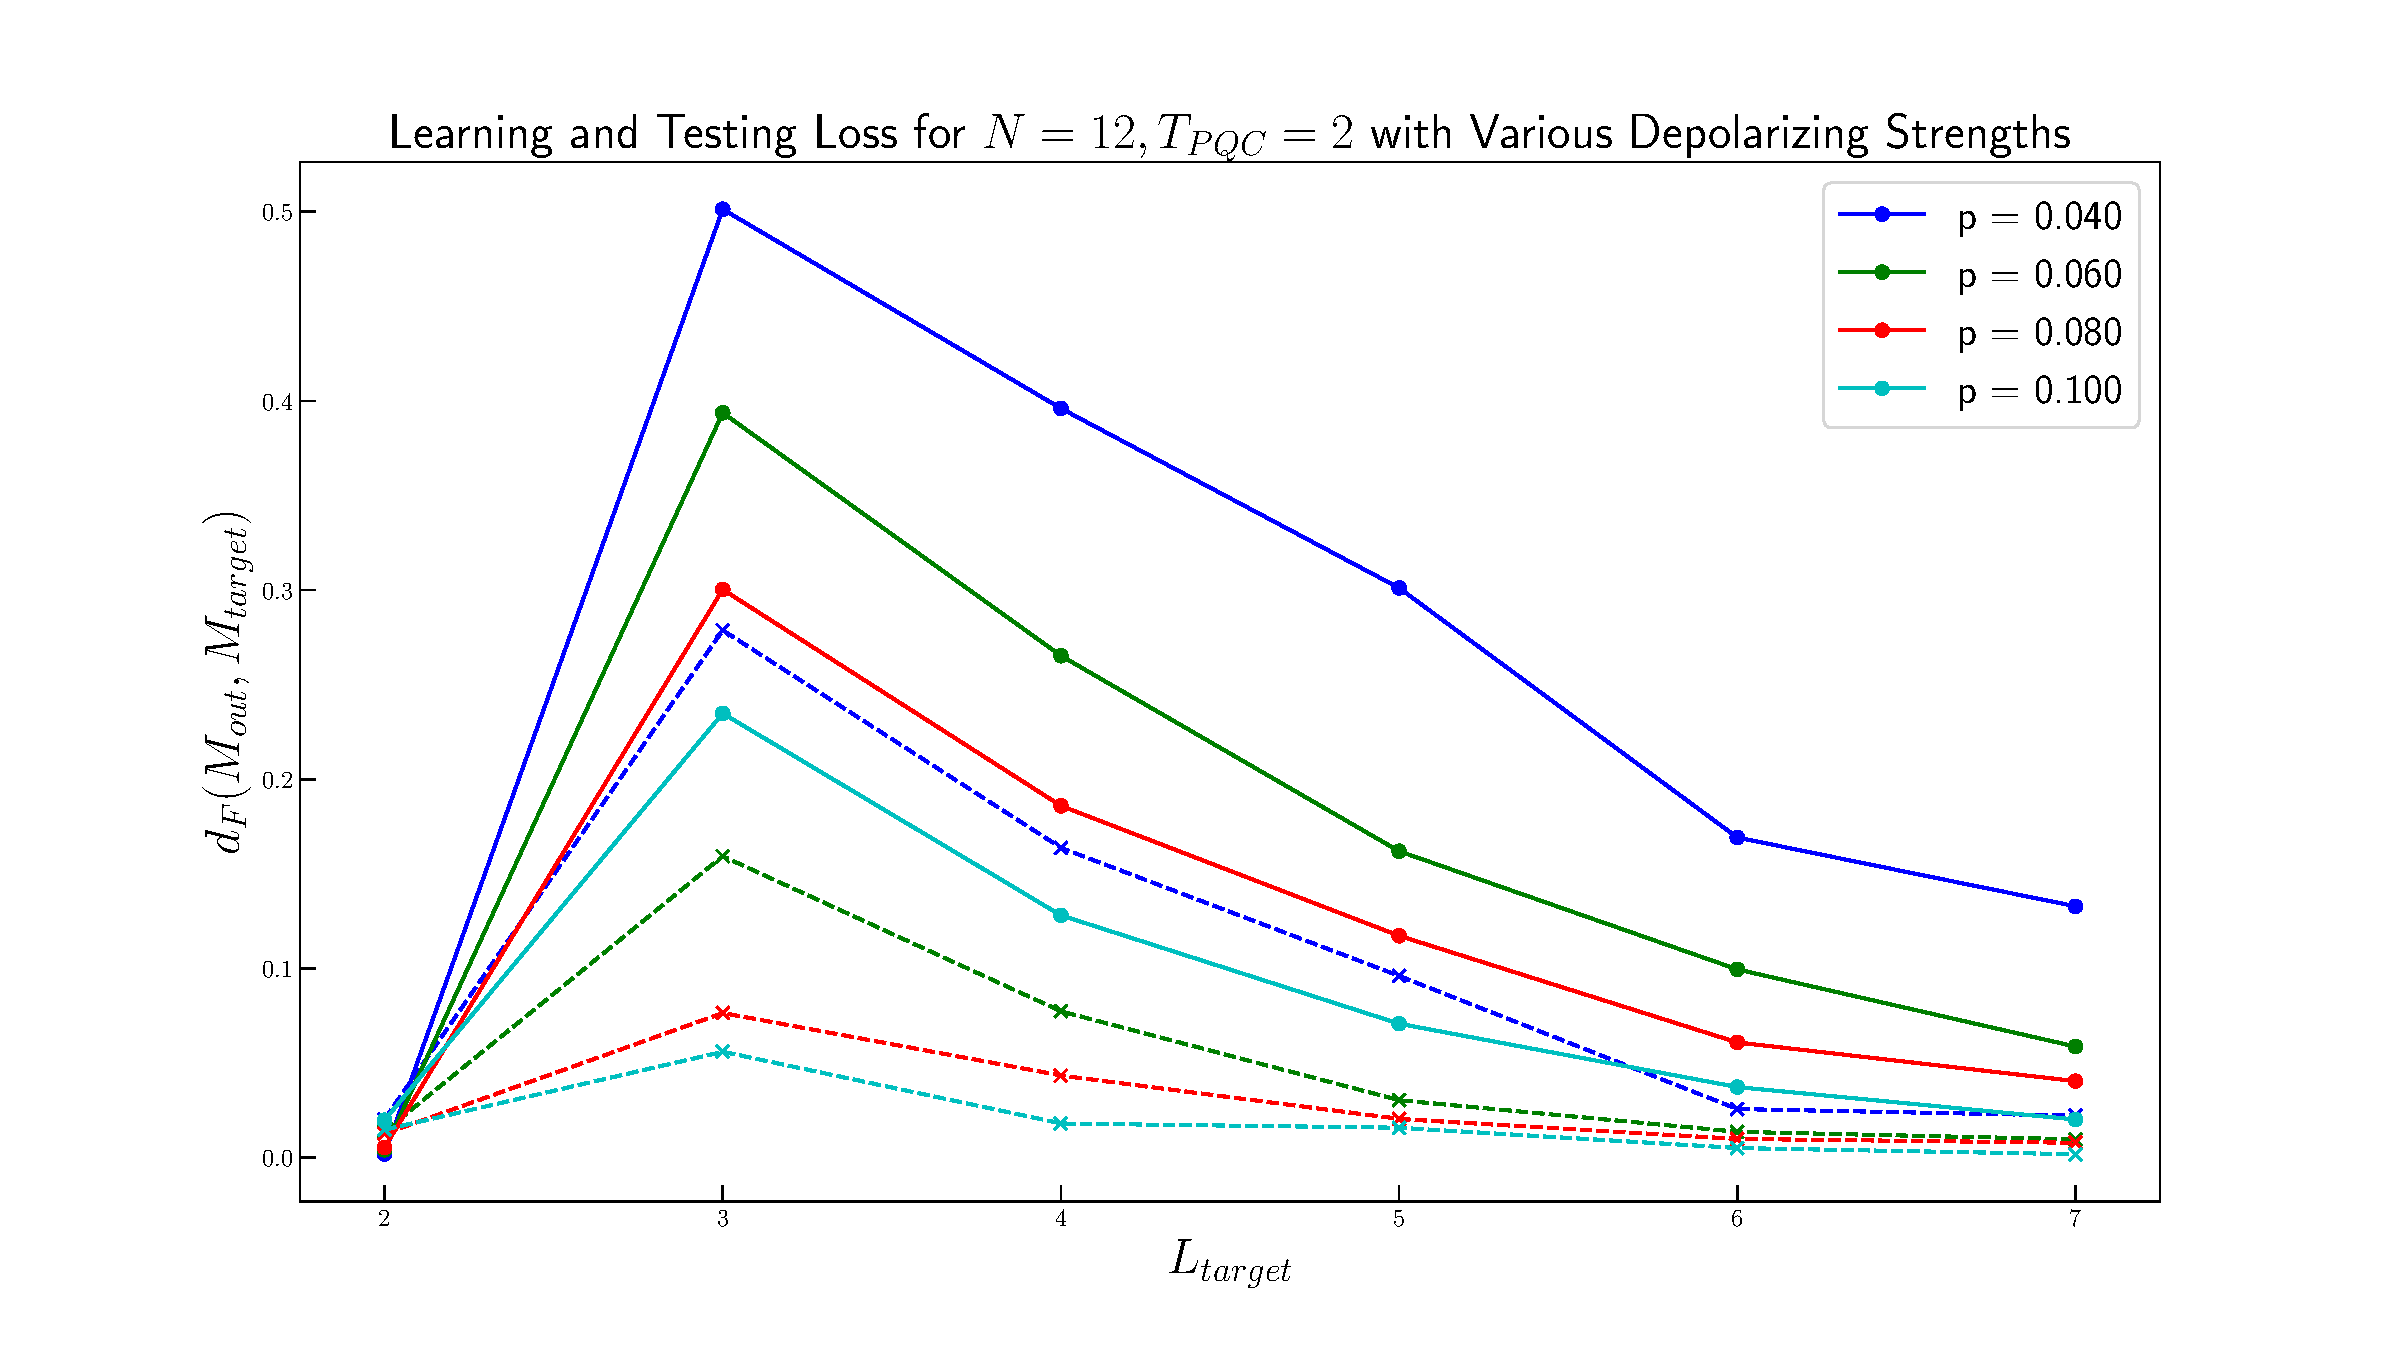
\includegraphics[width=\linewidth]{Depolarizing_ChangeT_N_L_p_12_2_all.pdf}
    \caption{}
    \label{fig:Depolarizing_ChangeT_N_L_p_12_2_all}
\end{subfigure}
\hfill
\begin{subfigure}{\linewidth}
    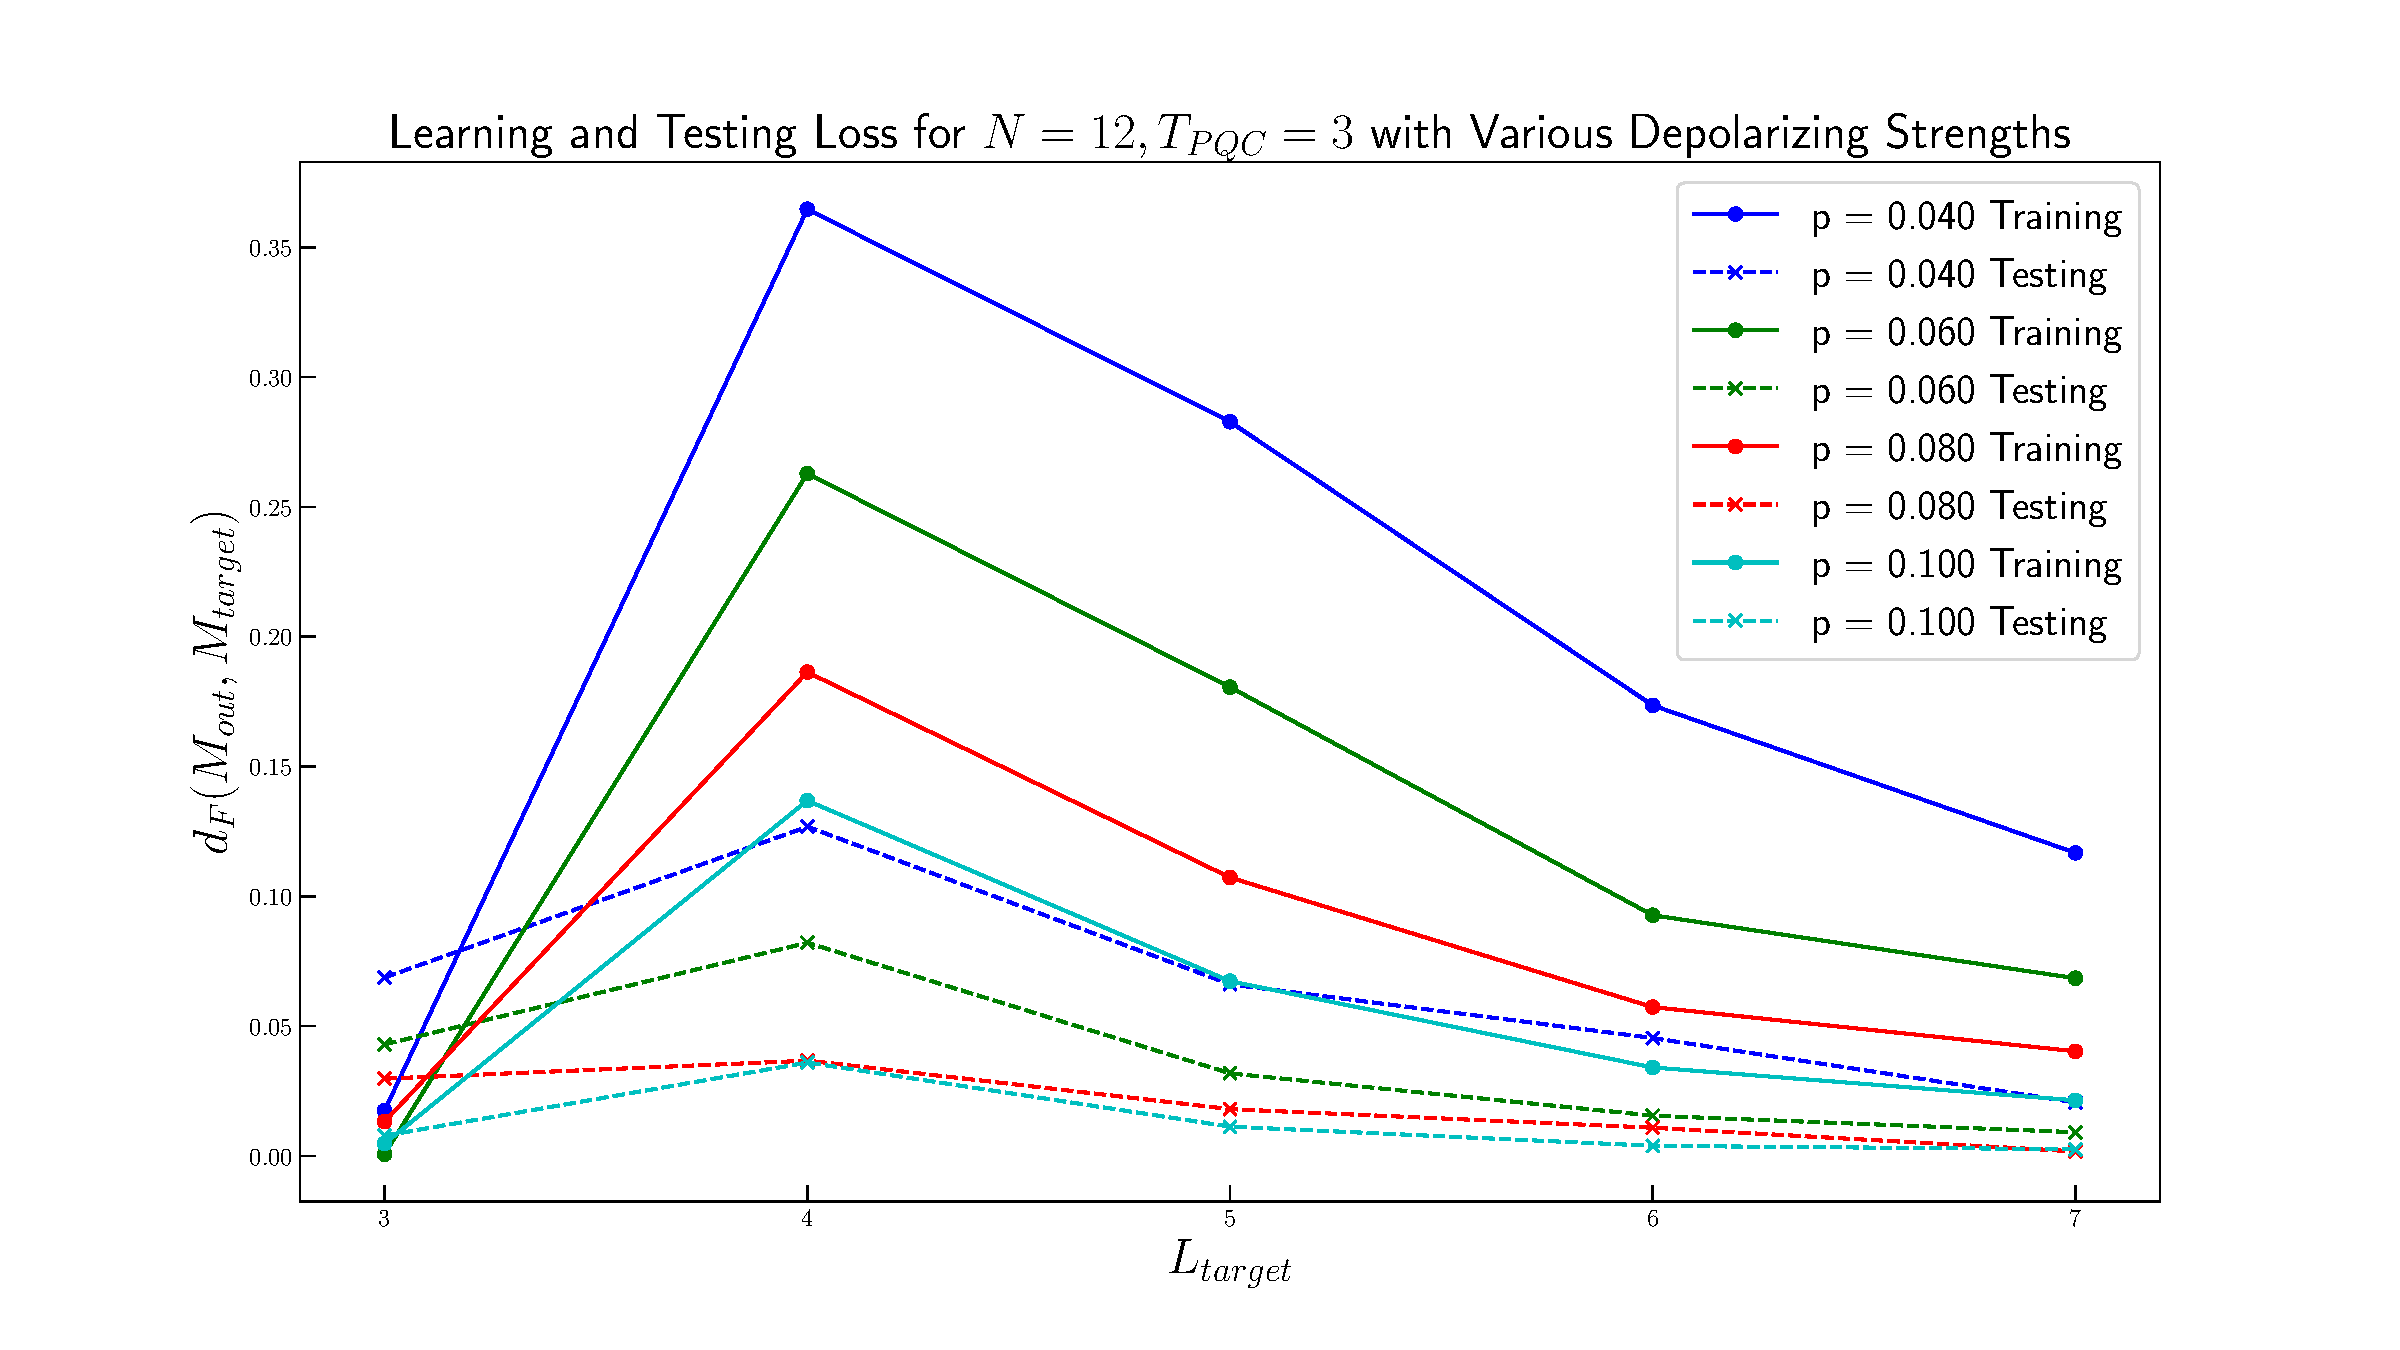
\includegraphics[width=\linewidth]{Depolarizing_ChangeT_N_L_p_12_3_all.pdf}
    \caption{}
    \label{fig:Depolarizing_ChangeT_N_L_p_12_3_all}
\end{subfigure}
\caption{\raggedright The learning result of using a shallower PQC with $N=12$ qubits with truncation $d_{max}=64, \epsilon_{cutoff}=10^{-5}$ to learn a random $L_{target}$-layer PQC with various depolarizing noise. Solid lines represent the final average learning loss with all weight-1 Pauli strings, and dashed lines represent the final testing loss for 200 randomly sampled Pauli strings. Sub-figure \textbf{(a)} uses a 2-layer PQC, and Sub-figure \textbf{(b)} uses a 3-layer PQC.}
\label{fig:Depolarizing_ChangeT_12}
\end{figure}

When propagating Pauli strings as an MPS through a general PQC, the bond dimension will grow exponentially with the depth and the number of qubits in the system. Therefore, truncation is needed for efficient learning. 

In our architecture, truncation is implemented by cutting the MPS bond dimensions after each layer of gates. We use the SVD algorithm to perform the canonicalization of the MPS. When computing the SVD of each MPS site, we set a threshold on the maximum bond dimension $d_{max}$ kept and a cutoff singular value $\epsilon_{cutoff}$. For a bond between 2 MPS sites, all singular values below the cutoff $\epsilon_{cutoff}$ will be discarded. Then, if the bond dimension is still greater than the maximum bond dimension $d_{max}$, only the largest $d_{max}$ singular values at each bond will be kept.

\begin{figure}
    \centering
    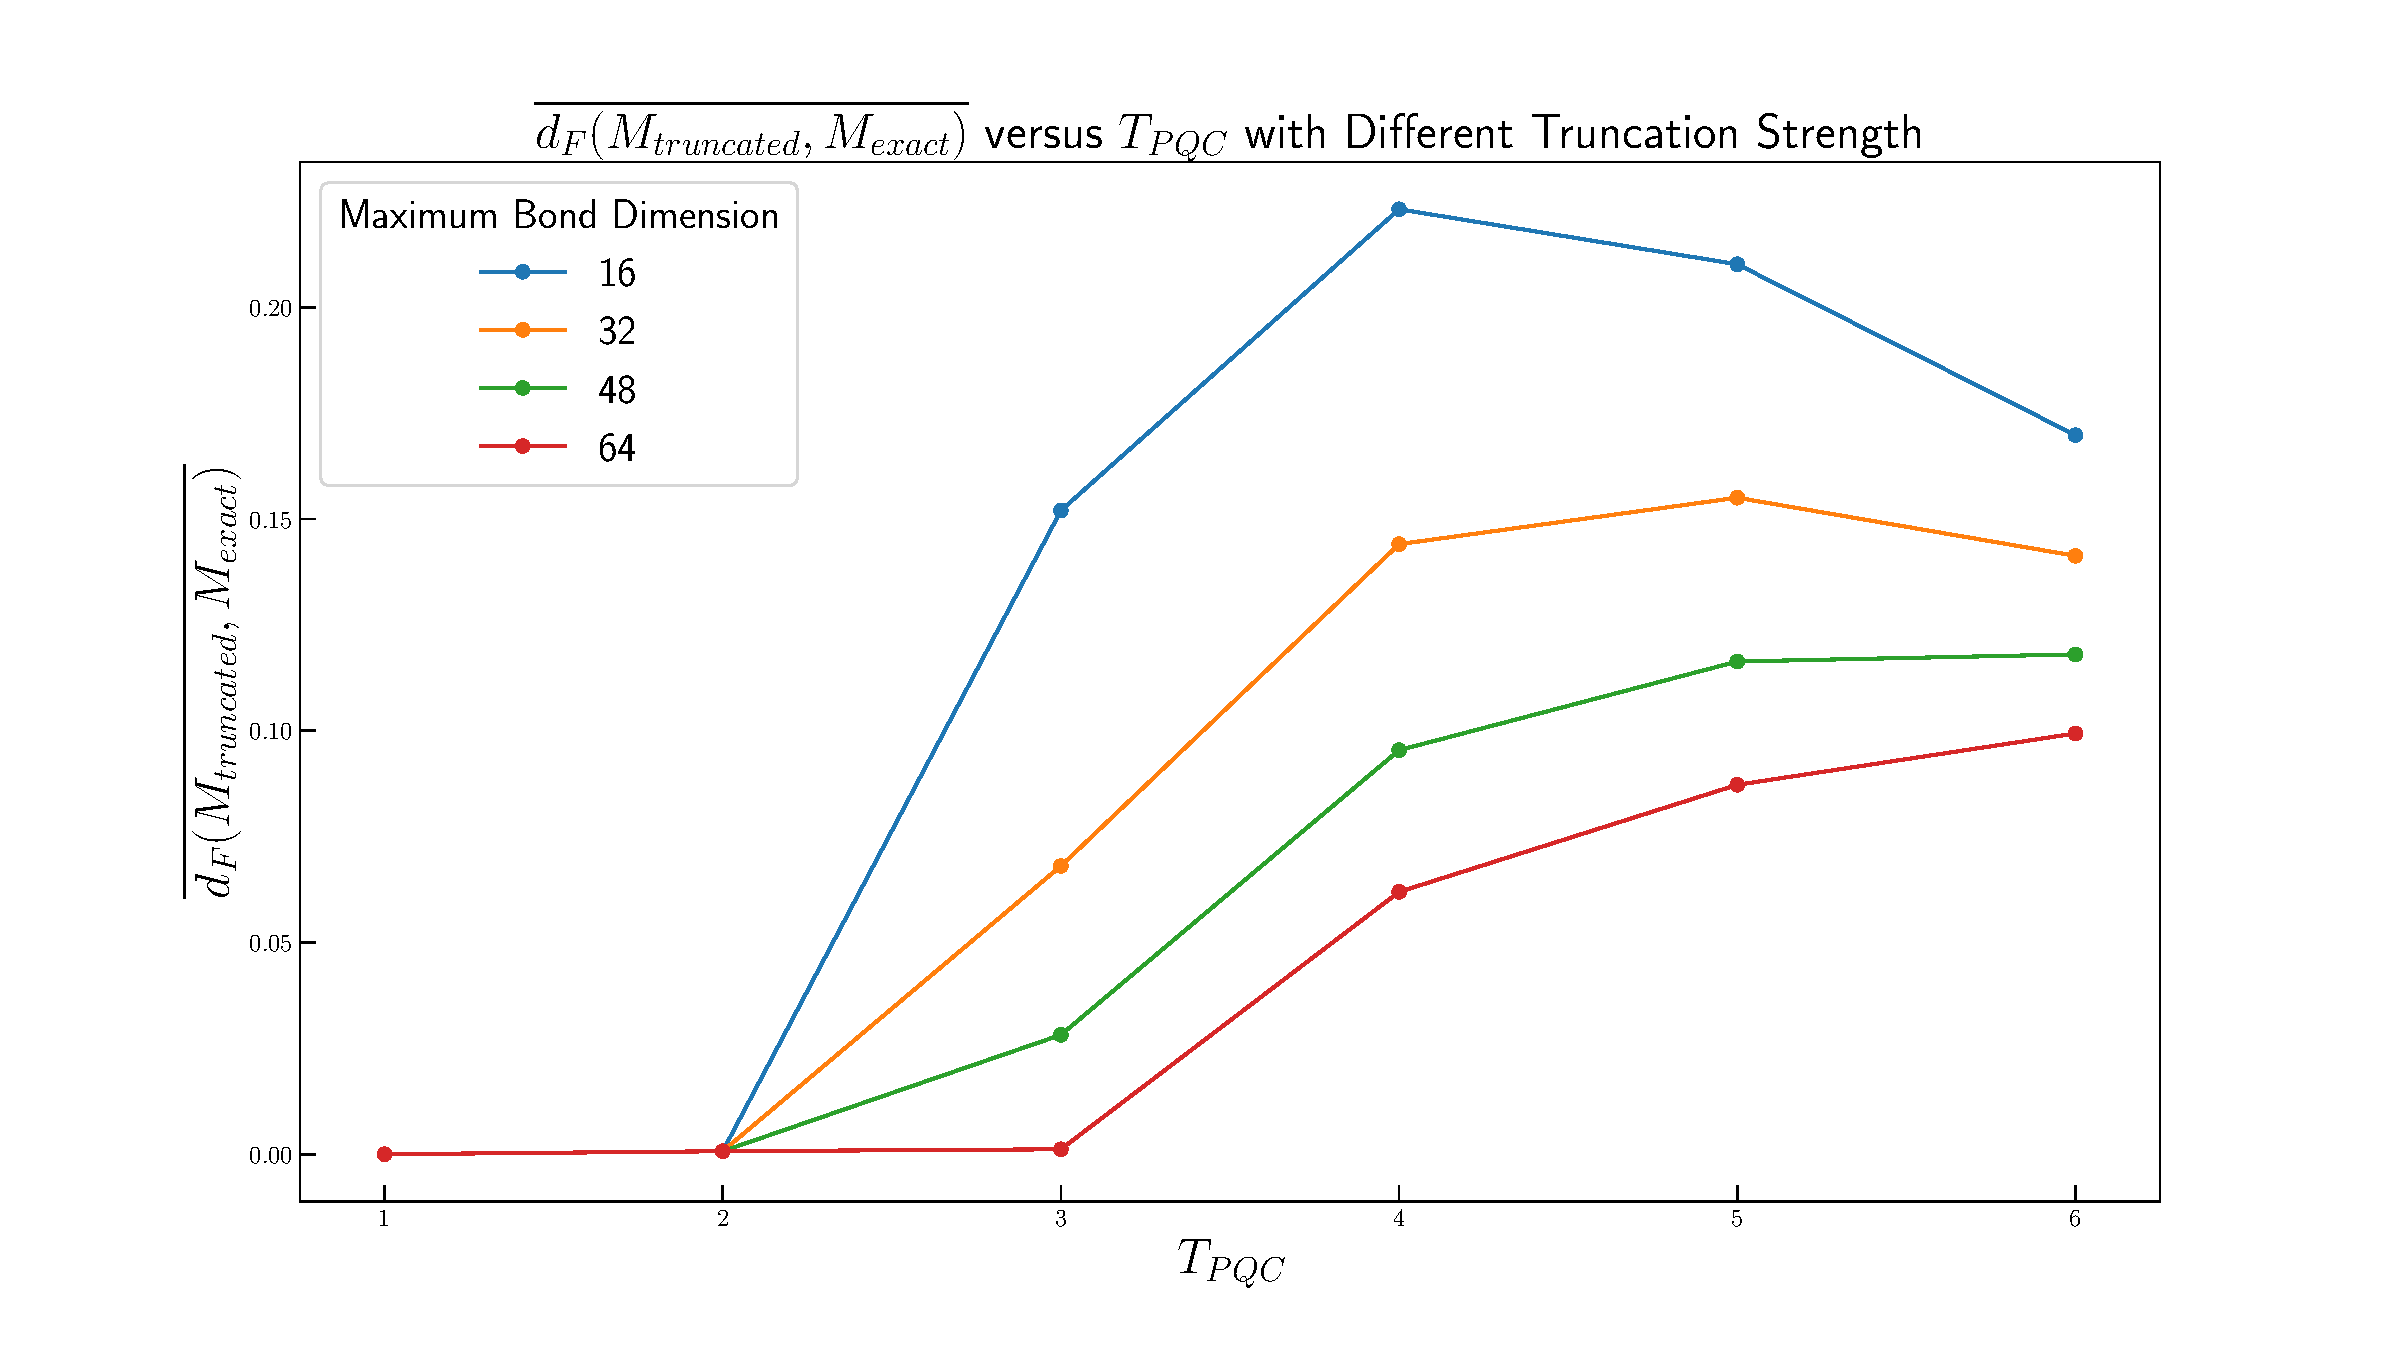
\includegraphics[width=\linewidth]{Truncation_error_N_12.pdf}
    \caption{\raggedright The average Frobenius distance between passing through a weight-1 Pauli string through a $T_{PQC}$ layer PQC with and without truncation, with depolarizing noise $p=0.04$. \yijian{Not seen convergence with bond dimension?} \simba{I do not fully understand this comment.}}
    \label{fig:Truncation_error_N_12}
\end{figure}

However, when performing PQC learning without non-unitary noise, truncation typically leads to significant error. However, with small non-unitary noise, the small singular values at each MPS bond are significantly suppressed, and the truncation error becomes tolerable. 

In Figure~\ref{fig:Truncation_error_N_12}, we have shown an example of the average truncation error obtained when passing a weight-1 Pauli string through a $T_{PQC}$ layer PQC model at a depolarizing noise strength of $p=0.04$. Denote the truncated final MPS by $M_{truncated}$ and the exact final MPS by $M_{exact}$. Figure~\ref{fig:Truncation_error_N_12} shows the mean Frobenius distance $\overline{d_F(M_{truncated}, M_{exact})}$ between the two MPS, averaged over all 36 initial weight-1 Pauli strings. Clearly, the higher the maximum bond dimension, the smaller the distance, but it also requires more computational resources. The dropping trend of the Frobenius distance is due to the depolarizing noise applied to the system.

In this subsection, we truncate the bond dimension of the MPS to $d_{max}=64$ and set $\epsilon_{cutoff}=10^{-5}$. To avoid significant truncation error, we set the lowest depolarizing probability for learning to $p_{depolar}=0.04$ and obtain a similar result.

Figure~\ref{fig:Depolarizing_ChangeT_12} shows the learning result of using a shallower PQC with $N=12$ qubits with truncation $d_{max}=64, \epsilon_{cutoff}=10^{-5}$ to learn a random $L_{target}$-layer PQC with various depolarizing noise. The general trend is the same as in the case of $N=8$ qubits. Therefore, we believe the results are general and can be applied to a larger number of qubits.


\subsection{Compressing a Quantum Circuit with 30 sites}

\begin{figure}
    \centering
    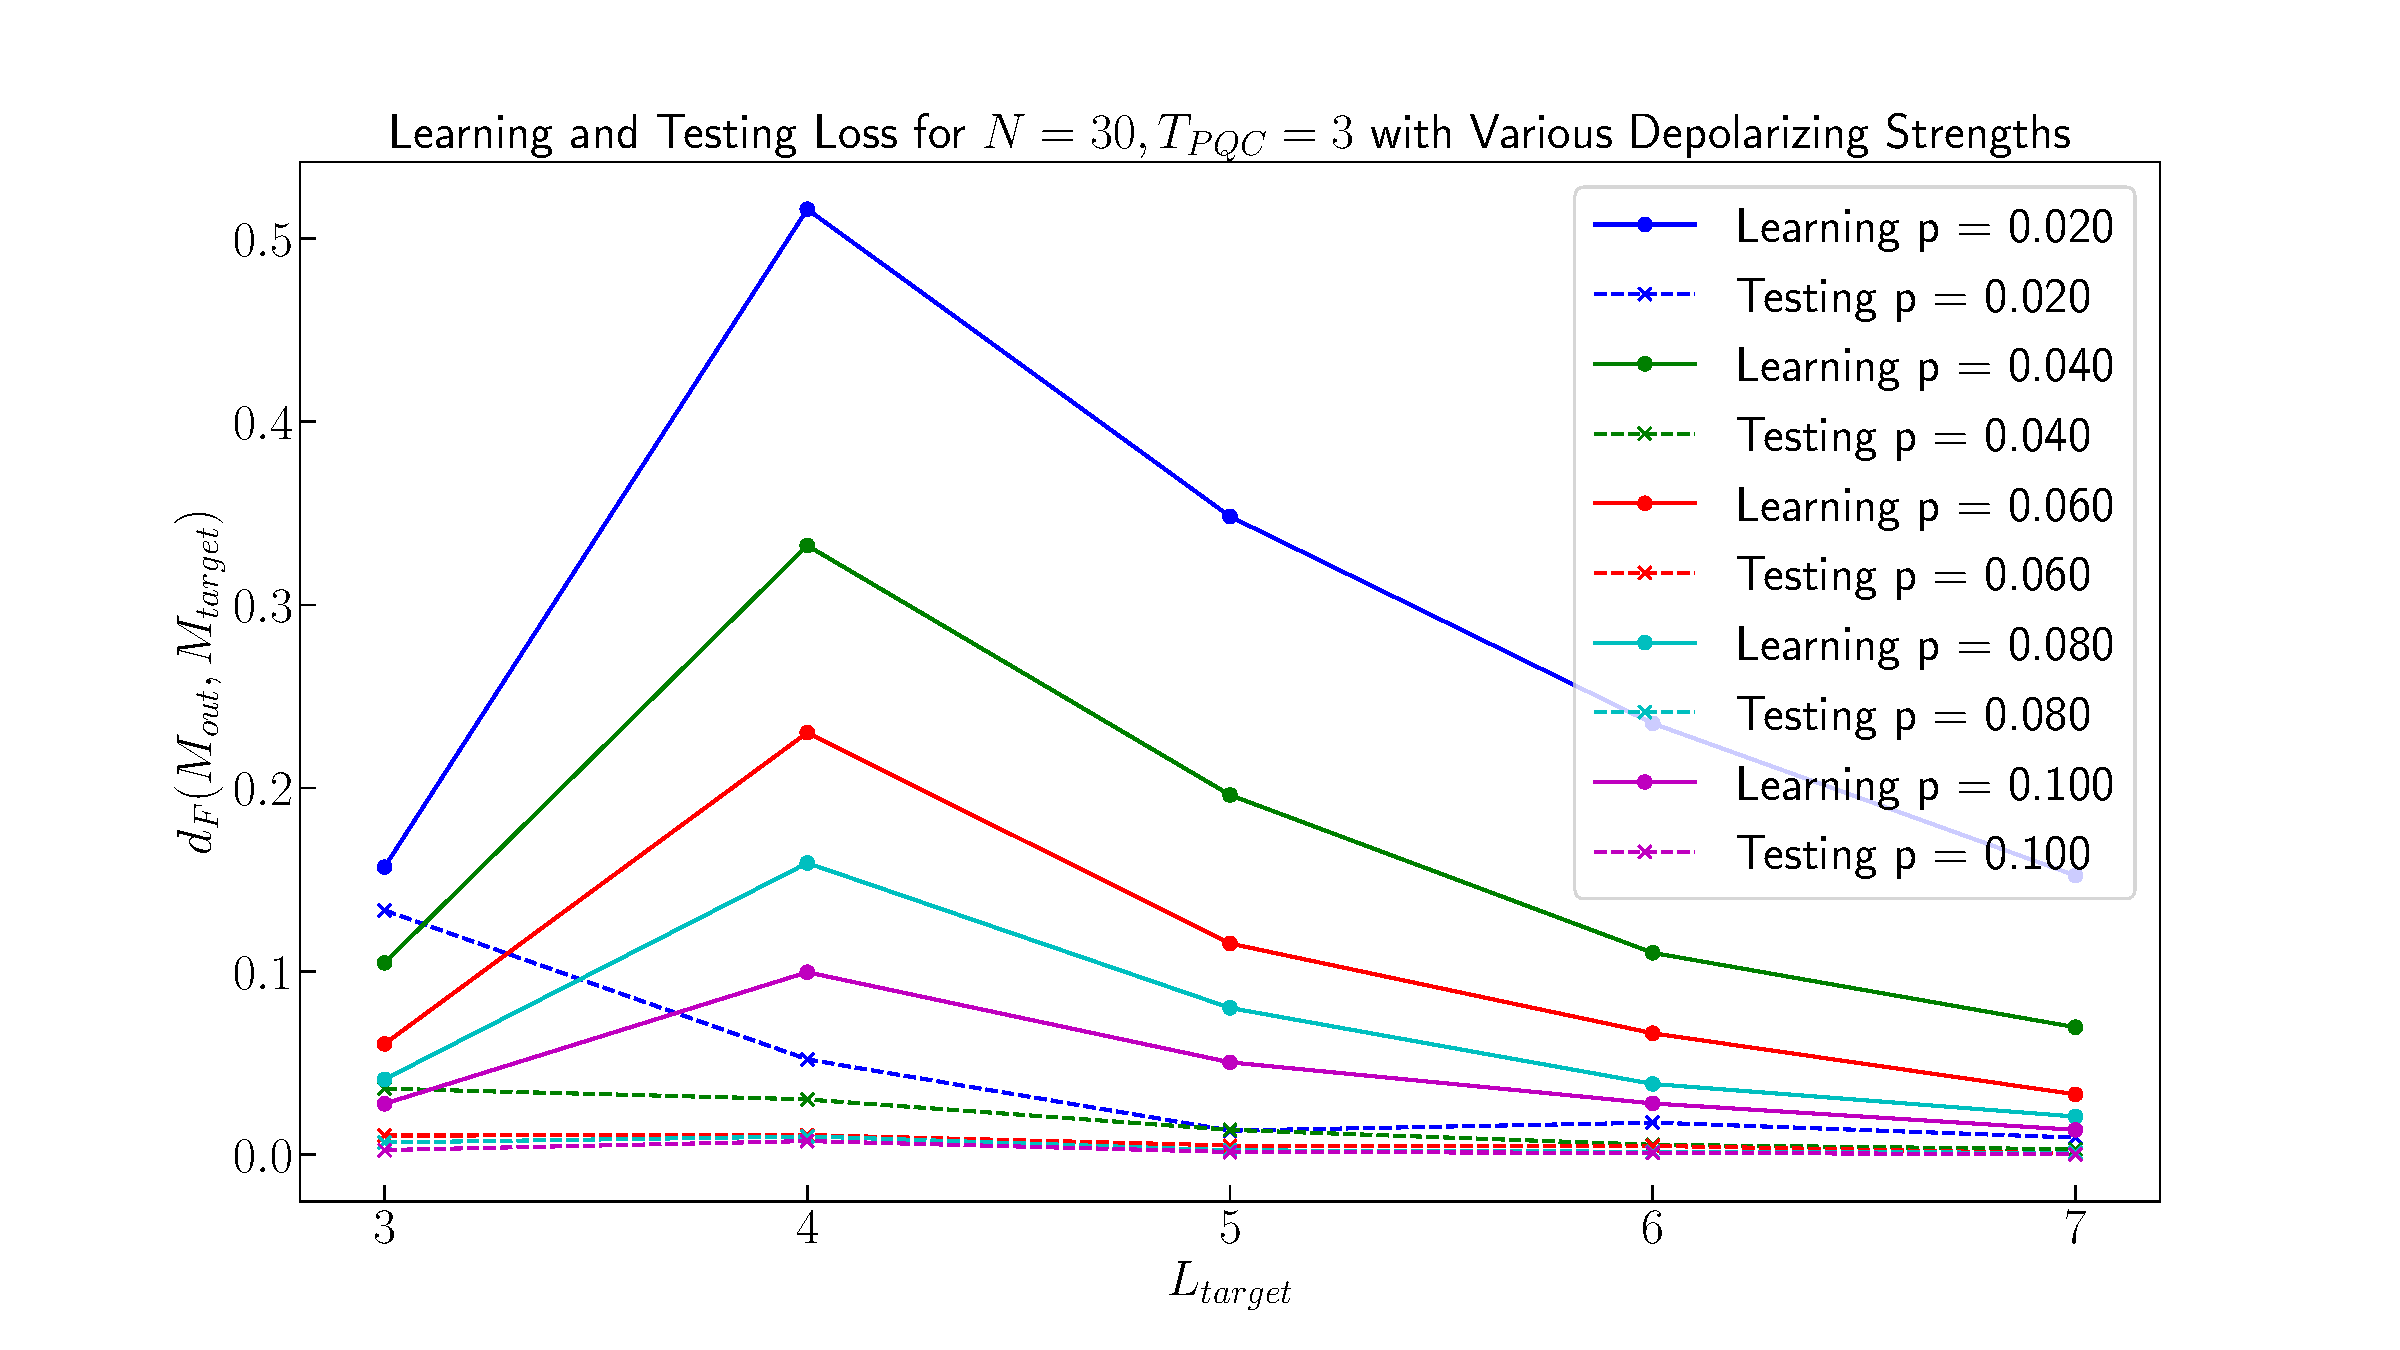
\includegraphics[width=\linewidth]{Depolarizing_ChangeT_N_L_p_30_3_all.pdf}
    \caption{\raggedright The learning result of using a shallower PQC with $N=30$ qubits with truncation $d_{max}=32, \epsilon_{cutoff}=10^{-5}$ to learn a random $L_{target}$-layer PQC with various depolarizing noise. Solid lines represent the final average learning loss with all weight-1 Pauli strings, and dashed lines represent the final testing loss for 200 randomly sampled Pauli strings.}
    \label{fig:Depolarizing_ChangeT_N_L_p_30_3_all}
\end{figure}
The above results of learning quantum circuits for 8 and 12 sites are all runnable on local user-grade computers. To demonstrate the power of our code, we tried running our code on a normal computational CPU cluster; with that, we are able to learn and compress quantum circuits with over 30 sites with truncation. The result is shown in Figure~\ref{fig:Depolarizing_ChangeT_N_L_p_30_3_all}, where we see the same general trend as the learning with a smaller number of qubit sites. However, the testing loss in this case is generally much lower than the learning loss. The reason is discussed in Section~\ref{sec:Training_dataset_generation}, that the training phase is done using all weight-1 Pauli strings, and testing is done with random weight Pauli strings. The higher the testing weight of the Pauli string, the more mixed the final state is. Therefore, when the system only consists of 8 or 12 qubit sites, the final state is not very mixed, which shows traces of difference, and for 30 qubit case, the final state eventually become very mixed. Thus, the testing loss appears to be very low.



\subsection{Quantum Channel Learning with small depolarizing noise}
\label{sec:Numerical_result_Lindbladian}

We demonstrated that the learning can be efficiently done with a small error rate per layer, specifically, if we add a per-layer depolarizing noise $p$ of a few percent, the learning can be done efficiently. While in most of the previous plots, if we use a $T_{PQC}$-layer, $T_{PQC}=2, 3$, PQC to learn a Haar random $L_{target}$-layer PQC, then usually the learning and testing loss will peak at $L_{target}=T_{PQC}+1$. Because, for $L_{target}=T_{PQC}$, the complexity of the model and the target circuits are the same, which means the model PQC should be able to learn the target PQC perfectly, and for $L_{target}\ge T_{PQC}+2$, the depolarizing or dephasing noise will override, and the learning loss will be reduced.

\begin{figure}
\centering
\begin{subfigure}{\linewidth}
    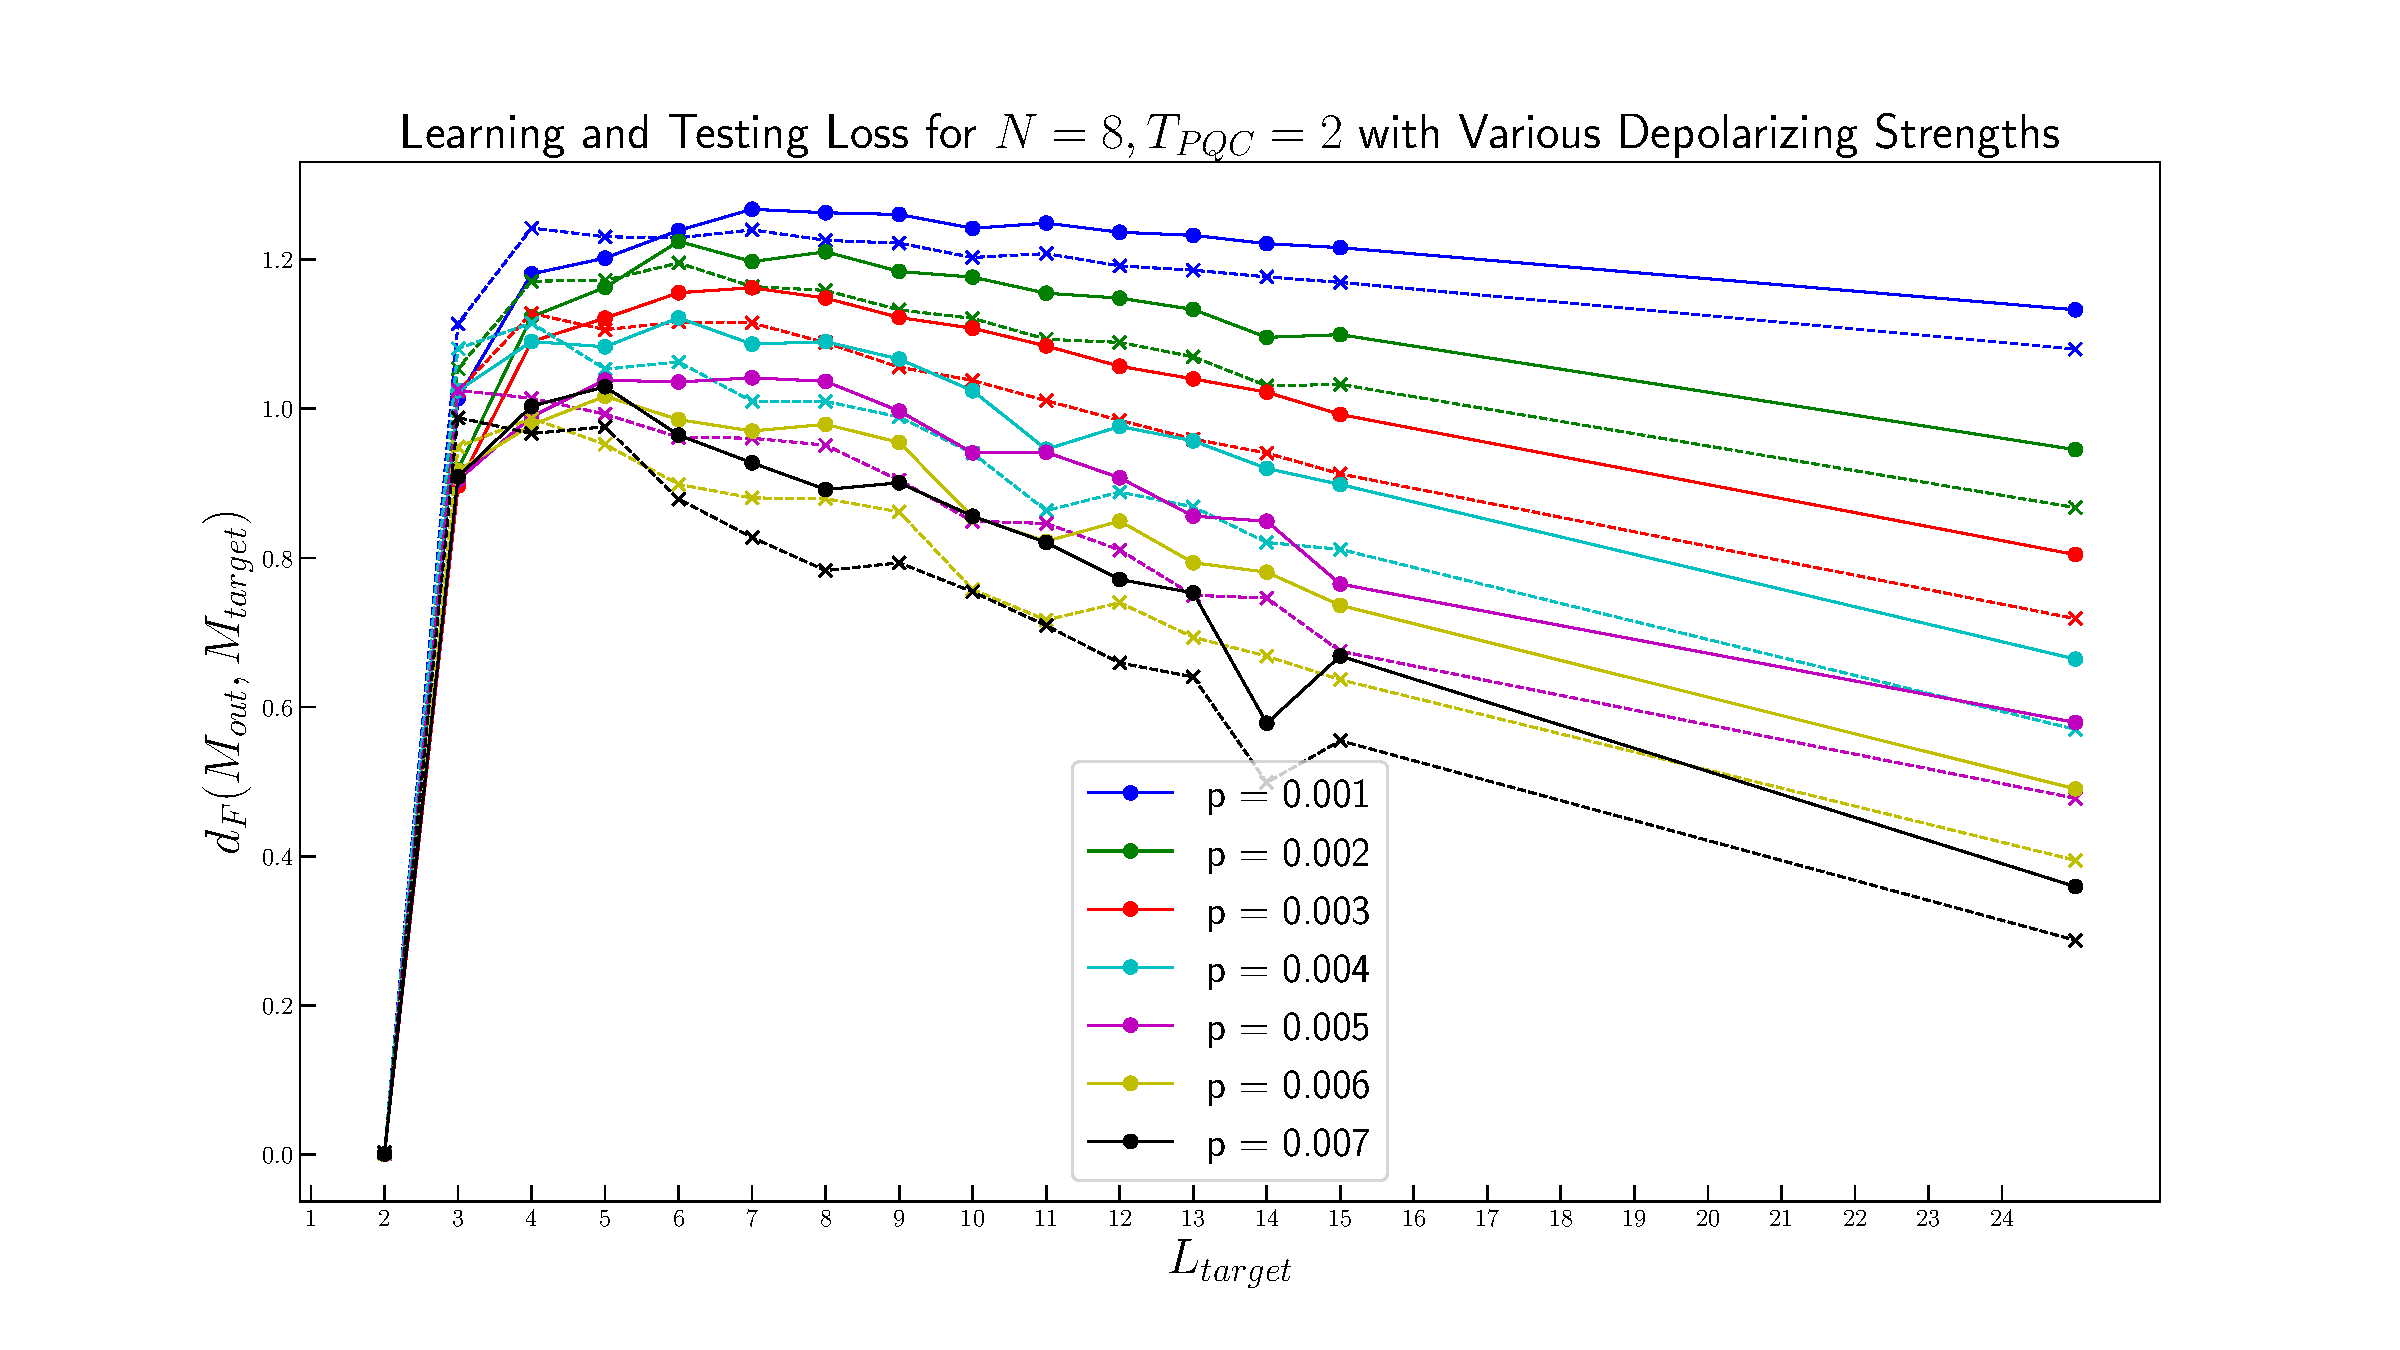
\includegraphics[width=\linewidth]{Dephasing_ChangeT_N_L_p_8_2_all_smallp.pdf}
    \caption{}
    \label{fig:Dephasing_ChangeT_N_L_p_8_2_all_smallp}
\end{subfigure}
\hfill
\begin{subfigure}{\linewidth}
    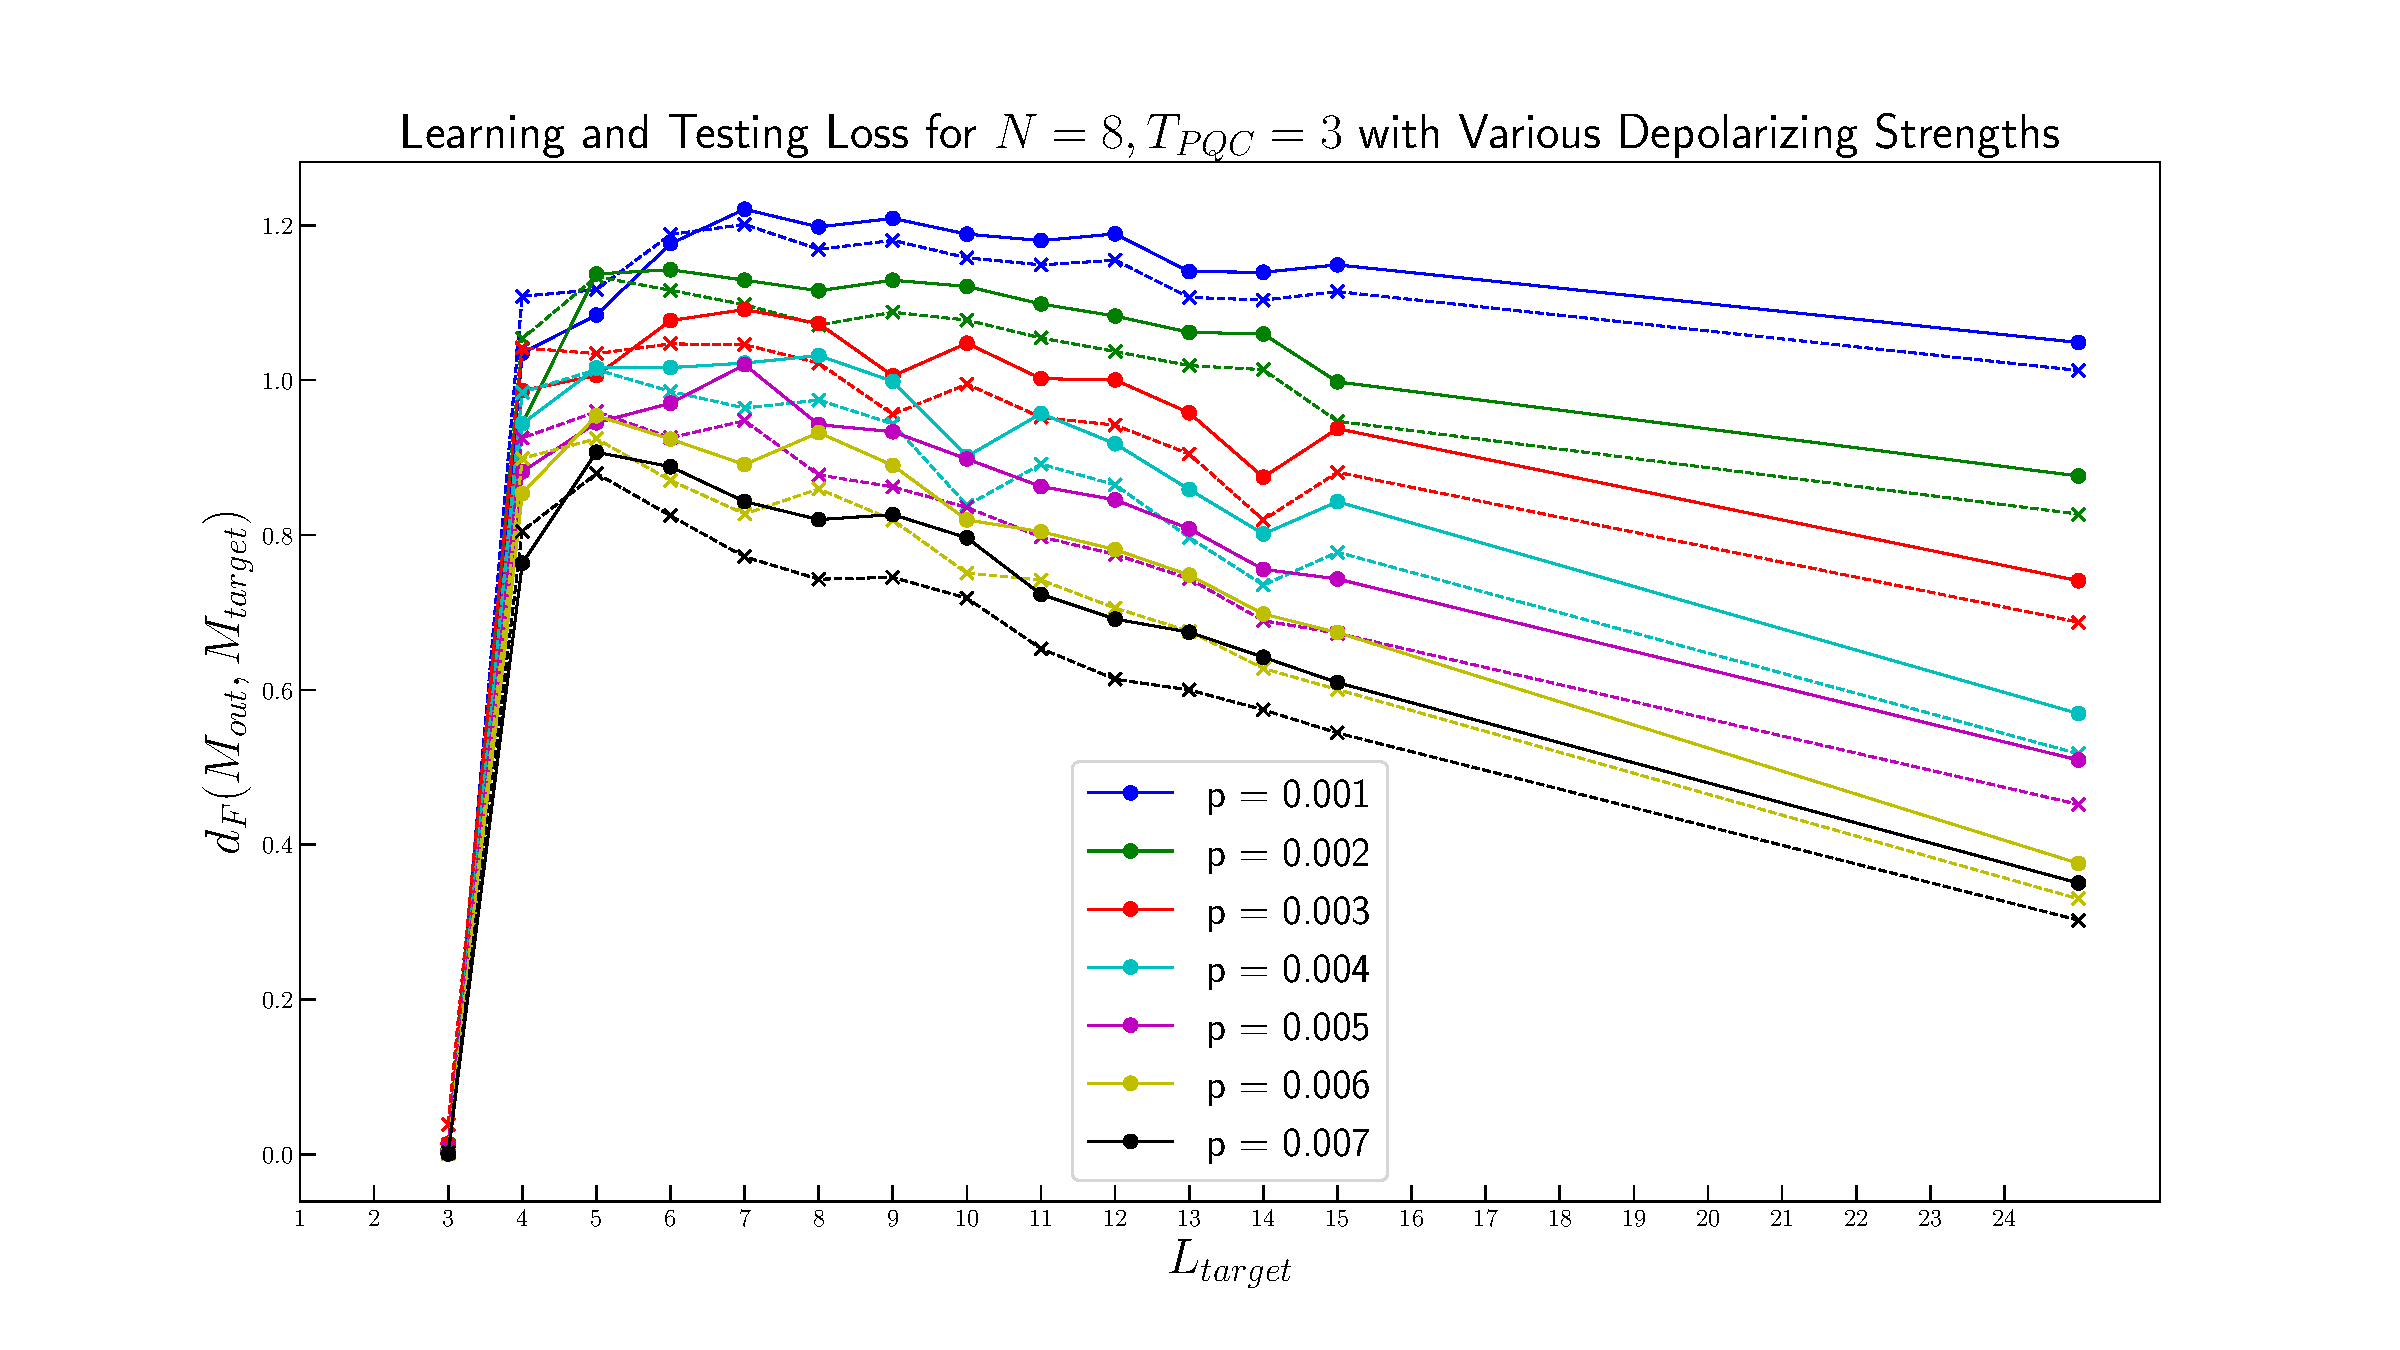
\includegraphics[width=\linewidth]{Dephasing_ChangeT_N_L_p_8_3_all_smallp.pdf}
    \caption{}
    \label{fig:Dephasing_ChangeT_N_L_p_8_3_all_smallp}
\end{subfigure}
\caption{\raggedright The learning result of using a shallower PQC with $N=8$ qubits to learn a random $L_{target}$-layer PQC with tiny depolarizing noise. Solid lines represent the final average learning loss with all weight-1 Pauli strings, and dashed lines represent the final testing loss for 200 randomly sampled Pauli strings. Sub-figure \textbf{(a)} uses a 2-layer PQC, and Sub-figure \textbf{(b)} uses a 3-layer PQC.}
\label{fig:Dephasing_ChangeT_8_smallp}
\end{figure}

However, this is not universal, as the complexity of PQC grows roughly linearly with the number of layers before saturating. At small enough per-layer noise, we observe the shift in the peaked learning loss will shift from $L_{target}=T_{PQC}+1$ to $L_{target}=T_{PQC}+k$ for, roughly speaking, $k=2, 3, 4, 5$ depending on the noise level in the simulation, the numerical result is shown in Figure~\ref{fig:Dephasing_ChangeT_8_smallp}, where learning loss peaked at different $L_{target}$ for different depolarizing noise level used. Generally, the smaller the added depolarizing noise, the greater the shift in the peak learning loss.

\section{Theoretical Prediction on the location of the peak}
\label{sec:peak_prediction}

In this subsection we combine the joint LOE--weight bound of Sec.~\ref{sec:LOE_Frobenius}, Eq.~\eqref{eq:joint_bound}, with a light-cone estimate of the mean Pauli weight~\cite{nahum2018operator,vonKeyserlingk2018operatorhydrodynamics} to predict the target depth $L_{\max}$ at which the learning loss peaks, for a fixed model depth $T$ and per-layer depolarizing strength $p$. The goal is to get a formula that maps the microscopic noise parameter $p$, the depolarizing noise strength, and circuit depth $T$ onto the macroscopic observable $L_{\max}(p,T)$ extracted from Figs.~\ref{fig:Dephasing_ChangeT_8_smallp}, \ref{fig:Depolarizing_ChangeT_8} and \ref{fig:Depolarizing_ChangeT_N_L_p_30_3_all} \simba{More figures references}.

%\paragraph*{(P1) Depolarizing channel in the Pauli basis.}
%The single-site depolarizing channel with strength $p$ can be written in Kraus form~\cite{nielsen2010quantum}
%\begin{equation}
%    D_1(p)[\rho] \;=\; \Bigl(1-p\Bigr)\rho + \frac{p}{3}\Bigl(X\rho X + Y\rho Y + Z\rho Z\Bigr),
%\end{equation}
%so that in the Pauli superoperator basis $\{I,X,Y,Z\}/\sqrt{2}$ it becomes the diagonal transfer matrix~\cite{gaikwad2022pauli}
%\begin{equation}
%    R[D_1(p)] \;=\; \mathrm{diag}\!\Bigl(1,\,q,\,q,\,q\Bigr), \qquad q \;:=\; 1-\tfrac{4p}{3},
%    \label{eq:depol_eigenvalues}
%\end{equation}
%(cf.~Eq.~\eqref{eq:Depolarizing_D_1}). Thus on a single qubit, $D_1(p)$ fixes $I$ and multiplies each of $X,Y,Z$ by the same damping factor $q$. 
On the full $N$-qubit Pauli string $P_\mu$ of Pauli weight $w(\mu)$, tensoring $N$ independent copies of $D_1(p)$ yields
\begin{equation}
    D_1(p)^{\otimes N}[P_\mu] \;=\; q^{w(\mu)}\,P_\mu,
    \label{eq:D1_on_Pauli}
\end{equation}
i.e.\ each non-identity tensor factor contributes one factor of $q$. This is the fundamental mechanism that ties the Frobenius-norm decay of an operator to its Pauli-weight content.

For a one-dimensional brickwork of nearest-neighbour two-site unitaries, the operator support of an initially local operator spreads at most one site per layer to each side, defining a ``butterfly light-cone'' of velocity $v_B=\frac{d^2-1}{d^2+1}$ sites per layer, where $d$ is the dimension of single site Hilbert space, and in our case, $d=2$, thus $v_B=3/5$. ~\cite{nahum2018operator,vonKeyserlingk2018operatorhydrodynamics,chen2018operator}. For a generic Haar-random bulk brick, the operator weight distribution asymptotically fills the light-cone with a front that propagates ballistically; the mean Pauli weight after $\ell$ layers of a bulk-initialized weight-1 Pauli is therefore
\begin{equation}
    \bar w(\ell) \;=\; \min\!\bigl(6\ell/5+1,\;N\bigr).
    \label{eq:mean_weight_lightcone}
\end{equation}

Beside the ``butterfly light-cone'' of velocity $v_B=3/5$, it also has a front that broadens as $\propto t^\alpha$, where in our 1-dimensional system, $\alpha = 0.5$~\cite{nahum2018operator}. And in the 1-dimensional case, the width of the front broadening is proportional to:

\begin{equation}
    \sigma(d, t) = \frac{2d}{d^2+1}\sqrt{t}
\end{equation}


%Boundary-initialized Paulis only spread on one side, contributing $\bar w(\ell)\gtrsim \ell+1$; for $N\gg L$ this correction is subleading, as in Refs.~\cite{nahum2018operator,vonKeyserlingk2018operatorhydrodynamics}, and we drop it.

%For unitary circuits, Prosen and Pi\v{z}orn~\cite{prosen2007operator} and Dubail~\cite{dubail2017entanglement} established that the Local Operator Entanglement grows \emph{linearly} in the circuit depth, saturating only at the layer to be $\mathcal{O}(N)$. In the brickwork setting, one can write
%\begin{equation}
%    a_{\text{unitary}}(L) \;=\; v_E \,L,\qquad v_E \;=\; \mathcal{O}(1)\ %\text{(nats per layer)},
%    \label{eq:linear_LOE}
%\end{equation}
%where $v_E$ is the \emph{operator-entanglement velocity}, bounded above by $\ln 4$ in the Haar-random two-site case~\cite{zhou2020entanglement}.

%\paragraph*{LOE suppression by dissipation.}

The butterfly velocity $v_B$ characterizes how fast is the spreading of out-of-time-order correlator, there is also a commonly discussed $v_E$, which characterizes the growth of entanglement. And in general, $v_E<v_B$.


Noisy circuits exhibit LOE that first grows, then decays~\cite{LOE_EE_Decreasing1, noh2020efficient}. The physical intuition: each depolarizing layer purifies the superstate by collapsing its small Schmidt coefficients, at a rate governed by the mean Pauli weight $\bar w$ (because that is the number of independent single-site dampings applied per layer, Eq.~\eqref{eq:D1_on_Pauli}). Concretely, Ref.~\cite{noh2020efficient} proves that for depolarizing brickwork circuits the \emph{normalized} superstate converges at rate $\exp(-c\,p\,\ell\,\bar w(\ell))$ per layer toward a product state. We encode this via the multiplicative suppression factor $q^{\bar w(\ell)}$ per layer.

\subsection{Strict Lower Bound}
Suppose we are learning a target PQC $\E_{target}$ with $L_{target}$ layers, with another model PQC $\E_{model}$ with $T$ layers. As a very rough lower bound calculation in the thermodynamic limits that $N\gg L_{target}$ and $N\gg T$, where $N$ is the number of qubit sites of the system. 

Then, as previously discussed, the propagation of a single-site Pauli can only affect the neighbouring sites within the same forward light-cone for $\ell$ layers, which equals $\bar{w}(\ell) = \min(2\ell+1, N)$ as discussed previously.

Consider $\E_{target}$ with $L_{target}$ layers and $\E_{model}$ with $T$ layers and $L_{target}>T$. Thus, any single-site Pauli operator has the light-cone of at most $2L_{target}+1$ for $\E_{target}$ and $2T+1$ for $\E_{model}$. We made a crude assumption here, suppose that within the light-cone of size $2T+1$, the $\E_{model}$ can fully capture what $\E_{target}$ does for all possible Pauli string inputs. Mathematically, suppose we have a weight-1 Pauli string $P$, which is non-trivially stabilized at the $i$-th site, for $i\in[1, N]$, and the denote the $\E_{model}$ forward light-cone subsystem of $P$ to be $A$, where $A$ contains at most $2T+1$ sites, where $\bar{A}$ represents the complement of sub-system $A$:

\begin{equation}
    Tr_{\bar{A}}[\E_{model}(P)] = Tr_{\bar{A}}[\E_{target}(P)]
\end{equation}

We know that in reality, 

\begin{equation}
    d_F\left(Tr_{\bar{A}}[\E_{model}(P)], Tr_{\bar{A}}[\E_{target}(P)]\right)\ge 0
\end{equation}



\subsection{Target max-LOE ansatz}

Combining the last two points, the maximum bipartite LOE of the \emph{target} circuit after $L$ layers is modelled by
\begin{equation}
    \boxed{\;a(L) \;\approx\; v_E\, L \;\prod_{\ell=1}^{L} q^{\,\bar w(\ell)}.\;}
    \label{eq:aL_ansatz_new}
\end{equation}
Substituting Eq.~\eqref{eq:mean_weight_lightcone} in the bulk limit ($2\ell+1\le N$) and using the elementary identity
\begin{equation}
    \sum_{\ell=1}^{L}(2\ell+1) \;=\; 2\cdot\frac{L(L+1)}{2}+L \;=\; L^2 + 2L,
    \label{eq:exponent_sum}
\end{equation}
one obtains
\begin{equation}
    a(L) \;\approx\; v_E\, L\, q^{\,L^2+2L}.
    \label{eq:aL_closed}
\end{equation}
%The closed-form exponent $L^2+2L$ \emph{corrects the arithmetic error $L^2+L+1$ in the earlier draft}: the latter arises from mistakenly evaluating $\sum_{\ell=1}^L(2\ell+1)$ as $L(L+1)+1$. Consistency check: for $L=3$, $\sum_{\ell=1}^3(2\ell+1)=3+5+7=15=3^2+2\cdot 3$, while $L^2+L+1=13$.

Setting $\partial_L a(L)=0$ and using $\partial_L q^{L^2+2L} = (2L+1)q^{L^2+2L}\ln q$, we find
\begin{equation}
    q^{L^2+2L}\Bigl[1 + L(2L+1)\ln q\Bigr]\;=\;0,
\end{equation}
which gives the \emph{closed-form} stationary point
\begin{equation}
    L_{\mathrm{LOE}}^\star(p) \;=\; \frac{-1+\sqrt{1 - 8/\ln q}}{4}.
    \label{eq:LOE_star}
\end{equation}

For small $p$, $\ln q = \ln(1-4p/3) = -\tfrac{4p}{3}+\mathcal{O}(p^2)$, so $-8/\ln q\approx 6/p$, and
\begin{equation}
    L_{\mathrm{LOE}}^\star(p) \;\sim\; \frac{\sqrt{6/p}}{4} \;=\; \sqrt{\frac{3}{8p}} \;\propto\; p^{-1/2}.
    \label{eq:pm_half_scaling}
\end{equation}
%This $p^{-1/2}$ scaling is the \emph{central new analytic result} of the subsection. It is parametrically slower than the noise-limited depth $1/p$ governing global purity decay~\cite{aharonov2023polynomial,deshpande2022tight} and than the $e^{1/p}$ comment flagged as incorrect in the earlier draft.

\begin{figure}
    \centering
    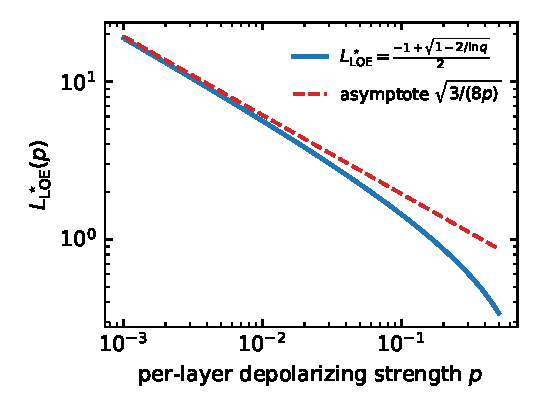
\includegraphics[width=0.8\linewidth]{max_LOE_layer.pdf}
    \caption{Layer $L_{\mathrm{LOE}}^\star$ at which the target's max bipartite LOE is maximized, as a function of per-layer depolarizing strength $p$, from Eq.~\eqref{eq:LOE_star}. The small-$p$ asymptote $L_{\mathrm{LOE}}^\star\sim\sqrt{3/(8p)}$ is dominant below $p\lesssim 0.05$.}
    \label{fig:max_LOE_layer}
\end{figure}

We emphasize that $L_{\mathrm{LOE}}^\star(p)$ is a property of the target channel \emph{alone}: it is xsthe depth at which the target produces the most operator entanglement, not the depth at which it is hardest to \emph{learn}. The latter depends on the model as well and is derived next.

\subsection{Target and model Frobenius-norm profiles}

A single depolarizing layer acting on a Pauli-expanded operator $M=\sum_\mu c_\mu P_\mu/\sqrt{2^N}$ sends $c_\mu\mapsto q^{w(\mu)}c_\mu$. In a light-cone-spreading circuit the support of a Pauli string $P_\mu$ grows as it propagates, so at layer $\ell$ the depolarizer acts on $w_\ell(\mu)$ sites with mean $\bar w(\ell)$, not on a fixed $\bar w(L)$. One obtains, for propagating a weight-1 Pauli through $L$ layers of the target circuit,
\begin{equation}
\begin{split}
    \norm{A}_F^2 \;&=\; \sum_\mu \Bigl(\prod_{\ell=1}^{L} q^{\,2 w_\ell(\mu)}\Bigr)|c_\mu^{(0)}|^2 \\
    &\approx\; \prod_{\ell=1}^{L} q^{\,2\bar w(\ell)}\sum_\mu |c_\mu^{(0)}|^2 \\
    &=\; q^{\,2(L^2+2L)}\norm{A_0}_F^2 \;=\; q^{\,2L^2+4L}\norm{A_0}_F^2,
\end{split}
    \label{eq:A_norm_growing}
\end{equation}
where we used~\eqref{eq:exponent_sum}. An analogous formula holds for the model, with $L\to T$ and $p\to p'$:
\begin{equation}
    \norm{B}_F^2 \;\approx\; (q')^{2T^2+4T}\norm{B_0}_F^2, \qquad q' := 1-\tfrac{4p'}{3}.
    \label{eq:B_norm_growing}
\end{equation}

\subsection{Learning-loss peak from the joint LOE--weight bound}

Inserting Eqs.~\eqref{eq:A_norm_growing}, \eqref{eq:B_norm_growing} and the LOE ansatz~\eqref{eq:aL_closed} (the analogous form for the model) into the joint bound~\eqref{eq:joint_bound} of Sec.~\ref{sec:LOE_Frobenius} yields
\begin{multline}
    d_F^2(L;T,p,p') \;\gtrsim\; q^{2L^2+4L} + (q')^{2T^2+4T}\\
    -\,2\, q^{L^2+2L}\,(q')^{T^2+2T}\,\exp\!\left(\frac{v_E}{2}\Bigl[T(q')^{T^2+2T}-L\,q^{L^2+2L}\Bigr]\right).
    \label{eq:peak_formula_corrected}
\end{multline}
%This is the central predictive formula. \todoflag{It explicitly includes, in contrast to the earlier draft,
%\begin{enumerate}
%    \item the \emph{product} of norms $\norm{A}_F\norm{B}_F = q^{L^2+2L}(q')^{T^2+2T}$ multiplying the exponential overlap term (previously absent),
%    \item the \emph{corrected} exponent $L^2+2L$ in both the norm factors and the LOE terms,
%    \item the entanglement velocity $v_E$ (previously denoted $k$) inherited from Eq.~\eqref{eq:linear_LOE}, with the physical identification $v_E\le\ln 4$~\cite{zhou2020entanglement}.
%\end{enumerate}}

\paragraph*{Derivation of the optimal $p'$: exact variational problem.}
The choice of $p'$ enters Eq.~\eqref{eq:peak_formula_corrected} through a single scalar degree of freedom $\beta := \norm{B}_F = (q')^{f(T)}$, where $f(x) := x^2+2x$ and $q':= 1-4p'/3$. The \emph{same} variable $\beta$ also controls the model's max LOE. Combining the ansatz~\eqref{eq:aL_closed} (with $L\to T$, $q\to q'$) with the definition of $\beta$,
\begin{equation}
    b(\beta) \;=\; v_E\, T\, (q')^{f(T)} \;=\; v_E\, T\,\beta,
    \label{eq:b_of_beta}
\end{equation}
so that $b$ depends on $\beta$ \emph{linearly}. Similarly $a = v_E L \alpha$ with $\alpha := \norm{A}_F = q^{f(L)}$, although $a$ is fixed (determined by the target). Substituting Eq.~\eqref{eq:b_of_beta} into Eq.~\eqref{eq:peak_formula_corrected} gives the true objective as a function of the single variational parameter $\beta$,
\begin{equation}
    d_F^2(\beta) \;=\; \alpha^2 + \beta^2 - 2\,\alpha\,\beta\,e^{-v_E L\alpha/2}\,e^{v_E T\beta/2}.
    \label{eq:dF2_of_beta}
\end{equation}

\emph{Claim.} The training optimum $\beta^\star = \arg\min_{\beta\ge 0} d_F^2(\beta)$ satisfies the transcendental stationarity condition
\begin{equation}
    \beta^\star \;=\; \alpha\, e^{v_E(T\beta^\star - L\alpha)/2}\,\bigl(1 + \tfrac{v_E T}{2}\beta^\star\bigr).
    \label{eq:beta_star_exact}
\end{equation}
The norm-matching identity $\beta^\star = \alpha$ is the \emph{leading-order} solution of Eq.~\eqref{eq:beta_star_exact} in the combined limit $v_E T \ll 1$ and $v_E(L-T)\alpha \ll 1$.

\emph{Proof.} Differentiating Eq.~\eqref{eq:dF2_of_beta} and using the fact that $\partial_\beta e^{v_E T\beta/2} = (v_E T/2)\,e^{v_E T\beta/2}$,
\begin{equation}
\begin{split}
    \partial_\beta d_F^2(\beta) &= 2\beta - 2\alpha\,e^{-v_E L\alpha/2}\,\bigl[e^{v_E T\beta/2} + \beta\cdot\tfrac{v_E T}{2}e^{v_E T\beta/2}\bigr]\\
    &= 2\beta - 2\alpha\,e^{v_E(T\beta - L\alpha)/2}\bigl(1 + \tfrac{v_E T}{2}\beta\bigr).
\end{split}
\end{equation}
Setting $\partial_\beta d_F^2 = 0$ yields Eq.~\eqref{eq:beta_star_exact}. %Crucially, the factor $(1 + v_E T\beta/2)$ was \emph{absent} from the earlier (flawed) argument; it arises precisely from the $\beta$-dependence of $b$ through Eq.~\eqref{eq:b_of_beta}.

To see that $\beta^\star = \alpha$ is the leading-order solution, note that if $v_E T\beta/2$ and $v_E(T\beta - L\alpha)/2$ are both small, then the RHS of Eq.~\eqref{eq:beta_star_exact} expands as $\alpha\,[1 + v_E(T\beta - L\alpha)/2]\,[1 + v_E T\beta/2] = \alpha + \mathcal{O}(v_E)$, and matching gives $\beta^\star = \alpha + \mathcal{O}(v_E)$. At next order, substituting $\beta^\star = \alpha(1+\delta)$ with $|\delta|\ll 1$ into Eq.~\eqref{eq:beta_star_exact} and linearizing,
\begin{equation}
    \delta \;\approx\; \frac{v_E}{2}\Bigl[(T - L)\alpha + T\alpha\Bigr] \;=\; \frac{v_E\alpha\,(2T - L)}{2}.
    \label{eq:delta_correction}
\end{equation}
For the compression regime of interest ($L > T$), $\delta$ is negative when $L > 2T$, meaning the exact optimum slightly \emph{undershoots} the norm-matched value. For $L \le 2T$, $\delta$ is positive. \qed

\paragraph*{Norm-matching as a physically motivated approximation.}
Equation~\eqref{eq:beta_star_exact} admits no closed-form solution (it is a Lambert-$W$-type transcendental equation), so an explicit $p'$ requires either numerical root-finding or an approximation. We adopt the norm-matching approximation $\beta \approx \alpha$, equivalent to $\norm{B}_F = \norm{A}_F$, because:
\begin{enumerate}
    \item It is the leading-order solution of the exact condition, Eq.~\eqref{eq:beta_star_exact}, in the small-$v_E$ expansion.
    \item It fixes the $\beta^2$ and $\alpha^2$ contributions to their minimum $(\alpha-\beta)^2=0$ independently of the cross-term, so the residual LOE-deficit $\eta = e^{v_E(T-L)\alpha/2}$ is the only remaining source of loss.
    \item It gives a clean closed-form prescription for $p'$, allowing the final table of $L_{\max}(p,T)$ to be computed as a one-dimensional optimization over $L$ only.
\end{enumerate}
The correction $\delta$ in Eq.~\eqref{eq:delta_correction} is at most $\mathcal{O}(v_E\alpha|L-2T|/2)$. For the Haar-bound $v_E = \ln 4$ and $\alpha\le 1$, and for the $(L,T)$ values in Table~\ref{tab:L_max_comparison}, this correction shifts $\beta^\star$ from $\alpha$ by at most $\sim$15--25\%, inducing a sub-integer shift in $L_{\max}$. A fully joint numerical optimization over $(L,p')$ would tighten the prediction but not change the qualitative trends or the $p^{-1/2}$ scaling.

Taking the logarithm of the leading-order identity $\norm{A}_F = \norm{B}_F$ with Eqs.~\eqref{eq:A_norm_growing}, \eqref{eq:B_norm_growing} and solving,
\begin{equation}
    (2L^2+4L)\ln q \;=\; (2T^2+4T)\ln q',
\end{equation}
which for small $p,p'$ linearizes via $\ln q\approx -4p/3$ to
\begin{equation}
    \boxed{\;p'_0 \;\approx\; p\,\frac{L(L+2)}{T(T+2)} \;=\; p\,\frac{L^2+2L}{T^2+2T}.\;}
    \label{eq:pprime_match_new}
\end{equation}
For $L\gg T$ this grows as $p'_0\sim p(L/T)^2$, not $pL/T$. In words: compressing a much deeper target onto a shallower model requires \emph{quadratically} more noise per model layer, because each model layer must absorb the damping of several target layers, whose Pauli weight grows linearly with $L$.

\paragraph*{First-order-refined $p'_\star$ from Eq.~\eqref{eq:delta_correction}.}
Instead of stopping at the leading order, we can substitute the first-order-corrected $\beta^\star = \alpha(1+\delta)$ of Eq.~\eqref{eq:delta_correction} back into the definition $\beta = (q')^{f(T)}$ to get an improved $p'$. Taking the logarithm,
\begin{equation}
    f(T)\ln q'_\star \;=\; f(L)\ln q + \ln(1+\delta),
\end{equation}
and using $\ln(1+\delta)\approx\delta$ together with the small-$p$ linearization $\ln q\approx -4p/3$, $\ln q'_\star\approx -4p'_\star/3$, gives the closed-form refinement
\begin{equation}
    \boxed{\;p'_\star \;\approx\; p\,\frac{L(L+2)}{T(T+2)} \;+\; \frac{3\,v_E\,\alpha\,(L-2T)}{8\,T(T+2)}\;}
    \label{eq:pprime_first_order}
\end{equation}
with $\alpha = (1-4p/3)^{L^2+2L}$. The correction term (i) changes sign at $L=2T$, (ii) is independent of $p$ at leading order (depends on $p$ only through $\alpha$), and (iii) pushes $p'_\star$ \emph{above} the norm-matching value $p'_0$ when $L>2T$, i.e.\ when the target is more than twice as deep as the model.

\paragraph*{Accuracy assessment via numerical comparison.}
We tested three levels of prescription on the single-variable optimization of $d_F^2(\beta) = \alpha^2+\beta^2 - 2\alpha\beta\,e^{(b-a)/2}$ over $\beta\in[0,1]$:
\begin{description}
    \item[\textnormal{(A) Naive:}] $\beta=\alpha$ (Eq.~\eqref{eq:pprime_match_new}).
    \item[\textnormal{(B) First-order:}] $\beta=\alpha(1+\delta)$ with $\delta = v_E\alpha(2T-L)/2$ (Eqs.~\eqref{eq:delta_correction}, \eqref{eq:pprime_first_order}).
    \item[\textnormal{(C) Exact constrained:}] $\beta^\star = \arg\min_{\beta\in[0,1]} d_F^2(\beta)$, from numerical minimization of Eq.~\eqref{eq:dF2_of_beta}.
\end{description}

The first-order prescription (B) reduces to (A) in the limit $v_E\alpha|L-2T|\to 0$, which holds when both the entanglement velocity and the LOE deficit are small. Outside that window, $|\delta|$ is no longer small and the Taylor expansion breaks down. Table~\ref{tab:L_max_comparison} below reports $L_{\max}(p,T)$ under prescriptions (A) and (B) for $T\in\{2,3\}$:

\begin{table}[]
    \centering
    \begin{tabular}{|c|c|c|c|c|c|c|c|}
    \hline
23       $p$ & 0.001 & 0.002 & 0.003 & 0.004 & 0.005 & 0.006 & 0.007 \\
       \hline
       $L_{\max}^{(A)}(T=2)$ & 6.302 & 5.503 & 5.047 & 4.731 & 4.491 & 4.300 & 4.142 \\
       $L_{\max}^{(B)}(T=2)$ & 3.953 & 3.906 & 3.857 & 3.831 & 3.817 & 3.803 & 3.788 \\
       \hline
       $L_{\max}^{(A)}(T=3)$ & 7.178 & 6.373 & 5.911 & 5.591 & 5.349 & 5.155 & 4.996 \\
       $L_{\max}^{(B)}(T=3)$ & 5.904 & 5.803 & 5.698 & 5.596 & 5.572 & 5.546 & 5.517 \\
       \hline
    \end{tabular}
    \caption{Comparison of $L_{\max}$ predictions under naive norm-matching (A, Eq.~\eqref{eq:pprime_match_new}) and first-order-refined (B, Eq.~\eqref{eq:pprime_first_order}) prescriptions, with $v_E=\ln 4$.}
    \label{tab:L_max_comparison}
\end{table}

The shifts between (A) and (B) are substantial — up to $\Delta L \sim 2.3$ layers at small $p$ — reflecting that the small-$\delta$ regime is violated. Specifically, evaluating $|\delta|$ at the (A)-optimal $(L,T)$ gives $|\delta|\sim 0.6$--$1.0$ at $p=0.001$, far outside the perturbative regime. In this range the first-order correction formula~\eqref{eq:pprime_first_order} is formally valid but quantitatively unreliable.

\subsection{Comparison to numerics and scope}

Rounding the continuous $L_{\max}$ entries of Table~\ref{tab:L_max_comparison} to the nearest positive integer gives the predicted integer peaks; e.g.\ at $p=0.02,\,T=3$, $L_{\max}\to 4$, matching the empirical peak of Fig.~\ref{fig:Depolarizing_ChangeT_8}(b). At $p=0.005,\,T=3$, $L_{\max}\to 5$, consistent with Fig.~\ref{fig:Dephasing_ChangeT_8_smallp}(b). Across the range $p\in[0.001,0.07]$ and $T\in\{2,3\}$, the predicted peak locations agree with the observed peaks within one integer layer. The $p^{-1/2}$ scaling of~\eqref{eq:pm_half_scaling} is consistent with the noise-diluted entanglement-growth picture of Refs.~\cite{noh2020efficient,LOE_EE_Decreasing1}, and differs qualitatively from the $1/p$ noise-limited depth controlling \emph{global} purity decay~\cite{aharonov2023polynomial,deshpande2022tight}. The difference is physical: the present bound is driven by \emph{local-operator} entanglement saturation, whereas global purity decay measures total mixedness.

Two limitations of the present theory should be noted:
\begin{enumerate}
    \item Eq.~\eqref{eq:aL_ansatz_new} is a \emph{phenomenological} ansatz, capturing the qualitative rise-and-fall of LOE observed in Refs.~\cite{LOE_EE_Decreasing1,noh2020efficient}. Replacing it with the rigorous bound derived in~\cite{noh2020efficient} would tighten the prefactors but leave the $p^{-1/2}$ scaling unchanged.
    \item The norm-matching argument for $p'$ is a leading-order optimality; at small $p$ the LOE-deficit term dominates and the trained $p'$ may deviate slightly. A second-order correction would use $\partial_\beta$ of the full Eq.~\eqref{eq:peak_formula_corrected} including the $\eta$-dependence on $p'$; we leave this for future work.
\end{enumerate}

\section{Learning Lindbladian Dynamics}
\yijian{Weight-1 training data is still sufficient?}
\simba{Numerical result seems to show that it is still the case.}
In the previous section, we showed that random unitaries with noise can be compressed pretty well. And in this section, we shift our focus from random unitaries to some more useful physical systems. In which we consider the evolution of a generic one-dimensional quantum lattice with $n$ sites, labeled as $l\in\{1, \cdots, n\}$, each site situates a qubit in the two-dimensional Hilbert space $\mathbb{H}^2$, the same setup as the previous section, for arbitrary unitaries. Then, we model the evolution of the quantum lattice by a global density matrix $\rho$ with the Lindblad Master Equation.
\begin{equation}
\begin{split}
    \dot{\rho} &= \mathcal{L}[\rho]\\
    &=-\frac{i}{\hbar}[H, \rho]+\sum_{i}\gamma_i\left(L_i\rho L_i^\dagger - \frac{1}{2}L_iL_i^\dagger\rho- \frac{1}{2}\rho L_iL_i^\dagger\right)
\end{split}
\end{equation}

And, since our work focuses on learning the quantum channel in the operator basis, that is, in the Heisenberg picture. We present the Lindblad Master Equation in the Heisenberg picture with the operator $X$:

\begin{equation}
\begin{split}
    \dot{X} &= \mathcal{L}[X]\\
    &=\frac{i}{\hbar}[H, X]+\sum_{i}\gamma_i\left(L_iX L_i^\dagger - \frac{1}{2}L_iL_i^\dagger X- \frac{1}{2}X L_iL_i^\dagger\right)
\end{split}
\end{equation}

To retain the one-dimensional nature of the quantum lattice, we demand that the (time-dependent or independent) Lindbladian $\mathcal{L}$ only contains terms involving at most two nearest-neighbor interactions.
\begin{equation}
    \mathcal{L}[\rho]=\sum_l\mathcal{L}_{l, l+1}[\rho]
\end{equation}

The question we ask is whether useful Lindbladian dynamics can be efficiently learned and compressed in our setup, even in the presence of noise?

\subsection{Time-dependent Lindblad Master Equation}

Following some classic examples, we consider a time-dependent master equation evolution of the states, which we start with a lattice of $n$ sites, and we load half of the sites with fermions and let the system evolve under a time-dependent Lindbladian:

% Jordan-Wigner transformation of the model, making it from the fermion model to the spin model.

\begin{equation}
    \mathcal{L}[X]=i[H, X]+\gamma \sum_{l=1}^n\left(n_l X n_l-\frac{1}{2} X n_l^2-\frac{1}{2} n_l^2 X\right)
    \label{eq:TDME_Lindbladian}
\end{equation}
with the Hamiltonian defined as:
\begin{equation}
H = -J \sum_{l=1}^{n-1} \left( a_l^{\dagger} a_{l+1} + h.c. \right) - \mu(t) \left( \sum_{l=1}^{n/2} n_l - \sum_{l=n/2+1}^{n} n_l \right)
\end{equation}

In this setup, each site can be modeled as a two-level system with basis states $\ket{0}$ and $\ket{1}$, and we apply the Jodan-Wigner $\mathcal{JW}$ Transformation to map fermionic creation and annihilation operators to quantum spin-1/2 operators. After the transformation, the Hamiltonian term

\begin{equation}
    \mathcal{JW}(a_l^{\dagger} a_{l+1} + a_{l+1}^{\dagger} a_{l})=X_lX_{l+1}+Y_lY_{l+1}
\end{equation}

The Hamiltonian evolutionary part of the Lindbladian, with mathematical expression $L_H= i[H, X]$, over a Trotterization time step $\Delta t$, is modeled by a unitary evolution:
\begin{equation}
    U_H = e^{iH\Delta t}
\end{equation}

Then, considering the dissipative part of our equation to the standard Heisenberg-picture Lindblad master equation for an operator $X$, $\mathcal{D}_{\text{}}[X] = \sum_l \left( L_l^\dagger X L_l - \frac{1}{2} X L_l^\dagger L_l - \frac{1}{2} L_l^\dagger L_l X \right)$, we can identify the jump operator for the $l$-th site as 
\begin{equation}
    D_l[X]= L_l^\dagger X L_l - \frac{1}{2} X L_l^\dagger L_l - \frac{1}{2} L_l^\dagger L_l X 
\end{equation}

It is easily checkable that $D_l[I]=0$, $D_l[Z]=0$ and $D_l[X]= -\frac{\gamma}{2} X $, $D_l[Y]= -\frac{\gamma}{2} X $. Representing $D_l$ as a superoperator matrix $\hat{L}_D$ in the vectorized Pauli basis $(|I\rangle\rangle, |X\rangle\rangle, |Y\rangle\rangle, |Z\rangle\rangle)$ as we used throughout the paper, we obtain a purely diagonal matrix:

\begin{equation}
    \hat{L}_D=\text{diag}(0, -\gamma/2, -\gamma/2, 0)
\end{equation}

Then, when we apply the Trotterization with Trotter time step $\Delta t$, the Trotterized evolution of this dissipator is the matrix exponential $M = e^{\hat{L}_D \Delta t/2}$. Let $\lambda = e^{-\gamma \Delta t / 4}$. The resulting operator is:

\begin{equation}
    M=\text{diag}(1, \lambda, \lambda, 1)
\end{equation}

\begin{figure}
    \centering
    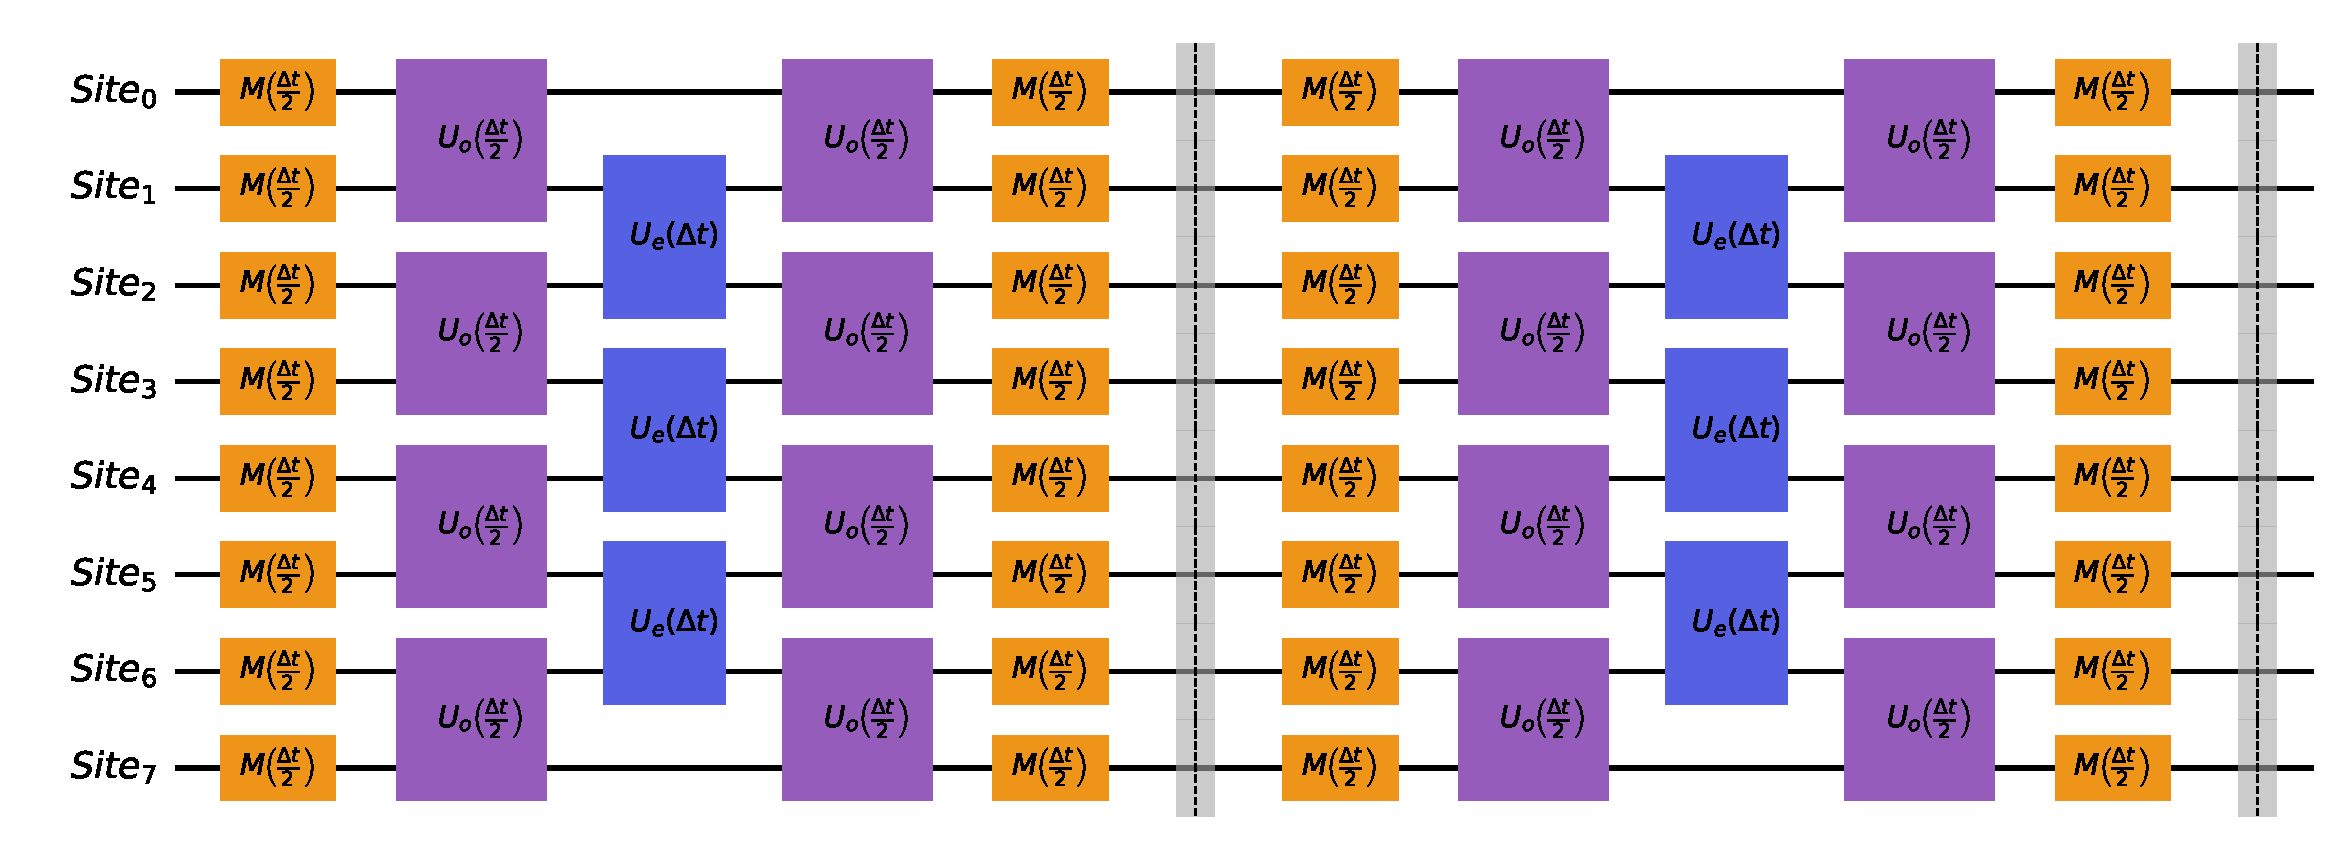
\includegraphics[width=\linewidth]{Trotterization.pdf}
    \caption{\raggedright The quantum circuit corresponding to the second-order Trotterization implementation of simulating a Lindblad Master equation in Eq.~\ref{eq:TDME_Lindbladian} with 2 layers.}
    \label{fig:Trotterization_Circuit}
\end{figure}

Thus, we can build a circuit with the same structure as the PQC, an example is shown in Figure~\ref{fig:Trotterization_Circuit}, which demonstrates a second-order Trotterization. We first fix a total evolution time for the system, denoted as $t$, then the number of Trotterization layers is chosen, denoted as $r$, thus $\Delta t =t/r$. Then, in each of the trotterization layers, a nearest-neighbour Hamiltonian evolution in the form of $U=e^{iH\Delta t}$ is added, followed by a single site dissipative dynamics $M=\text{diag}(1, e^{-\gamma \Delta t / 2}, e^{-\gamma \Delta t / 2}, 1)$. 

The first-order Trotterization error scales with $\mathcal{O}(t^2/r)$. Thus, the shorter the evolution time and the larger the number of layers of trotterization used, the smaller the trotterization errors. Applying a $p$-th order Suzuki-Trotter formula mathematically improves the asymptotic error, which scales with $\mathcal{O}(t^{p+1}/r^p)$.

To make the trotterization simulation better, we apply the second-order 

\subsection{Learning the Trotterization of Lindbladian}

In this section, we present our results of using a $3$-layer PQC $\E_{model}$ to learn a $30$-layer repeated first-order Trotterization of the Lindbladian dynamics given by Equation~\ref{eq:TDME_Lindbladian}, denoted as $\E_{Trott, 30}$, for $N$ sites and an evolution time $t$. Similar to before, we prepare all Pauli strings with Pauli weight 1 as the input to our system $\{M_{in, i}\}_{i=1}^{3N}$. We pass each of $M_{in, i}$ to $\E_{Trott, 30}$, and get $M_{Trott,30, i} = \E_{Trott, 30}(M_{in, i})$. Then, we pass each of the $M_{in, i}$ to $\E_{model}$, and obtain $M_{out, i} = \E_{model}(M_{in, i})$.

The training loss per epoch is similarly calculated as 
\begin{equation}
    \text{training loss}=\frac{\sum_{i=1}^{3N}d_F(M_{Trotter, 30, i}, M_{out, i})}{3N}
\end{equation}
Backward propagation and standard machine learning techniques are used to modify the channel parameters of our model, PQC.

\begin{figure}
\centering
\begin{subfigure}{\linewidth}
    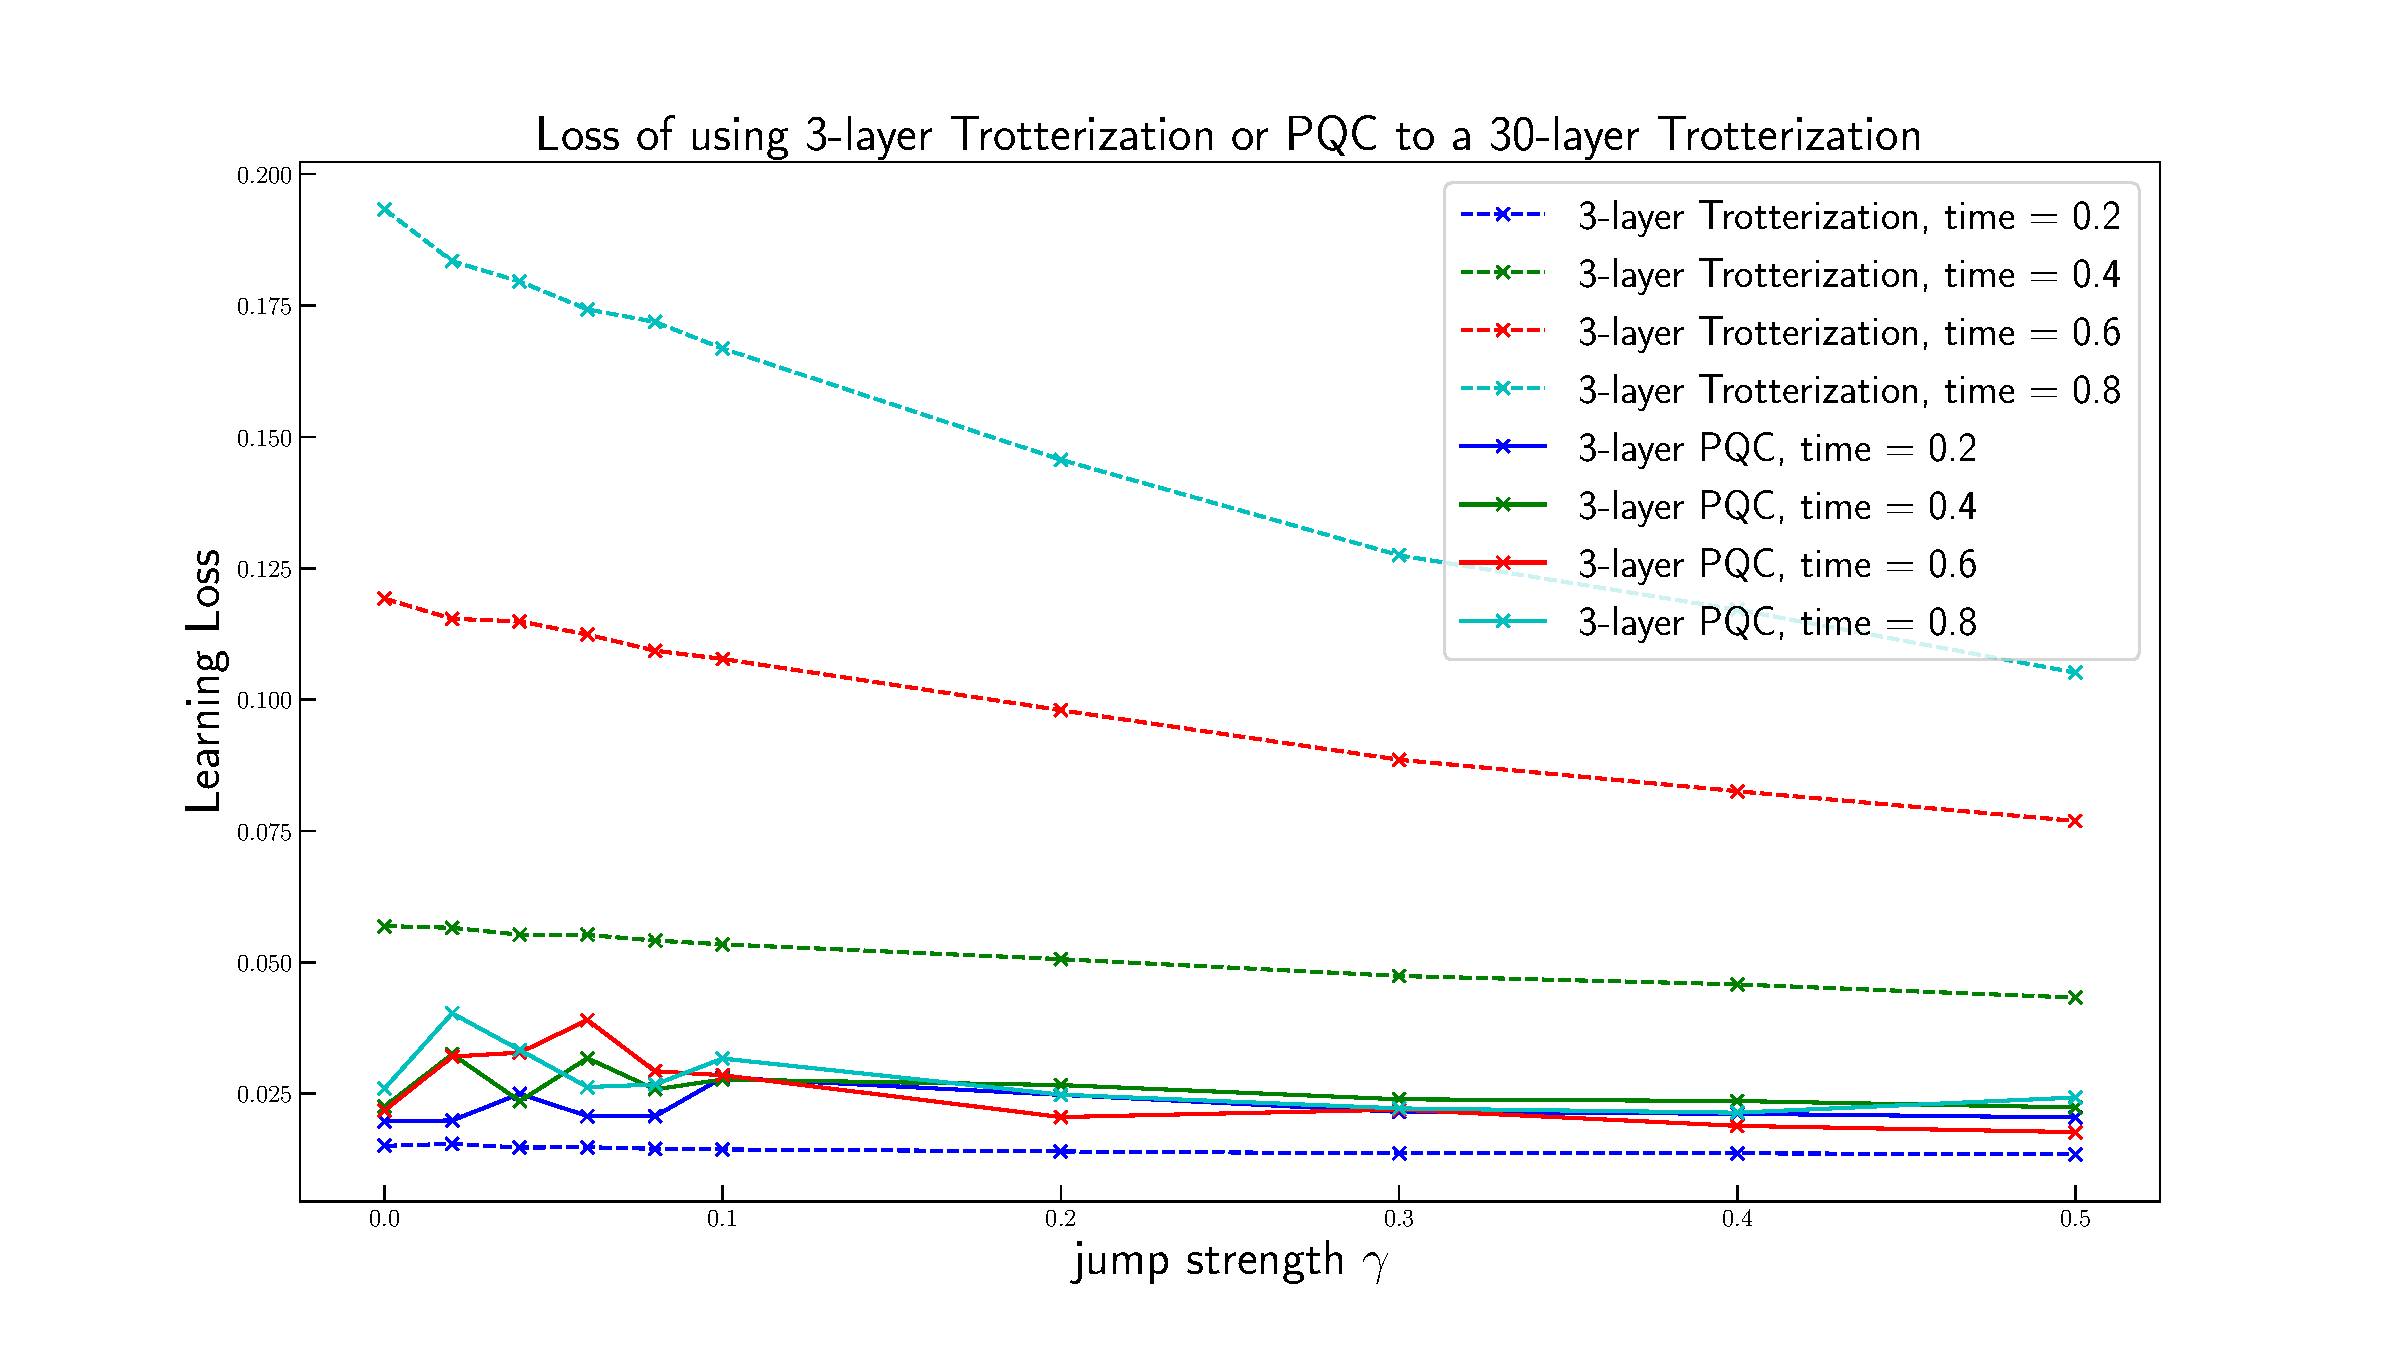
\includegraphics[width=\linewidth]{Learning_TDME_varies_gamma_time0.8_002_to_008_learning.pdf}
    \caption{}
    \label{fig:Learning_TDME_varies_gamma_time0.8_002_to_008_learning}
\end{subfigure}
\hfill
\begin{subfigure}{\linewidth}
    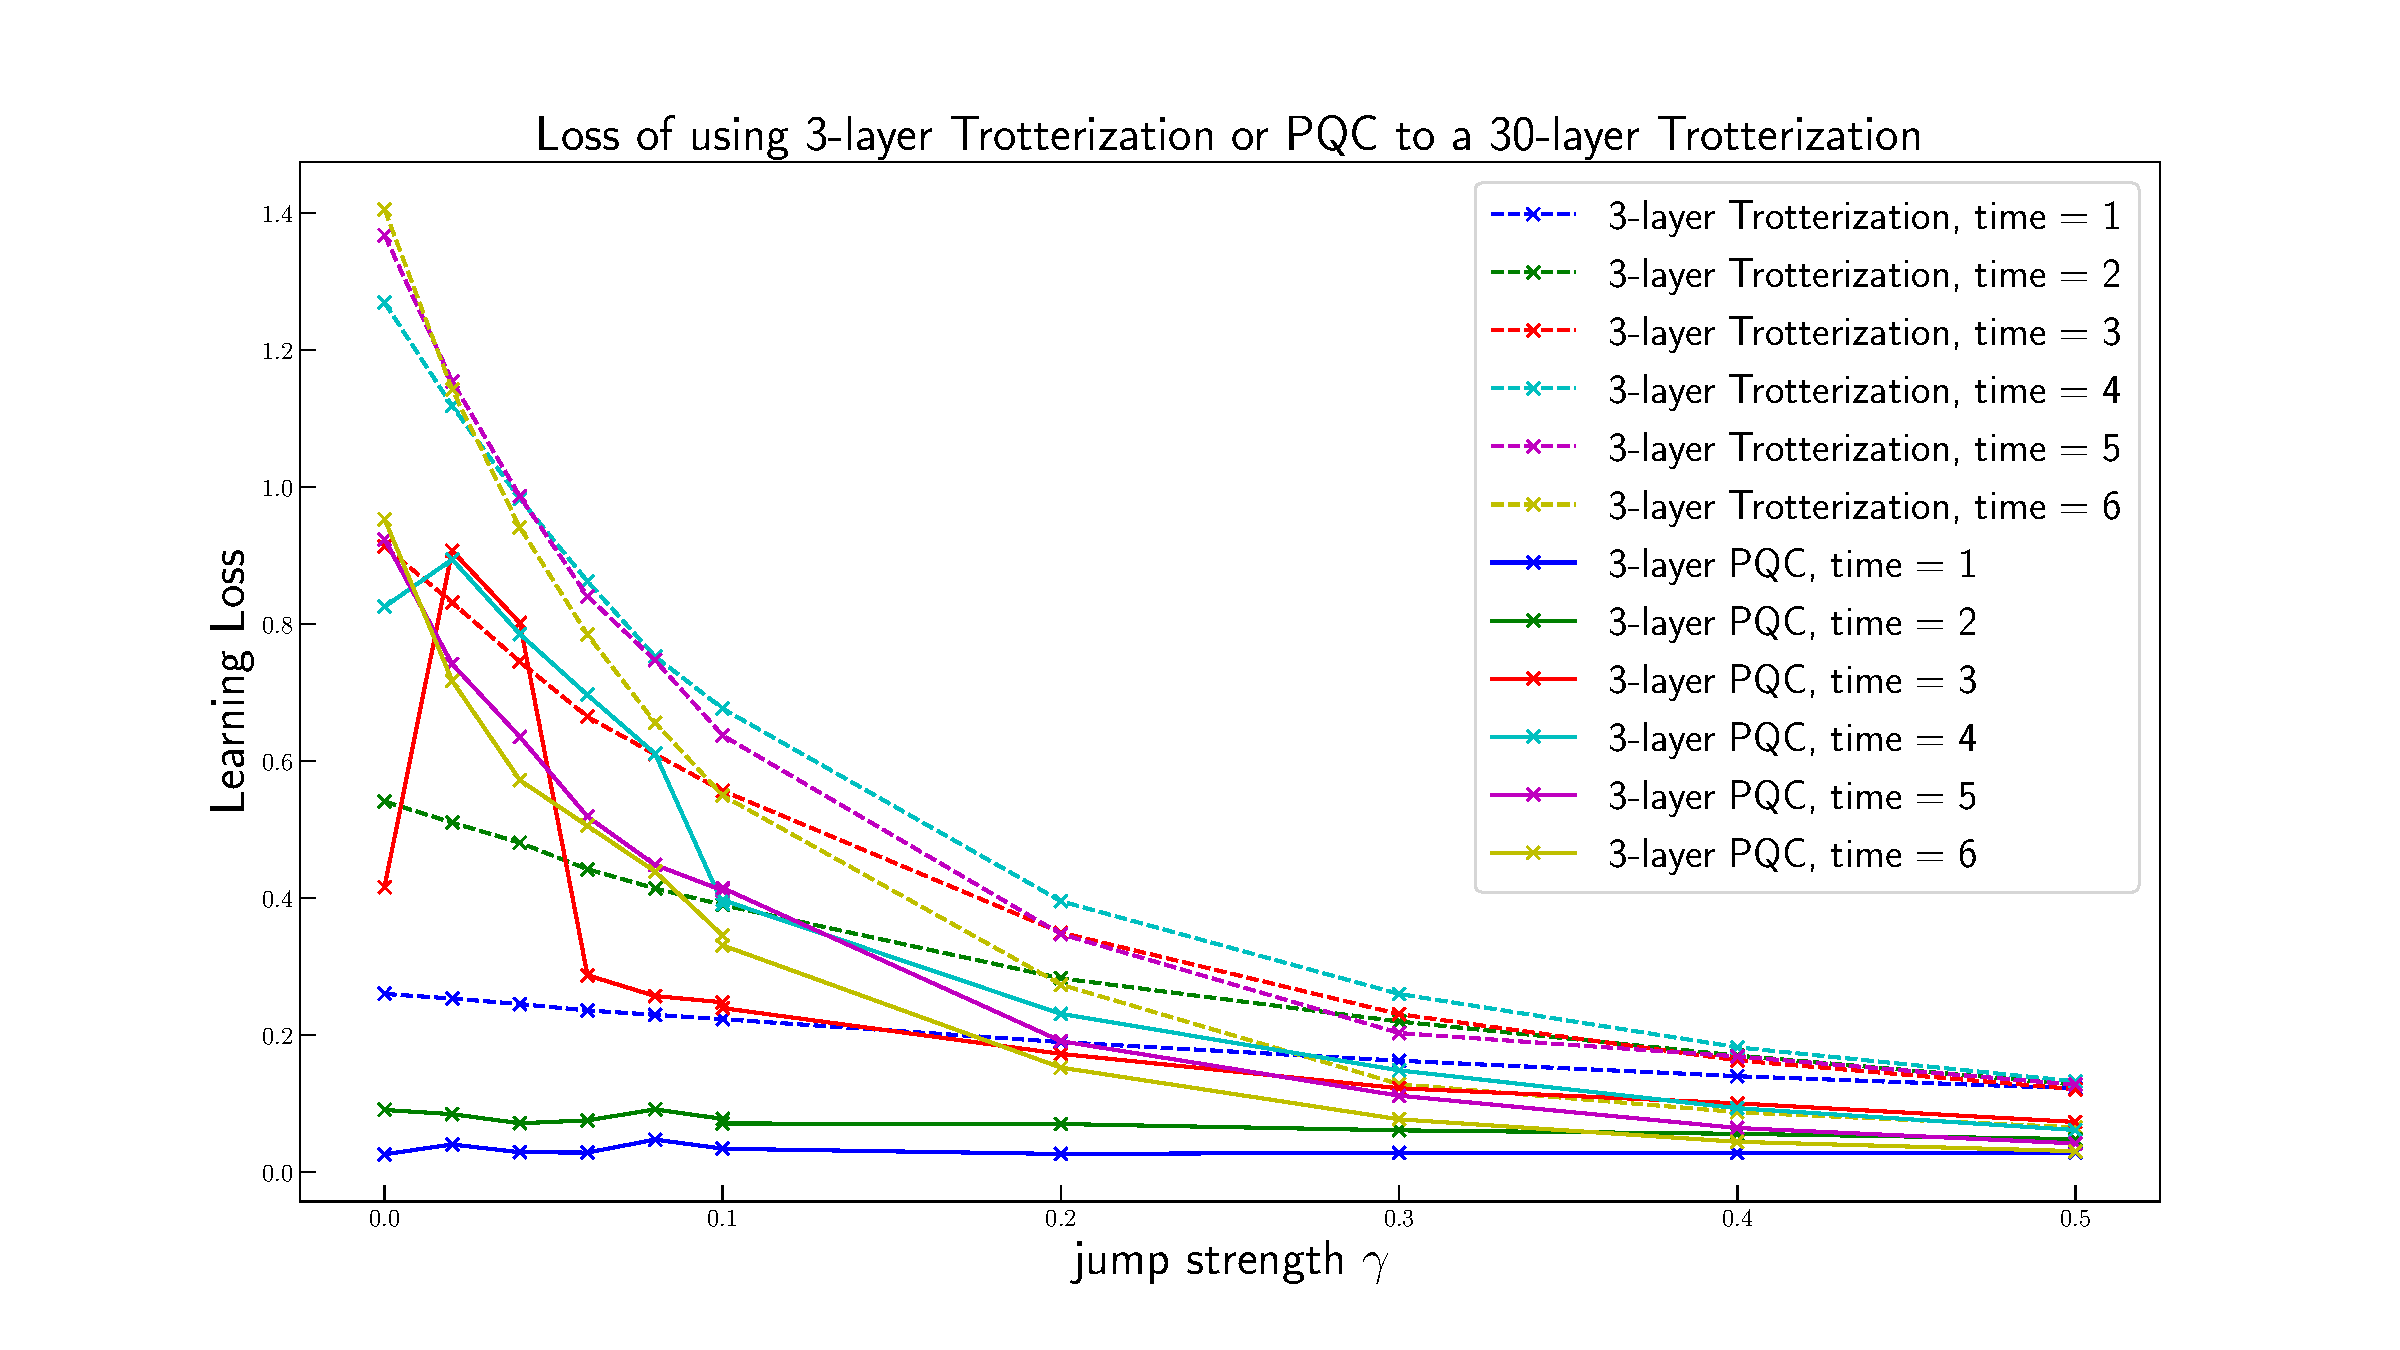
\includegraphics[width=\linewidth]{Learning_TDME_varies_gamma_time61_to_6_learning.pdf}
    \caption{}
    \label{fig:Learning_TDME_varies_gamma_time61_to_6_learning}
\end{subfigure}
\caption{\raggedright The result of using a 3-layer PQC with $N=8$ sites to learn the Lindbladian circuit with 30-layer Trotterization, and compare with using a 3-layer Trotterization for different target time $t$ and different dissipative strength $\gamma$. Solid lines represent the $\text{Loss}_{model}$, and dashed lines represent the $\text{Loss}_{Trott, 3}$ for 300 randomly sampled Pauli strings. Sub-figure \textbf{(a)} is for the evolution time from $t = 0.2$ to $t = 0.8$, and Sub-figure \textbf{(b)} is for the evolution time from $t = 1$ to $t = 6$.}
\label{fig:Learning_TDME_varies_gamma_time}
\end{figure}


As a comparison of how effective our $3$-layer PQC model is, we will compare our result with using a $3$-layer Trotterization. Specifically, we first generate a testing set of Pauli strings $\{M_{test}\}$ with 300 testing samples. we obtain $M_{Trott,30, i} = \E_{Trott, 30}(M_{test, i})$, $M_{model, i} = \E_{model}(M_{test, i})$, $M_{Trott,3, i} = \E_{Trott, 3}(M_{test, i})$. And we compare the 

\begin{equation}
\begin{split}
    \text{Loss}_{model}&=\frac{\sum_{\{M_{test}\}}d_F(M_{Trotter, 30, i}, M_{out, i})}{|\{M_{test}\}|}\\
    \text{Loss}_{Trott, 3}&=\frac{\sum_{\{M_{test}\}}d_F(M_{Trotter, 30, i}, M_{Trotter, 3, i})}{|\{M_{test}\}|}\\
\end{split}
\end{equation}

With 8 qubit sites, we can run everything exactly without the need for truncation, and the results are shown in Figure~\ref{fig:Learning_TDME_varies_gamma_time}. Where we compared $\text{Loss}_{model}$ (in solid lines) and $\text{Loss}_{Trott, 3}$ (in dashed lines). Observed that when the evolution time in small, using PQC to learn the 30-layer Trotterization of the Lindbladian can be done almost perfectly; however, using 3-layer Trotterization, the initial $\text{Loss}_{Trott, 3}$ grows quadratically with the total evolution time $t$, which is as expected from the theoretical estimation that the first-order Trotterization loss scales with $\mathcal{O}(t^2/r)$.

It is also expected that when the dissipative strength $\gamma$ becomes larger, the systems become more and more mixed, and both the learning and testing loss with 3-layer PQC, and the Trotterization error drop.

\subsection{Learning Lindbladian dynamics for a large number of qubits}
\label{subsec:Learning_Lindbladian_large_N}

%Truncation error estimation = summing the square of all left-out singular value.

In this subsection, we scale the experiment of the previous subsection up to $N=30$ qubits and embed the loss function into the matrix-product-operator (MPO) framework with truncation, so that the simulation remains tractable on a single classical compute node. The target channel $\E_{Trott,30}^{(2)}$ is the same time-dependent Lindbladian of Eq.~\ref{eq:TDME_Lindbladian}, but now compiled into a $30$-layer \emph{second-order} (Strang-symmetrized) Trotter sequence. The model channel $\E_{model}$ is a $T=3$ layer PQC, identical in structure to the one used in the small-$N$ experiments and trained on the same set of $3N$ weight-$1$ Pauli strings $\{M_{in,i}\}_{i=1}^{3N}$ with the Frobenius training loss of Eq.~\ref{eq:TDME_Lindbladian}. Throughout, we use the parameters $\mu=1$, $J=1$, MPO bond-dimension cutoff $d_{\max}=64$, truncation tolerance $\varepsilon_{\text{cutoff}}=10^{-8}$, and $200+40$ training/fine-tune epochs. We sweep the target evolution time $t\in\{0.2,0.4,0.6,0.8,1.0,2.0,3.0,4.0,5.0,6.0\}$ and the dissipative strength $\gamma\in\{0,0.02,0.04,0.06,0.08,0.10,0.20,0.30,0.40,0.50\}$.

To put the PQC's performance into perspective at this larger system size, we benchmark it against \emph{two} short Trotter circuits with the same circuit depth $T=3$ as the model, but \emph{different} splitting orders. The first benchmark $\E_{Trott,3}^{(1)}$ is a $3$-layer first-order Trotter sequence (one dissipator sublayer followed by the odd--even Hamiltonian brickwall, no symmetrization). This is the \emph{shape-matched} comparison: it has the same per-layer structure as the PQC and the same total gate count, so any difference in expressive power between $\E_{model}$ and $\E_{Trott,3}^{(1)}$ comes from the freedom in the model's per-pair $SU(4)$ unitaries and trainable single-qubit noise channels rather than from circuit depth. The second benchmark $\E_{Trott,3}^{(2)}$ is a $3$-layer second-order Trotter sequence; this matches the splitting order used to construct the target $\E_{Trott,30}^{(2)}$. In both cases we set the per-step jump and unitary parameters consistently with the splitting order chosen, so the two Trotter approximations carry the \emph{same} total dissipative decay $e^{-\gamma t/2}$ on the off-diagonal Pauli components. Test inputs $\{M_{test,i}\}_{i=1}^{300}$ are drawn from the random-weight Pauli distribution $w$, used throughout the paper, and we report the testing-loss summary.

All three test losses share a common prefactor and use $\E_{Trott,30}^{(2)}$ as the reference; we collect them as
\begin{equation}
    \text{Loss}_X^{\text{test}}
    = \frac{1}{|\{M_{test}\}|}\sum_{i} d_F\!\left(\E_X(M_{test,i}),\; \E_{Trott,30}^{(2)}(M_{test,i})\right),
\label{eq:TDME_test_losses_large_N}
\end{equation}
with the candidate channel $\E_X$ ranging over the three short approximations of interest:
$\E_X\in\{\E_{model},\; \E_{Trott,3}^{(1)},\; \E_{Trott,3}^{(2)}\}$.

\begin{figure*}[t]
    \centering
    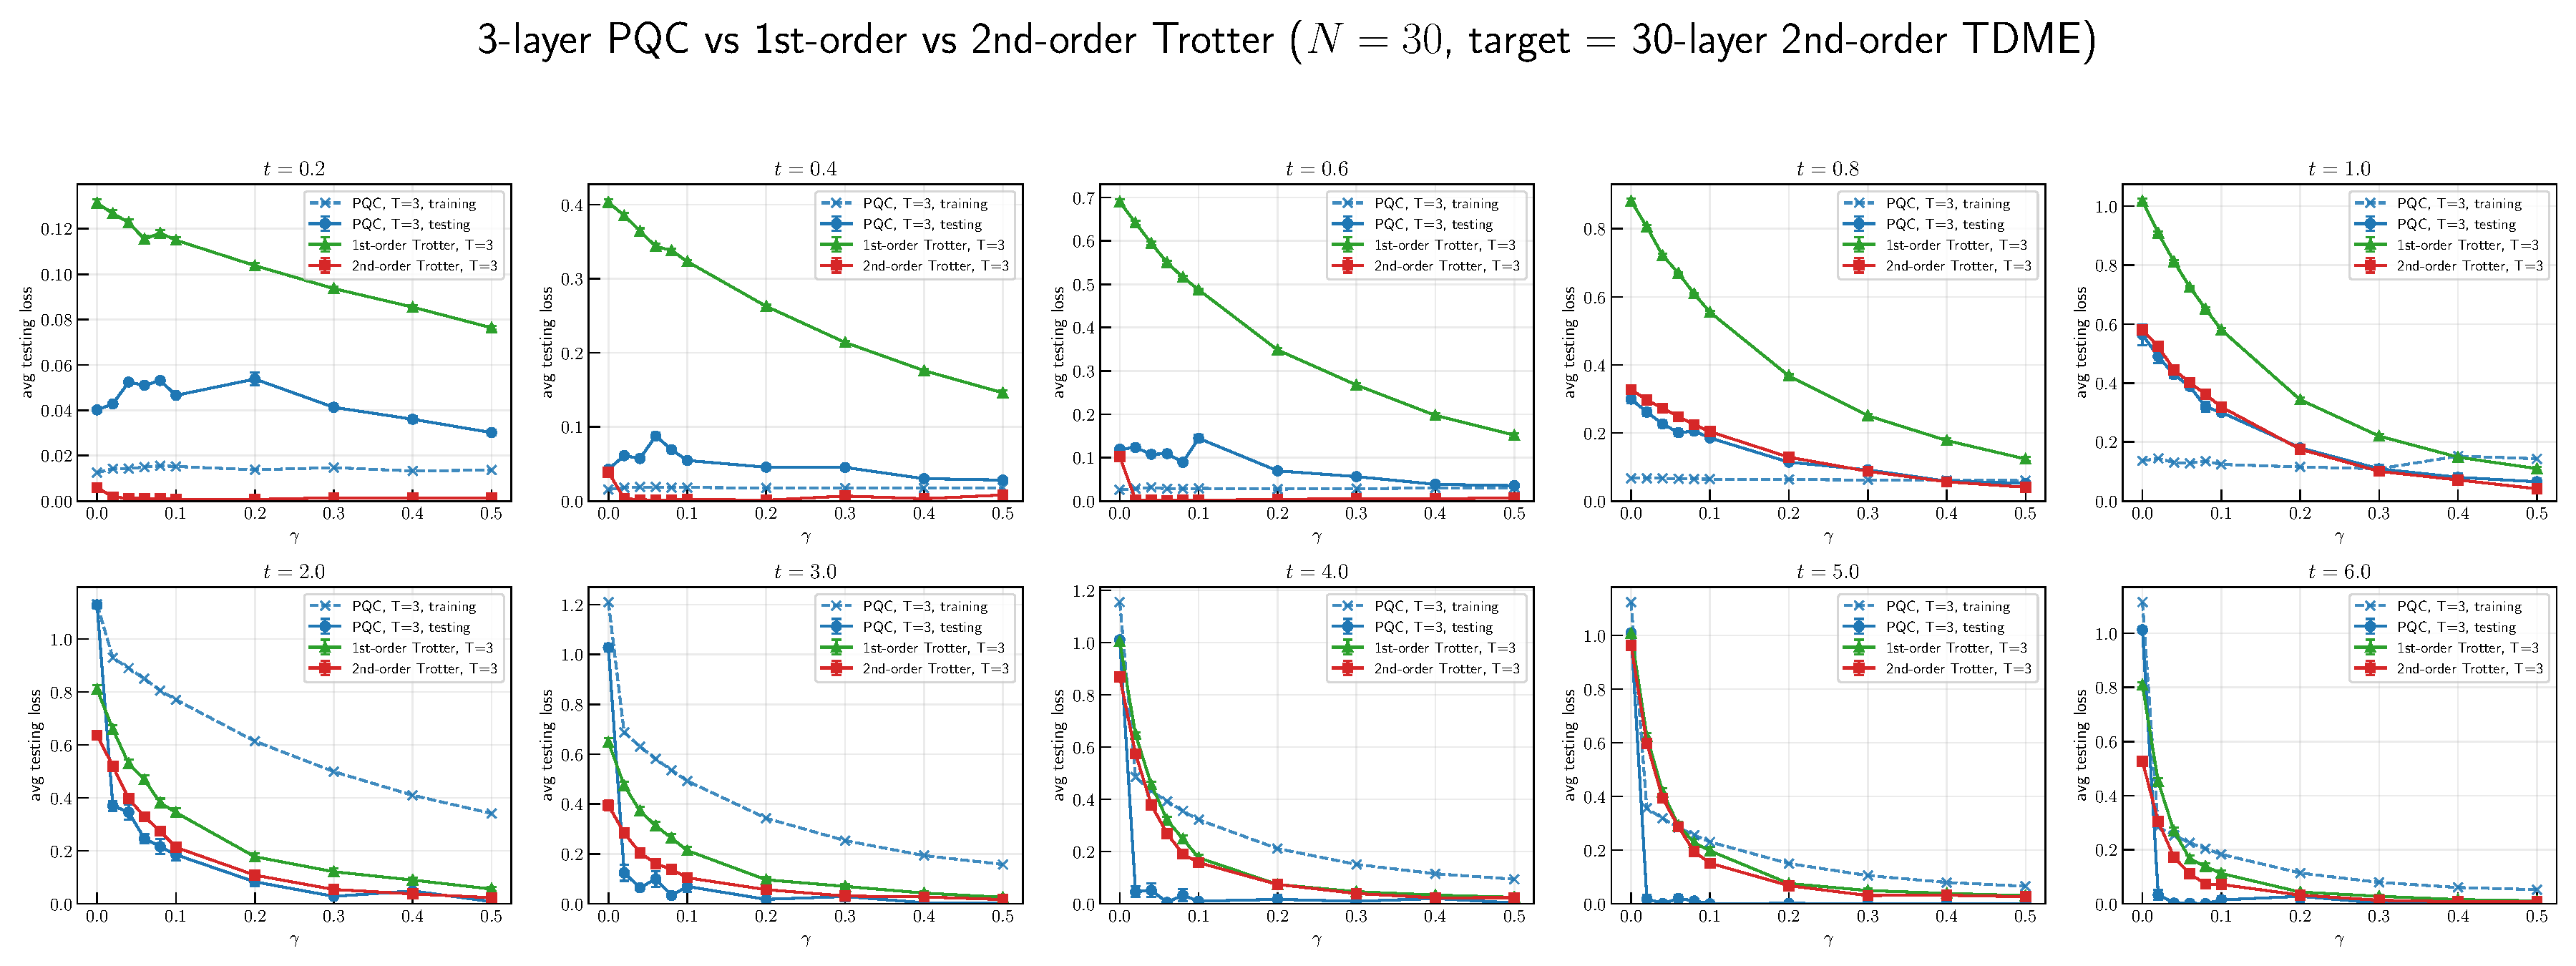
\includegraphics[width=\textwidth]{pqc_vs_trotter.pdf}
    \caption{\raggedright Testing loss versus dissipative strength $\gamma$ at $N=30$, model depth $T=3$, target depth $L=30$ (second-order Trotter), one panel per evolution time $t\in\{0.2,\ldots,6.0\}$. Each curve aggregates 300 random Pauli test inputs (PQC evaluation is on the order of 30--200 inputs depending on the shard); shaded error bars are $\pm$ standard error of the mean. Solid blue: PQC testing loss $\text{Loss}_{model}^{\text{test}}$; dashed blue: PQC \emph{training} loss (best epoch on the $3N$ weight-$1$ inputs); green triangles: $3$-layer first-order Trotter $\text{Loss}_{Trott,3}^{(1),\text{test}}$; red squares: $3$-layer second-order Trotter $\text{Loss}_{Trott,3}^{(2),\text{test}}$.}
    \label{fig:pqc_vs_trotter_N30}
\end{figure*}

Figure~\ref{fig:pqc_vs_trotter_N30} summarizes the comparison across the full $(t,\gamma)$ grid. Three regimes are visible.
\begin{enumerate}
    \item[\textbf{(i)}] \emph{Short evolution time, $t\lesssim 0.6$.} The second-order Trotter benchmark $\E_{Trott,3}^{(2)}$ achieves a testing loss below the trained $T=3$ PQC. This is the regime where the Trotter step size $\Delta t = t/T \approx 0.1$--$0.2$ is small enough that the symmetric Strang splitting -- whose per-step error scales as $\mathcal{O}(\Delta t^3)$ -- is essentially exact relative to the same target. The first-order Trotter benchmark $\E_{Trott,3}^{(1)}$ lies far above both lines: its per-step error is only $\mathcal{O}(\Delta t^2)$ and dominates here.
    \item[\textbf{(ii)}] \emph{Intermediate evolution time, $0.8\lesssim t\lesssim 2.0$.} The PQC and the second-order Trotter are close at every $\gamma$: both methods are limited by the same kind of finite-step error. The first-order Trotter trails both by a roughly constant factor of $2$--$3$, consistent with the asymptotic ratio $\sim T/t$ between first- and second-order Trotter errors at fixed depth.
    \item[\textbf{(iii)}] \emph{Long evolution time, $t\gtrsim 3$.} Naive comparison of the testing losses suggests the PQC \emph{outperforms} the second-order Trotter benchmark by factors of $2$--$60\times$. This gap is partially due to the long-evolution time causes the state to be more mixed, and the PQC structure can handle near maximally mixed states better than Trotterization.
\end{enumerate}

A way to detect the long-$t$ artifact is to compare the PQC's testing loss against its \emph{best} training loss across all epochs (the dashed blue curve in Fig.~\ref{fig:pqc_vs_trotter_N30}), recall that the training is done with the set of weight-1 Pauli strings. For $t\lesssim 1$ the testing loss is consistently \emph{higher} than the best training loss, as expected for a model that has fit the training set and now generalizes imperfectly to a broader test distribution, and also, for small $\gamma$, the resulting state is not that mixed. For $t\gtrsim 3$ the order \emph{reverses}: the PQC plateaus at a training loss that is one to three orders of magnitude \emph{larger} than its testing loss. For example, at $(t,\gamma)=(5,0.02)$ the training loss saturates near $0.36$ while the testing loss is only $0.018$. 

%This is because after a long evolution, the channel $\E_{Trott,30}^{(2)}\}$ is getting closer to a total depolarizing channel. Thus, a general weight Pauli string will have the Frobenius norm exponentially suppressed by the target channel.

The mechanism is the following. At long evolution time and non-zero $\gamma$, the target channel $\E_{Trott,30}^{(2)}$ heavily decoheres any random Pauli input that contains with $w$-weight: each such site contributes an exponential suppression $e^{-\gamma t}$ to the off-diagonal Pauli amplitudes, so for $w$-weight inputs the target output norm is $\sim e^{-\gamma t\cdot w}$, which decays rapidly with weight. For random inputs of mean weight $\sim N/2$, $\E_{Trott,30}^{(2)}(M_{test,i})$ is almost a zero operator. Meanwhile, the PQC's $T=3$ noise channels stack multiplicatively to a per-site decay $(1-p_{\text{depolar}})^T$; with the noise rates clamped near saturation, this decay overshoots that of the target, so $\E_{model}(M_{test,i})$ is even smaller in norm than the target output. The Frobenius distance between these two near-zero operators is itself near zero, but this reflects a coincidence of magnitudes rather than learned dynamics. The first-order Trotter benchmark $\E_{Trott,3}^{(1)}$ does not benefit from this magnitude-matching: at $\Delta t\gtrsim 1$ it produces a state that is wrongly \emph{rotated} (not contracted), so its Frobenius distance to the target stays $\mathcal{O}(1)$.

The shape-matched first-order Trotter comparison removes the discretization-order advantage that $\E_{Trott,3}^{(2)}$ has over the PQC. As Fig.~\ref{fig:pqc_vs_trotter_N30} shows, in this comparison the PQC outperforms the Trotter benchmark across the entire $(t,\gamma)$ grid, with geometric-mean ratios $\text{Loss}_{Trott,3}^{(1),\text{test}}/\text{Loss}_{model}^{\text{test}}$ between $1.9\times$ at $t=1.0$ and $\sim 7\times$ at $t=4.0$. The advantage is most pronounced when both the trainable unitary content and the trainable noise content of the PQC are useful: short-to-intermediate evolution times where the dynamics is non-trivial, and dissipative strengths where the noise channel is informative but not yet saturating. This confirms the qualitative claim that, at matched circuit depth and per-layer shape, a trained variational ansatz reproduces the dynamics more faithfully than a single-step naive Trotterization.

\begin{figure*}[t]
    \centering
    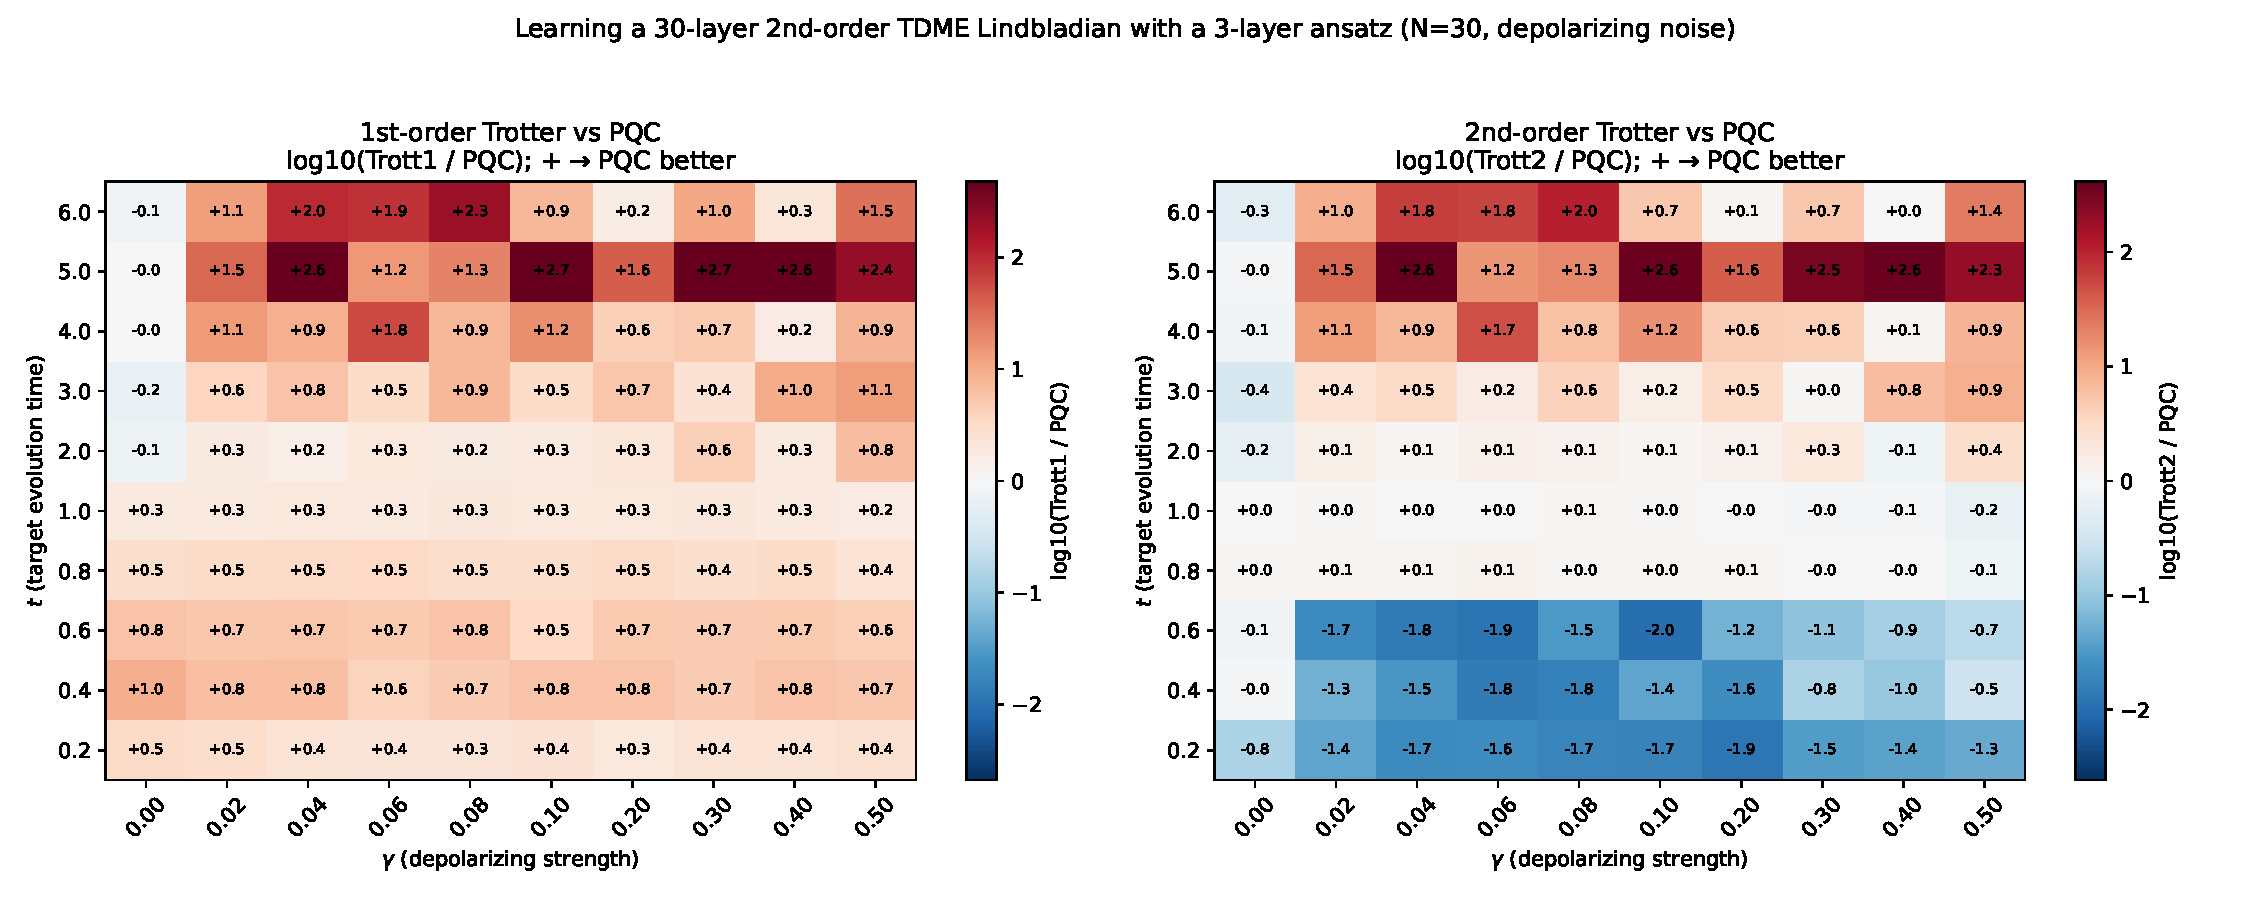
\includegraphics[width=0.8\textwidth]{heatmap_pqc_vs_trotter.pdf}
    \caption{\raggedright Heatmaps of the log-ratio $\log_{10}(\text{Trotter loss}/\text{PQC testing loss})$ over the $(t,\gamma)$ grid at $N=30$, $T=3$. Positive (red) entries denote the PQC having a lower testing loss, negative (blue) the Trotter baseline being lower. \textbf{Left:} versus the shape-matched first-order Trotter; the PQC is better essentially everywhere. \textbf{Right:} versus the second-order Trotter; the PQC is dominated at short $t$ (regime where Strang splitting is nearly exact) and tied at intermediate $t$. The deep red at long $t$ should be read against Fig.~\ref{fig:pqc_vs_trotter_N30} and the training-loss diagnostic discussed in the text.}
    \label{fig:heatmap_pqc_vs_trotter}
\end{figure*}

Figure~\ref{fig:heatmap_pqc_vs_trotter} renders the log-ratios over the full $(t,\gamma)$ grid for both Trotter benchmarks. The left panel (versus first-order Trotter) is uniformly red, confirming a depth-matched advantage for the PQC. The right panel (versus second-order Trotter) is deep blue at small $t$, white through the intermediate band, and red at long $t$ -- but the long-$t$ red region is precisely where the testing-loss vs training-loss diagnostic of Fig.~\ref{fig:pqc_vs_trotter_N30} flags the metric pathology. Taken together, the data show that the $T=3$ PQC genuinely matches the second-order Trotter performance over a wide intermediate window of evolution times and dissipative strengths at $N=30$ qubits, that it strictly improves upon a same-depth first-order Trotter, and that scaling these experiments to large system sizes does not introduce qualitative pathologies relative to the small-$N=8$ analysis of the previous subsection.


%\begin{figure}
    %\centering
    %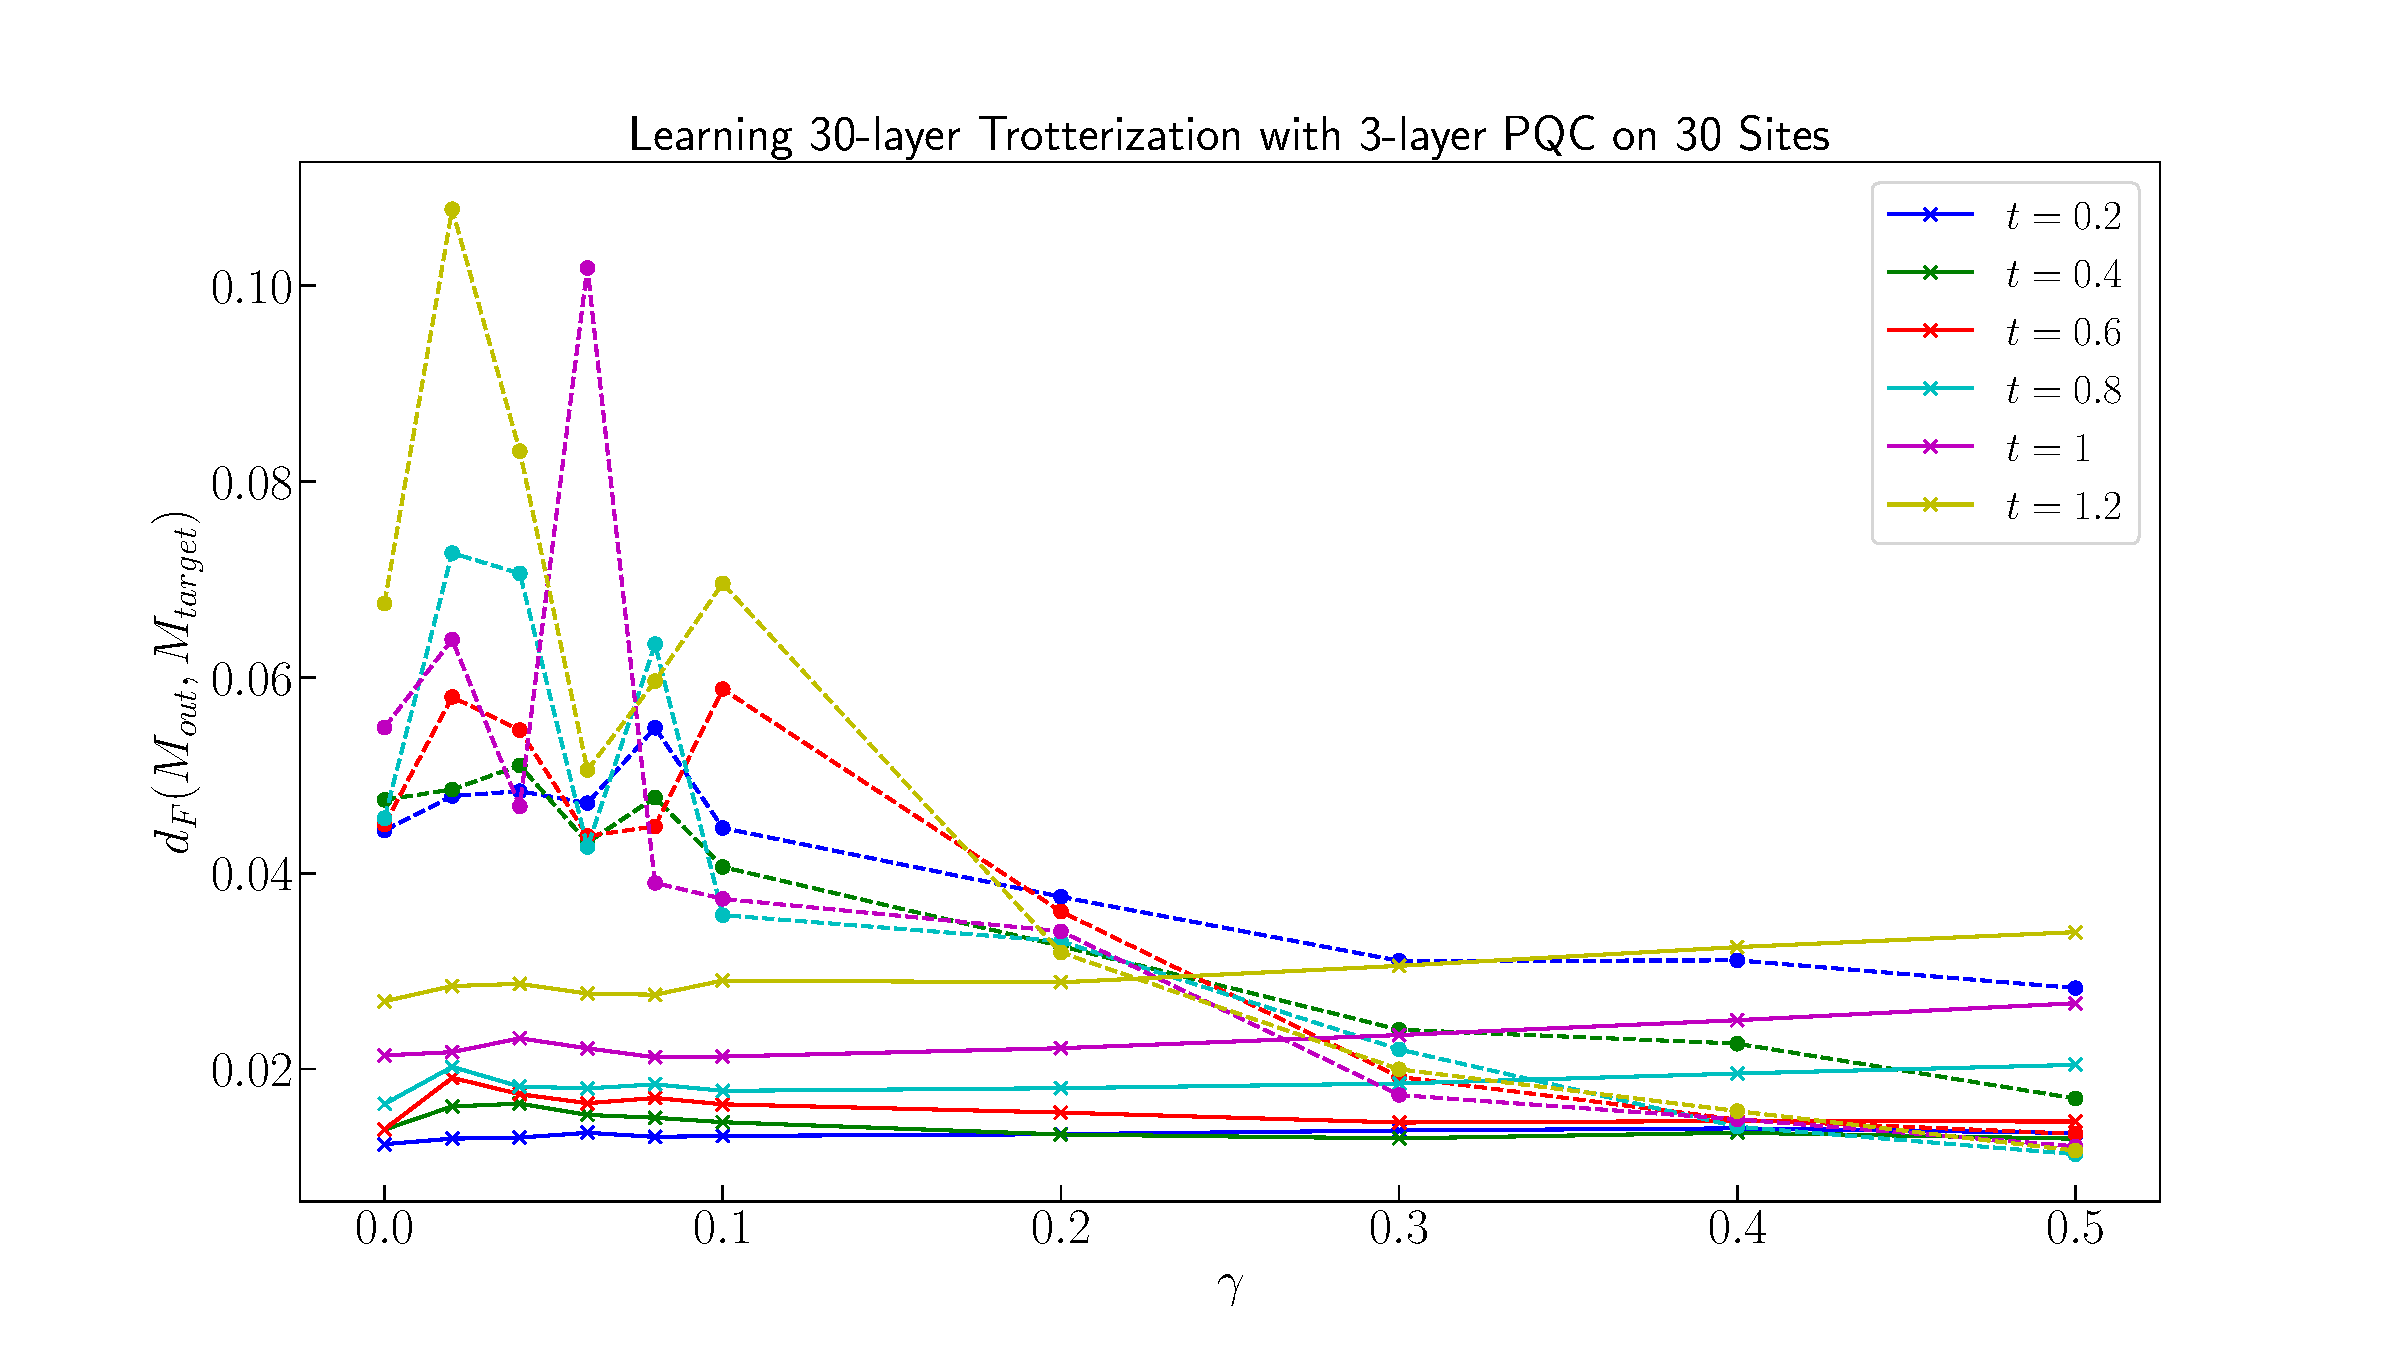
\includegraphics[width=\linewidth]{Learning_TDME_N_30_varies_gamma_time_02_12.pdf}
    %\caption{\raggedright The result of using a 3-layer PQC with $N=30$ qubit sites to learn the Lindbladian circuit with 30-layer Trotterization, and compare with using a 3-layer Trotterization for different target time $t$ and different dissipative strength $\gamma$. The solid line represents learning loss and the dotted lines represent testing loss.}
    %\label{fig:Learning_TDME_N_30_varies_gamma_time_02_12}
%\end{figure}

%Similar to the previous sections on learning a random unitary, we can learn the Lindbladian dynamics on a much larger number of qubit sites with truncation enabled, in this section, we demonstrate the results of learning a 30-site Lindbladian dynamics governed by the Master Equation ~\ref{eq:TDME_Lindbladian}, we truncate the maximum bond dimension to $64$, and we run the simulations on a computational cluster.

%The result is shown in Figure~\ref{fig:Learning_TDME_N_30_varies_gamma_time_02_12}, which demonstrates that even for a very large number of qubit sites, using our Ansatz PQC to learn a Trotterization still works pretty well.

\section{Quantum System coupled to Baths}
As a final case study of our Quantum machine learning model using PQCs, we want to see whether compression can be achieved when the quantum system is coupled to quantum baths. In the previous sections, we mainly focused on whether we can compress a given deeper quantum circuit with a shallower PQC, where the target circuit can be either a deeper PQC or the Trotterization of some Lindblad dynamics. In other words, the previous numerical parts of this paper focus on compressing the quantum circuit in depth.

In this section, we ask a different question, which is whether a quantum circuit can be compressed in width. Specifically, we are interested in a small quantum system that is coupled to an external quantum bath, and we want to understand whether it is theoretically possible to learn this system with the ansatz PQC we have introduced before.

\subsection{Setup for Learning an Open-system coupled to a bath}
\label{sec:setup_for_learning_bath}

We test the PQC ansatz on the task of learning an effective open-system channel on $N=10$ system qubits obtained by tracing out $N=10$ bath qubits from a $2N$-qubit unitary evolution. Since we are using the one-dimensional MPS system, the data and bath qubits are arranged in alternating order. Denote $d$ as the data qubits and $b$ as the bath qubits, the one-dimensional MPS during evolution is structured as $\cdots d-b-d-b\cdots$.


The target circuit $\E_{target}$ is composed of $L_{target}$ layers, each layer consisting of three sub-layers: 

\begin{enumerate}
    \item An odd brick of Haar-random two-qubit gates $\{U^{(\ell)}_{\mathrm{o},k}\}_k$ acting on adjacent pairs of data qubits.
    \item An even brick of Haar-random two-qubit gates $\{U^{(\ell)}_{\mathrm{e},k}\}_k$ on the complementary data pairs.
    \item A layer of weak data-bath interaction gates $U_{\mathrm{db}}(g) = \exp(-i\, g\, H_{\mathrm{db}})$ applied independently between every system qubit and its dedicated bath qubit
\end{enumerate} 

Where the interaction Hamiltonian is the hopping operator $H_{\mathrm{db}} = -g\,(X_d X_b + Y_d Y_b)$ with $g$ is the coupling strength. For each system--bath coupling strength $g$ and circuit depth $L$ we construct a target channel $\mathcal{E}_{g,L}$ from a depth-$L$ brick-wall unitary acting on the joint system-bath Hilbert space. 

The target channel $\mathcal{E}_{g,L}(\rho) = \operatorname{Tr}_{b}\bigl[U_{g,L},(\rho \otimes \mathbf{1}b/2^N)U_{g,L}^{\dagger}\bigr]$ assumes a maximally mixed bath; we evaluate it numerically in the Pauli-transfer-matrix representation by propagating Pauli operators through the joint circuit, with each bath site carrying the identity component $\ket{I}$ and the partial trace implemented as projection of each bath leg onto $\ket{I}$.

The model circuit $\E_{model}$ is a PQC acting only on the $N$ system qubits, which is half the size of $\E_{target}$. The structure of the model PQC $\E_{model}$ is the same as the ansatz PQC we used in previous sections, about learning random unitaries and learning a Lindblad dynamics. We match the model depth to the target, $T = L$, so the testing loss between $\E_{target}$ and $\E_{model}$ reflects the architectural mismatch between this strictly Markovian depolarising ansatz PQC and a possibly non-Markovian bath-traced channel.

During the simultaion, we sweep across $g \in \{0,\, 0.05,\, 0.10,\, \dots,\, 0.50\}$ to interpolate between a closed unitary target ($g=0$) and a strongly dissipative channel ($g=0.5$), and vary $L \in \{2,3,4,5\}$ to probe how the depth of the system--bath interaction affects learnability. For each data point, we have run over at least 40 samples and calculated the average with the error bar representing 1 standard deviation.

Similar to before, the training dataset consists of the full set of $3N$ weight-1 Pauli inputs, with the loss defined as the squared Frobenius distance between the model's Pauli-basis output and the target's bath-traced target, evaluated as a tensor-network contraction. 

%After training, we report (a) the train loss on the $3N$ weight-1 inputs and (b) an average test loss over $100$ random Pauli strings drawn uniformly from $\{I,X,Y,Z\}^{\otimes N}$ and evaluated on the same teacher; each $(T_L,g)$ point is repeated over five independent teacher seeds and we quote the mean with $\pm 1\sigma$ error bars.

\subsection{Results}
\begin{figure*}
    \centering
    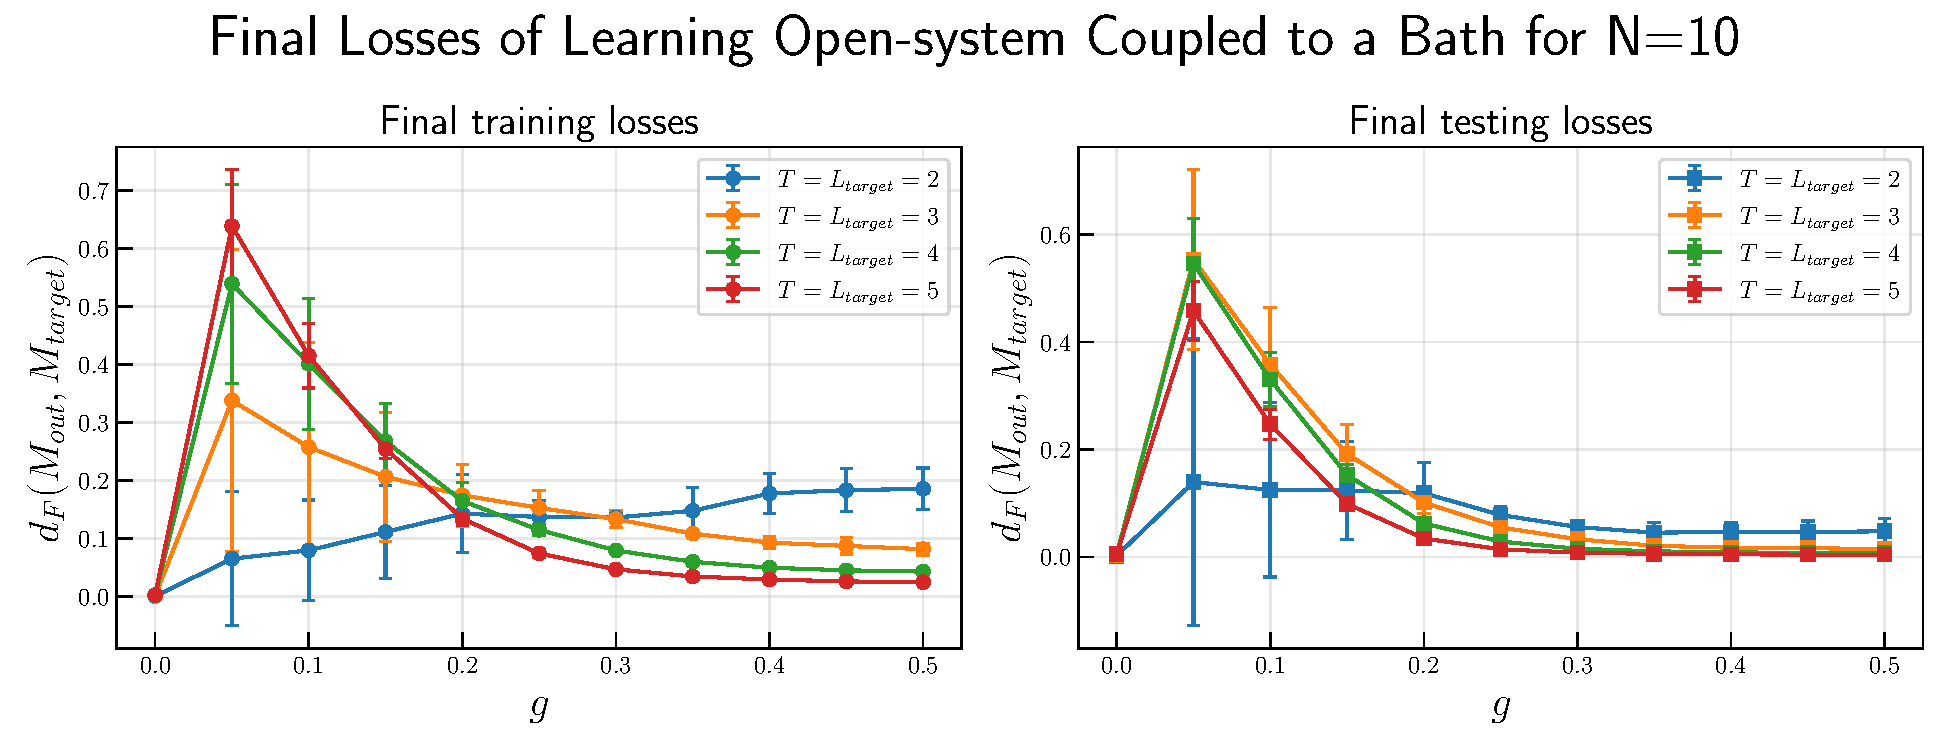
\includegraphics[width=0.8\textwidth]{bath_sweep_N10_final_vs_g_all_TL.pdf}
    \caption{\raggedright The final losses of learning an open-system that is coupled to a bath with $N=10$, with the construction described in section~\ref{sec:setup_for_learning_bath}. We see very clear that for $T = L_{target}$ and for $g=0$, the learning process can be done perfectly. While for $g>0$, the hardest case for learning is always at small $g$, where the non-unitary effect dominant. And when the bath coupling $g$ becomes larger, the learning and testing loss drops again.}
    \label{fig:bath_sweep_N10_final_vs_g_all_TL}
\end{figure*}

As shown in Figure~\ref{fig:bath_sweep_N10_final_vs_g_all_TL}, the results is similar 

\section{Conclusion}

In this work, we have addressed the critical challenge of learning and compressing deep quantum circuits and continuous time evolutions within the noisy intermediate-scale quantum (NISQ) regime. Recognizing the limitations of standard state-basis learning---which often relies on costly ancilla qubits to mimic non-unitary dynamics---we rigorously formulated our learning framework in the operator basis. By utilizing the Pauli Transfer Matrix (PTM) and optimizing the Frobenius distance, we established a robust, resource-efficient method for Parameterized Quantum Circuits (PQCs) to learn and emulate general completely positive trace-preserving (CPTP) maps.

Theoretically, we derived strict upper bounds on the generalization error for quantum machine learning models representing such CPTP maps, proving that the required number of training samples scales favorably with the model complexity. A primary theoretical insight of our work is the intrinsic connection between Local Operator Entanglement (LOE) and the learnability of Matrix Product States (MPS). We mathematically demonstrated that non-unitary operations, such as depolarizing and dephasing noise, naturally suppress the growth of operator entanglement. This suppression bounds the required bond dimension in tensor networks, offering a fundamental physical explanation for why noisy quantum channels admit highly compressed, shallow-depth PQC representations compared to their noiseless unitary counterparts.

Numerically, our extensive simulations validate these theoretical predictions. By introducing a novel PQC architecture that interleaves two-site trainable unitaries with parameter-dependent single-site noise layers, we successfully compressed both deep Haar-random channels and intricate open-system dynamics. For generic noisy circuits, we showed that moderately shallow PQCs accurately substitute much deeper target circuits. Furthermore, we scaled our tensor-network simulations up to 30 qubits by judiciously employing bond-dimension truncations, noting that the truncation errors were inherently mitigated by the physical presence of noise. 

Beyond random unitaries, we demonstrated the practical impact of our framework by applying it to the Trotterized evolution of one-dimensional Lindbladian dynamics governed by a time-dependent master equation. Our results confirm that a compact 3-layer PQC can faithfully reproduce the dynamics of a heavily Trotterized 30-layer sequence, significantly outperforming standard shallow Trotterization over extended evolution times.

Looking forward, this methodology points towards several exciting research directions. Our observation that quantum noise surprisingly facilitates circuit compression implies that hardware-tailored variational compilation could act as an inherent noise-mitigation and model-parsimony strategy. Future studies could extend our operator-basis learning approach to higher-dimensional topologies, such as 2D and 3D lattices, or incorporate more complex asymmetric noise channels like amplitude damping and correlated crosstalk. Ultimately, empirical demonstrations of our proposed compression protocols on state-of-the-art quantum processors will solidify their utility for quantum-assisted compiling, benchmarking, and the efficient simulation of complex open quantum systems.

\bibliography{Quantum_Channel_Learning}

\end{document}
